%\documentclass[11pt][fleqn]{report}
\documentclass[fleqn,10pt]{book}

\usepackage{bm,amsmath}
\usepackage{makeidx}
\usepackage{color}
\usepackage{natbib}
\usepackage{mfpic}
\usepackage{pxfonts}
\usepackage{lastpage}
\usepackage{graphicx}
\usepackage{verbatim} 
\usepackage{authblk}
\usepackage{tikz}
\usepackage[framemethod=tikz]{mdframed}

\usepackage{titlesec}
\titleformat*{\section}{\LARGE\bfseries}
\titleformat*{\subsection}{\Large\bfseries}
\titleformat*{\subsubsection}{\large\bfseries}
\titleformat*{\paragraph}{\large\bfseries}
\titleformat*{\subparagraph}{\large\bfseries}
\renewcommand{\familydefault}{\sfdefault}

\newcommand{\bftau}{\mbox{\boldmath $\tau$}}


\usepackage{minitoc} 
\renewcommand{\mtcfont}{\small\sffamily} 
\renewcommand{\mtcSfont}{\small\sffamily} 
\usepackage[Lenny]{fncychap}

\evensidemargin -.3in
\oddsidemargin  0.0in

\topmargin -0.50in
\textheight 9.0in
\renewcommand{\baselinestretch}{1.0}
\textwidth 6.5in

\usepackage{fancyhdr}
\pagestyle{fancy}
\fancyhf{}
\lhead{\leftmark}
\rhead{Section \thesection}
\lfoot{{\sc Column tests of CVMix/KPP}}
\cfoot{\today}
\rfoot{Page \thepage}
\renewcommand{\footrulewidth}{1pt}
\usepackage{kpfonts}
\fancyhead[LE,LO]{\textsc{\textbf{\nouppercase{\leftmark}}}}

\usepackage{titlesec,titletoc} 
\titleclass{\part}{top}
\titleformat{\part}
{\centering\normalfont\Huge\bfseries}{}{0pt}{}

\usepackage{hyperref}  % must be used last in the list of packages 
\hypersetup{colorlinks=true,linkcolor=blue,citecolor=blue,filecolor=blue,urlcolor=blue} 


\setcounter{tocdepth}{1}
\setcounter{minitocdepth}{3}
\setcounter{secnumdepth}{3}

\makeindex 
\citeindextrue

\title{\sc Column tests of CVMix/KPP}

\date{\today}

% \author[$\star$]{Stephen M. Grif\/f\/ies \thanks{Stephen.Griffies@noaa.gov}}
% \affil[$\star$]{NOAA/Geophysical Fluid Dynamics Laboratory, Princeton USA}

% \author[$\dagger$]{Michael Levy \thanks{MLevy@ucar.edu}}
% \affil[$\dagger$]{National Center for Atmospheric Research, Boulder USA}

% \author[$\star$]{Alistair J. Adcroft \thanks{Alistair.Adcroft@noaa.gov}}
% \author[$\dagger$]{Gokhan Danabasoglu \thanks{Gokhan@ucar.edu}}
% \author[$\star$]{Robert W. Hallberg \thanks{Robert.Hallberg@noaa.gov}}

% \author[$\triangle$]{Doug Jacobsen \thanks{Jacobsen.douglas@gmail.com}}
% \affil[$\triangle$]{Los Alamos National Laboratory, Los Alamos USA}

% \author[$\dagger$]{William Large \thanks{Wily@ucar.edu}}
% \author[$\triangle$]{Todd Ringler \thanks{Ringler@lanl.gov}}


\author[$\star$]{The CVMix Team}

\begin{document}

\pagenumbering{roman}
\maketitle 
\thispagestyle{empty}


\begin{center}
{\scshape \Large Column tests of CVMix/KPP} 
\end{center}

This document details tests with the KPP \citep{LargeKPP} boundary
layer parameterization in CVMix.  The ocean primitive equations are
time stepped in the ocean models MOM6, MPAS-ocean, and POP, with each
model having implemented CVMix/KPP.  The models are configured in
two-dimensional (x,y) periodic domains so that there are no lateral
gradients.  Furthermore, each uses the same grid spacing and time
step.  However, time stepping schemes differ, thus precluding bitwise
answer agreements.  Indeed, answer differences can be far more than
roundoff, illustrating the sensitivity of the KPP scheme to time
stepping details.  Physical and numerical aspects of CVMix/KPP are
provided in {\sc Theory and Numerics of the Community Ocean Vertical
  Mixing (CVMix) Project}.  Salient points from that document are
assumed here.

As there are no lateral gradients, evolution of velocity and tracer
are one-dimensional in the vertical.  We generally initialize velocity
at zero, so that it evolves only when there is a nonzero surface
stress.  If tracers have a uniform initial profile, their evolution is
initiated by buoyancy forcing via surface heating.  Once a nontrivial
vertical profile is established, either through boundary fluxes or the
initial profile, then evolution is impacted by the local portion of
KPP realized as downgradient diffusion.  Additionally, when surface
buoyancy forcing is negative, tracers are impacted by the non-local
portion of KPP.  The non-local operator redistributes the negative
surface buoyancy forcing throughout the boundary layer.


\dominitoc
\tableofcontents
\listoffigures

\pagenumbering{arabic}

\chapter{Common elements to the tests}
\label{chapter:common_elements}

In this chapter, we document common elements for the test cases.

\minitoc


\section{Heat equation and notation}

In these test cases, buoyancy is forced via a surface heat flux, which
is either zero, positive, or negative.  To help develop notation,
consider the finite-volume one-dimensional heat budget for a surface
ocean grid cell
\begin{equation}
  \mbox{C}_{\mbox{\footnotesize p}} \left(   \frac{\partial  \, (\Theta \, \rho \, \mathrm{d}z )}{\partial t}  \right) =  
  Q + F_{\mbox{\footnotesize diffusive}} + F_{\mbox{\footnotesize non-local}}.
\label{eq:surface-heat-equation}
\end{equation}
All lateral transport terms are dropped given that these tests
exercise just the vertical transport.  The following terms appear in
this equation.
\begin{itemize}

\item Conservative temperature, $\Theta$, is approximated in these
  tests with potential temperature, $\theta$.  Indeed, since the
  equation of state is linear and without pressure dependence (Section
  \ref{subsection:equation-of-state}), there is no distinction between
  Conservative, potential, or {\it in situ} temperatures.

\item The mass per unit area of a grid cell is written as $\rho \,
  \mathrm{d}z$.  For a Boussinesq model, $\rho$ in the tracer budget
  is set to the constant reference density $\rho_{0}$.  Each ocean
  model makes the Boussinesq approximation for the tests documented
  here.  The grid cell thickness, $\mathrm{d}z$, is generally a
  function of time, as in MPAS-ocean and MOM6, in which case we keep
  it inside the time derivative to ensure a flux-form budget.  If the
  cell thickness is static, as in POP, then it can be removed from the
  time derivative.\footnote{Note that for hydrostatic non-Boussinesq
    fluids, $\rho \, \mathrm{d}z = -g^{-1} \, \mathrm{d}p$, measures
    the mass per unit horizontal area for the grid cell, with
    $\mathrm{d}p$ the pressure increment for the cell.}

\item The surface boundary heat flux, $Q$, crosses the top of the
  surface cell.  The different test cases use various heat heat flux
  specifications.

\item The diffusive heat flux, $F_{\mbox{\footnotesize diffusive}}$,
  arises from the local downgradient diffusive portion of the KPP
  scheme.  This flux passes through the bottom face of the top grid
  cell.

\item The non-local KPP term, $F_{\mbox{\footnotesize non-local}}$, is
  non-zero only when the surface buoyancy flux is negative.  The
  non-local term acts to redistribute the negative surface buoyancy
  flux throughout the boundary layer.  The non-local term vanishes at
  the base of the boundary layer.

\end{itemize}




\section{Configuration details}
\label{section:configuration-details-winds_alone}

We provide configuration details in this section.  


\subsection{Vertical grids and time steps}

As detailed in Table \ref{table:kpp-model-configuration}, we consider
various vertical grid configurations for each ocean model (MOM6,
MPAS-ocean, and POP). These tests serve as a platform to examine
differences arising from coarsening the vertical resolution.

%%%%%%%%%%%%%%%%%%%% model configurations%%%%%%%%%%%%%%%%%%%%%%%%
\begin{table}[h!t]
\centering{
\begin{tabular}{|c|c|c|c|}
\hline 
{\sc model}                        & {\sc vertical grid spacing/grid points}    & {\sc bottom depth}   &    {\sc time step (secs)} \\
\hline 0.4m              & $\Delta z = 0.4~\mbox{m}$                     & $400~\mbox{m}$      & $\Delta t = 20 * 60$     \\                               
\hline 1m                 & $\Delta z = 1.0~\mbox{m}$                      & $400~\mbox{m}$      & $\Delta t = 20 * 60$     \\                               
\hline 10m               & $\Delta z = 10.0~\mbox{m}$                    & $400~\mbox{m}$      & $\Delta t = 20 * 60$      \\                               
\hline MOM6-CM4             &  75                                                   & $6500~\mbox{m}$    & $\Delta t = 20 * 60$      \\
%\hline MPAS-ACME             &  ??                                                             & ??                            & $\Delta t = ??$             \\
%\hline POP-CESM                & ??                                                            & ??                              & $\Delta t = ??$             \\
\hline
\end{tabular}
}
\caption{Model vertical grid spacing, bottom depth,  and time steps
  for the CVMix column tests.  Note that each test 
  with MOM6 was run on a workstation, which constrains the size of the
  finest grid spacing.   The MOM6-CM4 vertical spacing corresponds to
  the spacing used in the CM4 global climate model being developed 
  at GFDL.}
\label{table:kpp-model-configuration}
\end{table}
%%%%%%%%%%%%%%%%%%%%%%%%%%%%%%%%%%%%%%%%%%%%%%%%%%%%%%%%%%%%%%%%%%%%%%%%


\subsection{Basic constants and linear equation of state}
\label{subsection:equation-of-state}

The basic constants used for the tests are given by the gravitational
acceleration, the Coriolis parameter, and the heat capacity, each of
which are global constants.
\begin{subequations}
\begin{align}
 g &= 9.80616~\mbox{m}~\mbox{s}^{-2}
 \\
 f &= 1.0 \times 10^{-4}~\mbox{s}^{-1}
 \\
\mbox{C}_{\mbox{\footnotesize p}} &= 3992.1~\mbox{J}~\mbox{kg}^{-1}~\mbox{K}^{-1}. 
\end{align}
\end{subequations}
We offer the following comments.
\begin{itemize}
\item A non-zero Coriolis parameter allows for inertial oscillations
  in the vertical column test cases, with periods 
\begin{equation}
   T_{\mbox{\footnotesize inertial}} = \frac{2 \, \pi}{f} = 0.73~\mbox{day}.
\label{eq:inertial-period}
\end{equation}
Consequently, inertial oscillations are a prominent feature in the
velocity field realized in these tests.

\item The heat capacity is needed to convert from a heat flux to a
  temperature flux.  The chosen value accords with the first five
  significant digits of the \cite{TEOS2010} value.

\end{itemize}
The equation of state for density is linear, and a function only of
temperature and salinity 
\begin{equation}
\rho = \rho_0 - \alpha \, (\Theta - \Theta_0) + \beta \, (S-S_0).
\label{eq:linear-eos}
\end{equation}
The equation of state constants are given by 
\begin{subequations}
\begin{align}
 \rho_0 &= 1000.00~\mbox{kg}~\mbox{m}^{-3}
\label{eq:linear-eos-paramA}
 \\
\alpha &= 2.55 \times 10^{-1}~\mbox{kg}~\mbox{m}^{-3}~^{\circ}C^{-1}
\\
\beta &= 7.64\times10^{-1}~\mbox{kg}~\mbox{m}^{-3}~\mbox{ppt}^{-1}
 \\
T_0  &=  19^{\circ}C 
\\
S_0 &=  35~\mbox{ppt}.
\label{eq:linear-eos-paramB}
\end{align}
\end{subequations}
  Given that the equation of state is linear, there is no distinction
  between Conservative temperature, potential temperature, or {\it in
    situ} temperature.  



\subsection{Initial Conditions}

We start the velocity field with zero value throughout the column
\begin{equation}
 {\bf v} = 0.
\end{equation}
Surface stress imparts a vertical shear in the horizontal velocity.  A
vertical viscosity will then transfer momentum vertically.  Salinity
is initialized to the constant value
\begin{equation}
 S = S_{0}.
\end{equation}
There are no salt fluxes through the boundaries, so that salinity
remains constant throughout these tests.  Checking that it indeed
remains constant is a useful means to test that the model code is
properly conserving the salt content, both locally and globally
\citep{GriffiesPacSchmidtBalaji2001}.  The temperature is initialized
either as a uniform constant of $ \Theta_s = 15.0^{\circ}\mbox{C}$
(winds plus heating test in Chapter \ref{chapter:winds_and_heating}),
or with a linear vertical stratification
\begin{subequations}
\begin{align}
 \Theta(z) &= \Theta_s + \Gamma \, z  
\label{eq:linear-stratification}
\\
 \Theta_s&= 15.0^{\circ}\mbox{C} 
\label{eq:thetas}
\\
 \Gamma  &= 0.01^{\circ}\mbox{C}~\mbox{m}^{-1}. 
\end{align}
\end{subequations}
Even without a surface buoyancy flux, temperature will evolve in the
presence of a nonzero vertical diffusivity.  With the linear equation
of state (\ref{eq:linear-eos}) and parameters
(\ref{eq:linear-eos-paramA})-(\ref{eq:linear-eos-paramB}), the initial
vertical temperature stratification leads to an initial buoyancy
frequency
\begin{subequations}
\begin{align}
 N &= \left(-\frac{g}{\rho_{0}} \frac{\partial \rho}{\partial z} \right)^{1/2}
 \\
   &= \left( \frac{g \, \alpha \, \Gamma}{\rho_{0}} \right)^{1/2}
\\
  &= 4.94 \, \times \, 10^{-3}~\mbox{s}^{-1}
 \\
 &= 49.4 \, f.
\end{align}
\end{subequations}
We are movitated to initialize the heating case with uniform
temperature in order to record the development of nontrivial
stratification under heating. 


\subsection{Boundary conditions}

We assume the following boundary conditions.
\begin{itemize}

\item We assume a constant zonal stress and zero meridional stress at
  the ocean surface
\begin{subequations}
\begin{align}
 \tau^{x} &=  0.1~\mbox{N}~\mbox{m}^{-2}
 \\
 \tau^{y} &=  0.
\end{align} 
\end{subequations}

\item Zero buoyancy flux passes through the ocean bottom.

\item Constant surface boundary heat flux, either zero, positive, or
  negative.

\item We considered a test case with a restoring surface boundary
  condition.  The results were found to be quite similar to the
  constant positive heat case.  Hence, the restoring test case was
  dropped in order to streamline testing. However, it may prove of use
  in future tests, which motivates providing the following details.

  The restoring heat flux given by
\begin{equation}
 Q =  \rho_o \, \mbox{C}_{\mbox{\footnotesize p}} \, w_{\mbox{\footnotesize piston}} \, (\Theta_{\mbox{\footnotesize restore}}  - \Theta),
\label{eq:heat-flux-restoring}
\end{equation}
 where the restoring temperature is 
\begin{equation}
\Theta_{\mbox{\footnotesize restore}}  = \Theta_s + 10^{\circ}C,
\label{eq:restoring-temp}
\end{equation}
 and the piston velocity is 
\begin{equation}
  w_{\mbox{\footnotesize piston}} = 0.5~\mbox{m}~\mbox{day}^{-1}. 
\end{equation}
With these parameters, the restoring boundary condition produces a
heat flux, per degree temperature deviation
$\Theta_{\mbox{\footnotesize restore}} - \Theta$, given by
\begin{subequations}
\begin{align}
 \frac{Q}{(\Theta_{\mbox{\footnotesize restore}} - \Theta )} &= \rho_o \, \mbox{C}_{\mbox{\footnotesize p}} \, w_{\mbox{\footnotesize piston}}
 \\
 &= 23.68~\mbox{W}~\mbox{m}^{-2}~\mbox{K}^{-1}.  
\end{align}
\end{subequations}
That is, with $\Theta_{\mbox{\footnotesize restore}} - \Theta =
1~\mbox{K}$, we have $Q = 23.68~\mbox{W}~\mbox{m}^{-2}$.  This heat
flux is always non-negative, so it causes the ocean temperature to
initially increase quite rapidly as driven by
$\Theta_{\mbox{\footnotesize restore}} - \Theta_s = 10^{\circ}C$, and
with a decreasing (still non-negative) heat flux as the surface
temperature approaches $\Theta_{\mbox{\footnotesize restore}}$.  

\end{itemize}



\subsection{CVMix/KPP parameter settings}

The following KPP parameters are set for these tests. 
\begin{itemize}

\item Critical Richardson number is set to the standard value $\mbox{Ri}_{\mbox{\footnotesize c}} = 0.3$.

\item The background viscosity and diffusivity are both set to zero,
  so that the only means of diffusing tracer or velocity arises from
  the KPP diffusivity.

\item The KPP boundary layer interpolation type is set to {\tt cubic}.

\item The surface layer thickness occupies 10\% of the KPP boundary
  layer depth.  This thickness generally spans more than just the
  surface grid cell.  If one instead assumes the surface layer is just
  the surface grid cell (not recommended), then simulation results
  will differ from those presented here.

\item The non-local term is treated via the {\tt SimpleShapes} option.

\end{itemize}


\section{Diagnostics}

We aim to evaluate the simulation in various ways, both to expose the
physical processes and to allow for detailed comparison across a suite
of models implementing the CVMix/KPP scheme.  We list certain of the
diagnostics in Table \ref{table:metrics} of use for this purpose.
Ideally, all models will produce the same results.  However, we have
found that results can depend on the differences in time stepping
schemes used by the models (leap-frog with periodic Euler backward in
POP; forward-backward in MOM6; and Runga-Kutta in MPAS-O).  

\begin{table}[htdp]
\begin{center}
\begin{tabular}{|c|c|c|c|c|}
\hline
{\sc quantity}                                 & {\sc name}        & {\sc units}                              & {\sc output sampling}     & {\sc comments} \\
\hline
surface boundary-layer depth          & $OBL$              & $\mbox{m}$                            & $\Delta t$                       &  \\
\hline 
mixed layer depth                           & $MLD$              & $\mbox{m}$                            & $\Delta t$                       &  \\
\hline 
sea-surface temperature                 & $SST$               & $^{\circ}C$                                & $\Delta t$                       & $SST=\Theta(k=1)$\\
\hline 
% surface buoyancy flux                     & $B_{f}$              & $\mbox{m}^2~\mbox{s}^{-3}$   &$\Delta t$                    &  \\
% \hline 
% position of layer interfaces              & $z_I$                & $\mbox{m}$                             & $\Delta t$ &  \\
% \hline 
temperature                                    & $\Theta$         & $^{\circ}C$                                  &  $\Delta t$  &  all vertical levels \\
\hline
 zonal velocity component               & $u$                   & $\mbox{m}~\mbox{s}^{-1}$       &  $\Delta t$  &  all vertical levels \\
\hline 
%meridional velocity component       & $v$                    & $\mbox{m}~\mbox{s}^{-1}$       &  $\Delta t$  &  all vertical levels \\
%\hline
\end{tabular}
\end{center}
\caption{Table of diagnostics for the various test cases. 
  The first output should be at the initial condition, $t=0$. The final 
  output is at the end of the test, at $t=15~\mbox{days}$.  
  All vertical grid points are sampled, and all time steps are
  sampled. SST is diagnosed at the temperature in the top model grid
  cell.  The mixed layer depth is diagnosed as the depth where the
  potential density referenced to the surface differs from the surface
  potential density by $0.003~\mbox{kg}~\mbox{m}^{-3}$.  The mixed layer
  depth does not equal to the boundary layer depth, so it is useful to
  diagnose both.}
\label{table:metrics}
\end{table}




\chapter{Wind stress with zero buoyancy forcing}
\label{chapter:wind_alone}

In this chapter, we document a test case configured with a constant
zonal wind stress 
\begin{equation}
 \bftau  =  (0.1, 0)~\mbox{N}~\mbox{m}^{-2}
\end{equation}
and zero heat flux
\begin{equation}
Q=0~\mbox{W}~\mbox{m}^{-2}.
\end{equation}
The temperature is initialized with a stable linear stratification
according to equation (\ref{eq:linear-stratification}).  This test
ilustrates how mechanical forcing induces mixing into vertically
stratified water.  This test furthermore exercises only the local
downgradient diffusive portion of KPP, as the non-local KPP term
vanishes with a zero surface buoyancy flux.  Although somewhat
trivial, this test has proven useful for ensuring that implementation
details are consistent across ocean models making use of CVMix/KPP.

\minitoc


\section{Results from GFDL-MOM6}
\label{section:wind_only_mom6}

Figure \ref{fig:MOM6_SST_bldepth-wind_alone} shows the KPP boundary
layer depth and mixed layer depth realized from the MOM6
implementation of CVMix.  The boundary layer deepens in time, due to
the mechanical forcing from winds that eats away at the vertical
stratification.  Correspondingly, the SST cools as mixing entrains
cooler water from below.  Note how the mixed layer depth closely
follows the SST, whereas the boundary layer depth oscillates according
to the inertial oscillations.  Furthermore, note the plateaus
exhibited in the KPP boundary layer depth, particularly by the
$10~\mbox{m}$ simulation.  Such behaviour is discussed in Appendix D
of \cite{LargeKPP}.  The plateaus are less visible in the mixed layer
depth.

As furthermore discussed in Appendix D of \cite{LargeKPP}, there is a
dependence on vertical grid resolution in Figure
\ref{fig:MOM6_SST_bldepth-wind_alone}, with deeper boundary layer and
cooler SST found as the vertical grid coarsens.  The reason for the
cooler SST with coarser grids is that the KPP vertical diffusivity is
directly proportional to the boundary layer thickness, which is seen
in the lower panels of Figure \ref{fig:MOM6_SST_bldepth-wind_alone}.
Hence, deeper boundary layers produce more vertical mixing of warm
surface waters with cooler deeper waters, thus producing cooler SSTs
and warmer interior waters.  This mixing is further seen from the
depth profiles of temperature in Figure
\ref{fig:MOM6_temp-wind_alone}.  With coarser vertical grids and the
associated enhanced vertical mixing, there is an enhanced surface
cooling and deep warming relative to results from the fine vertical
grids.

Inertial oscillations in the zonal velocity are shown in Figure
\ref{fig:MOM6_zonal-wind_alone}.  The amplitude of the oscillations is
enhanced as the vertical resolution is refined.  The oscillations
impart an oscillation in the vertical shear, which in turn impacts on
the boundary layer depth.  This is the primary reason that the
boundary layer depth shows oscillations in Figure
\ref{fig:MOM6_SST_bldepth-wind_alone}.  

%%%%%%%%%%%%%%%%%%%% %%%%%%%%%%%%%%%%%%%%%%%%%
\begin{figure}[h!t]
%\rule{\textwidth}{0.005in}
\begin{center}
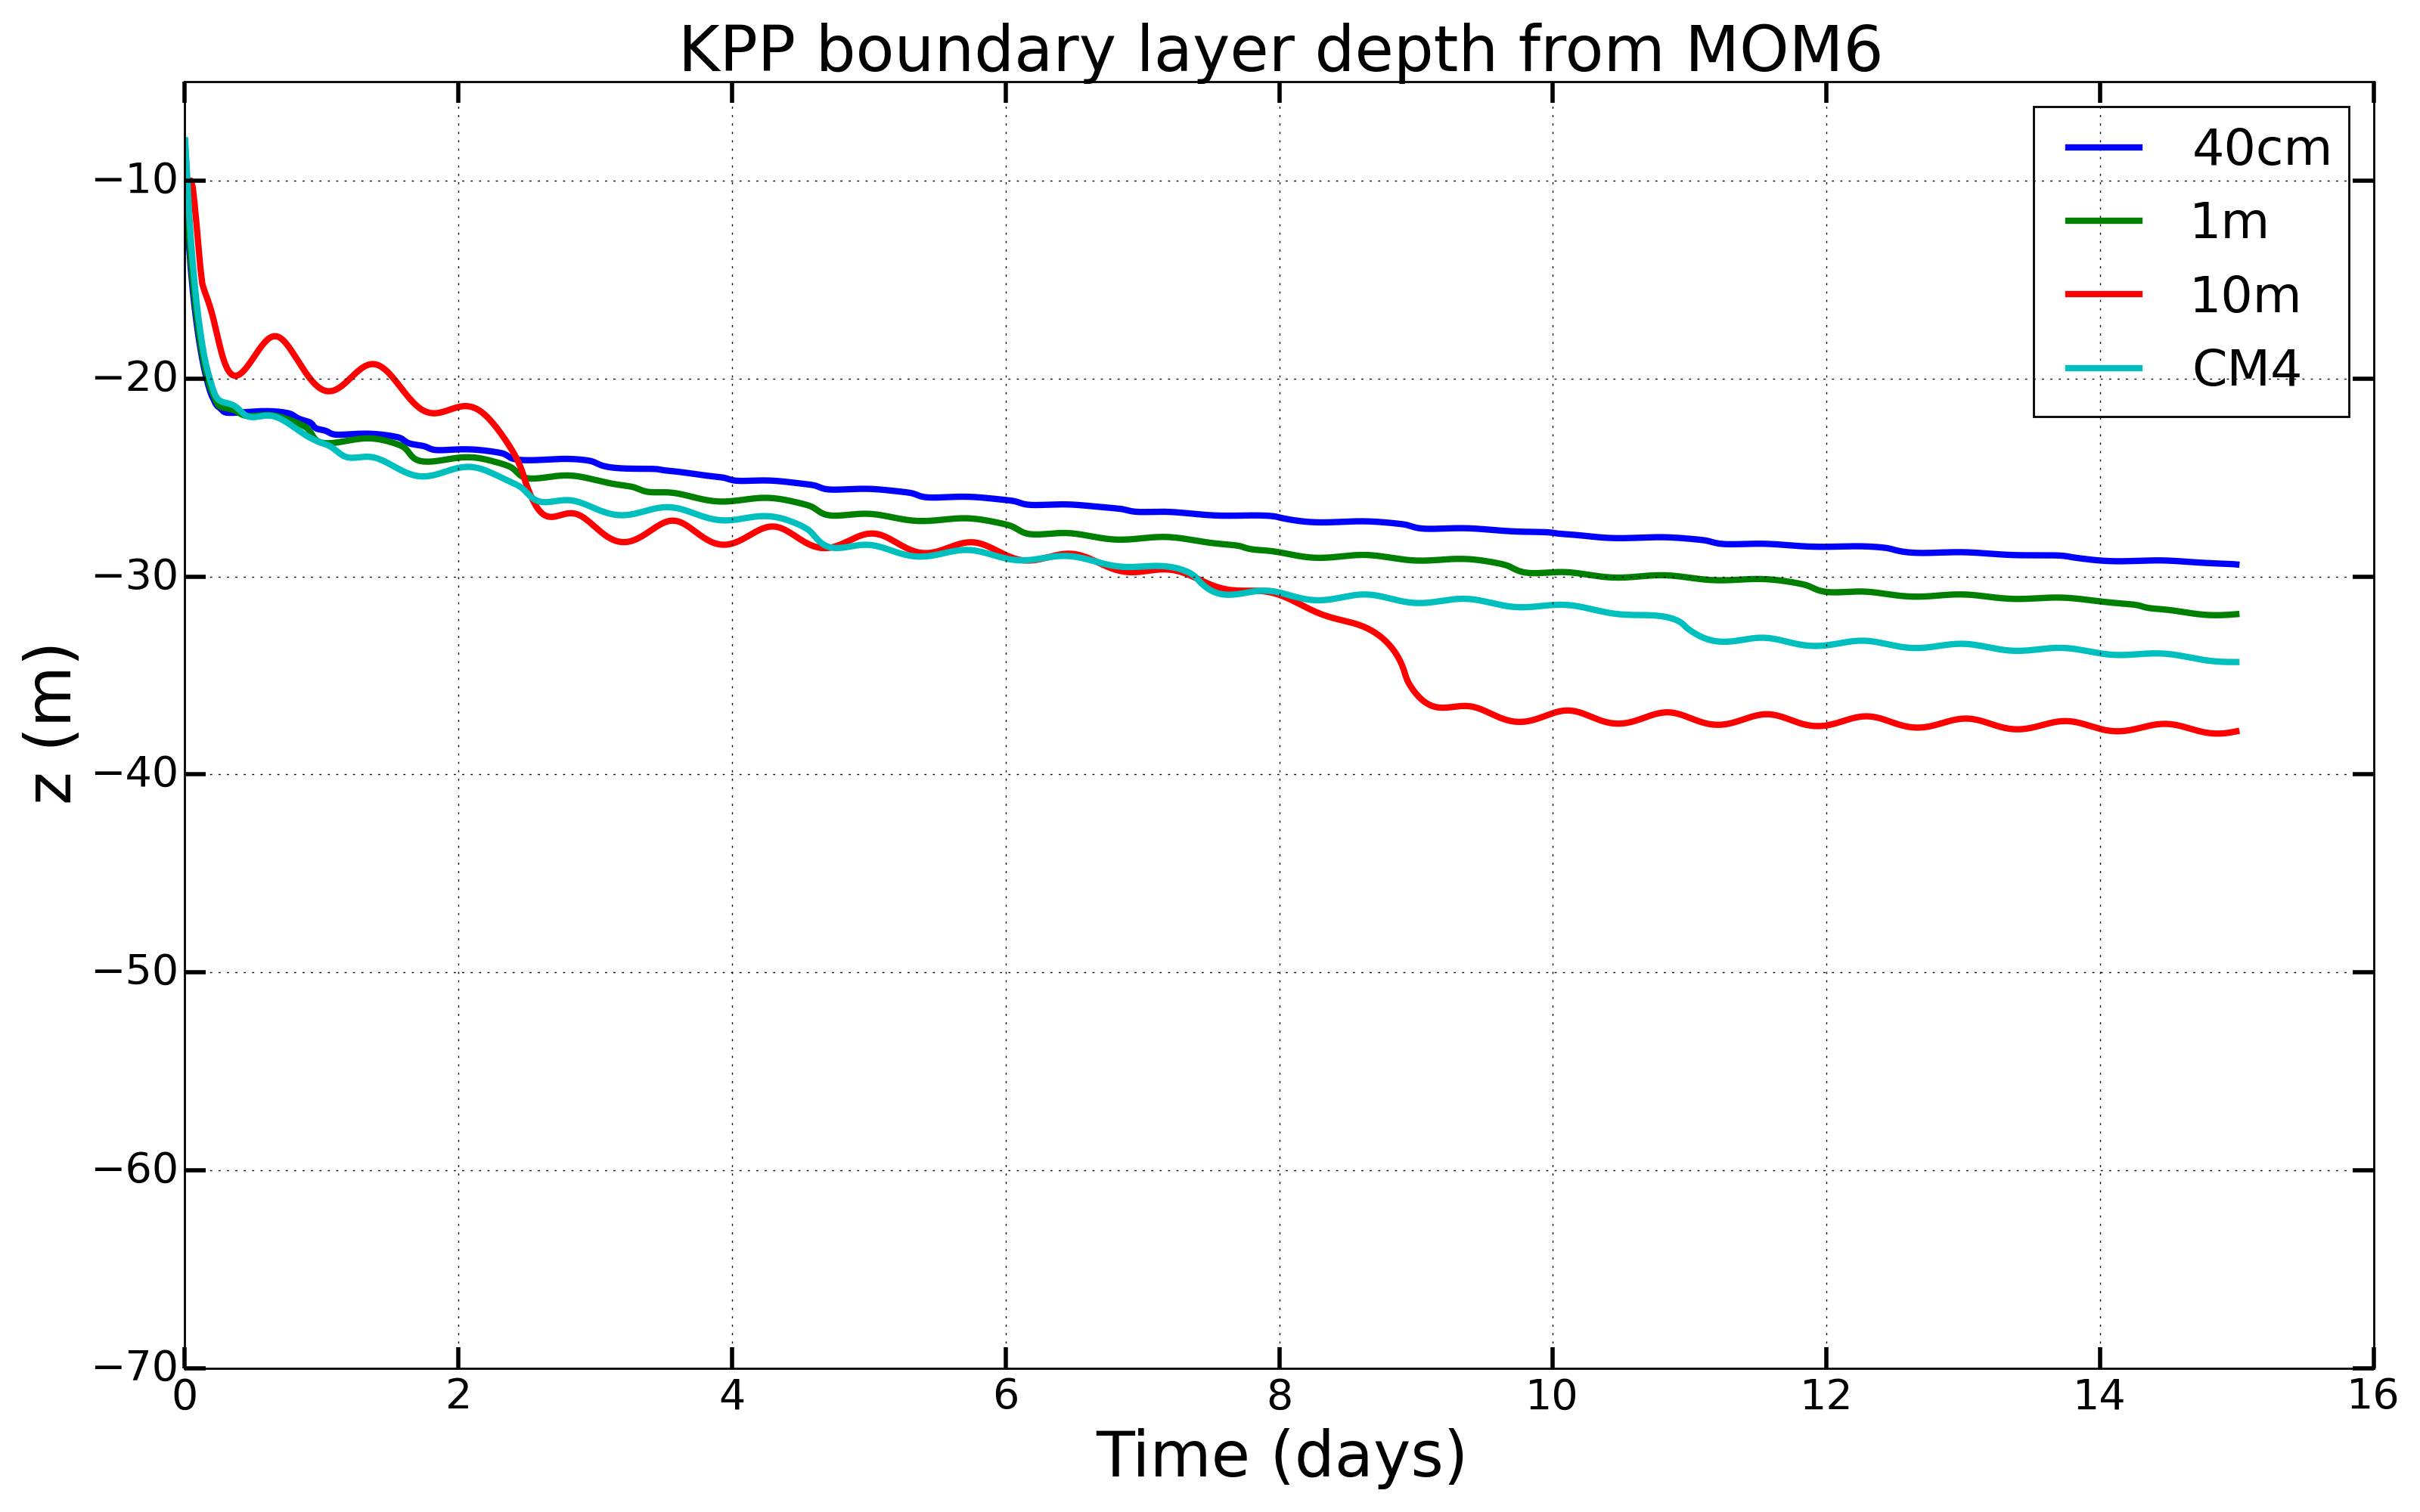
\includegraphics[angle=0,width=5cm]{./figs/MOM6/wind_only_KPP_MOM6_bldepth.png}
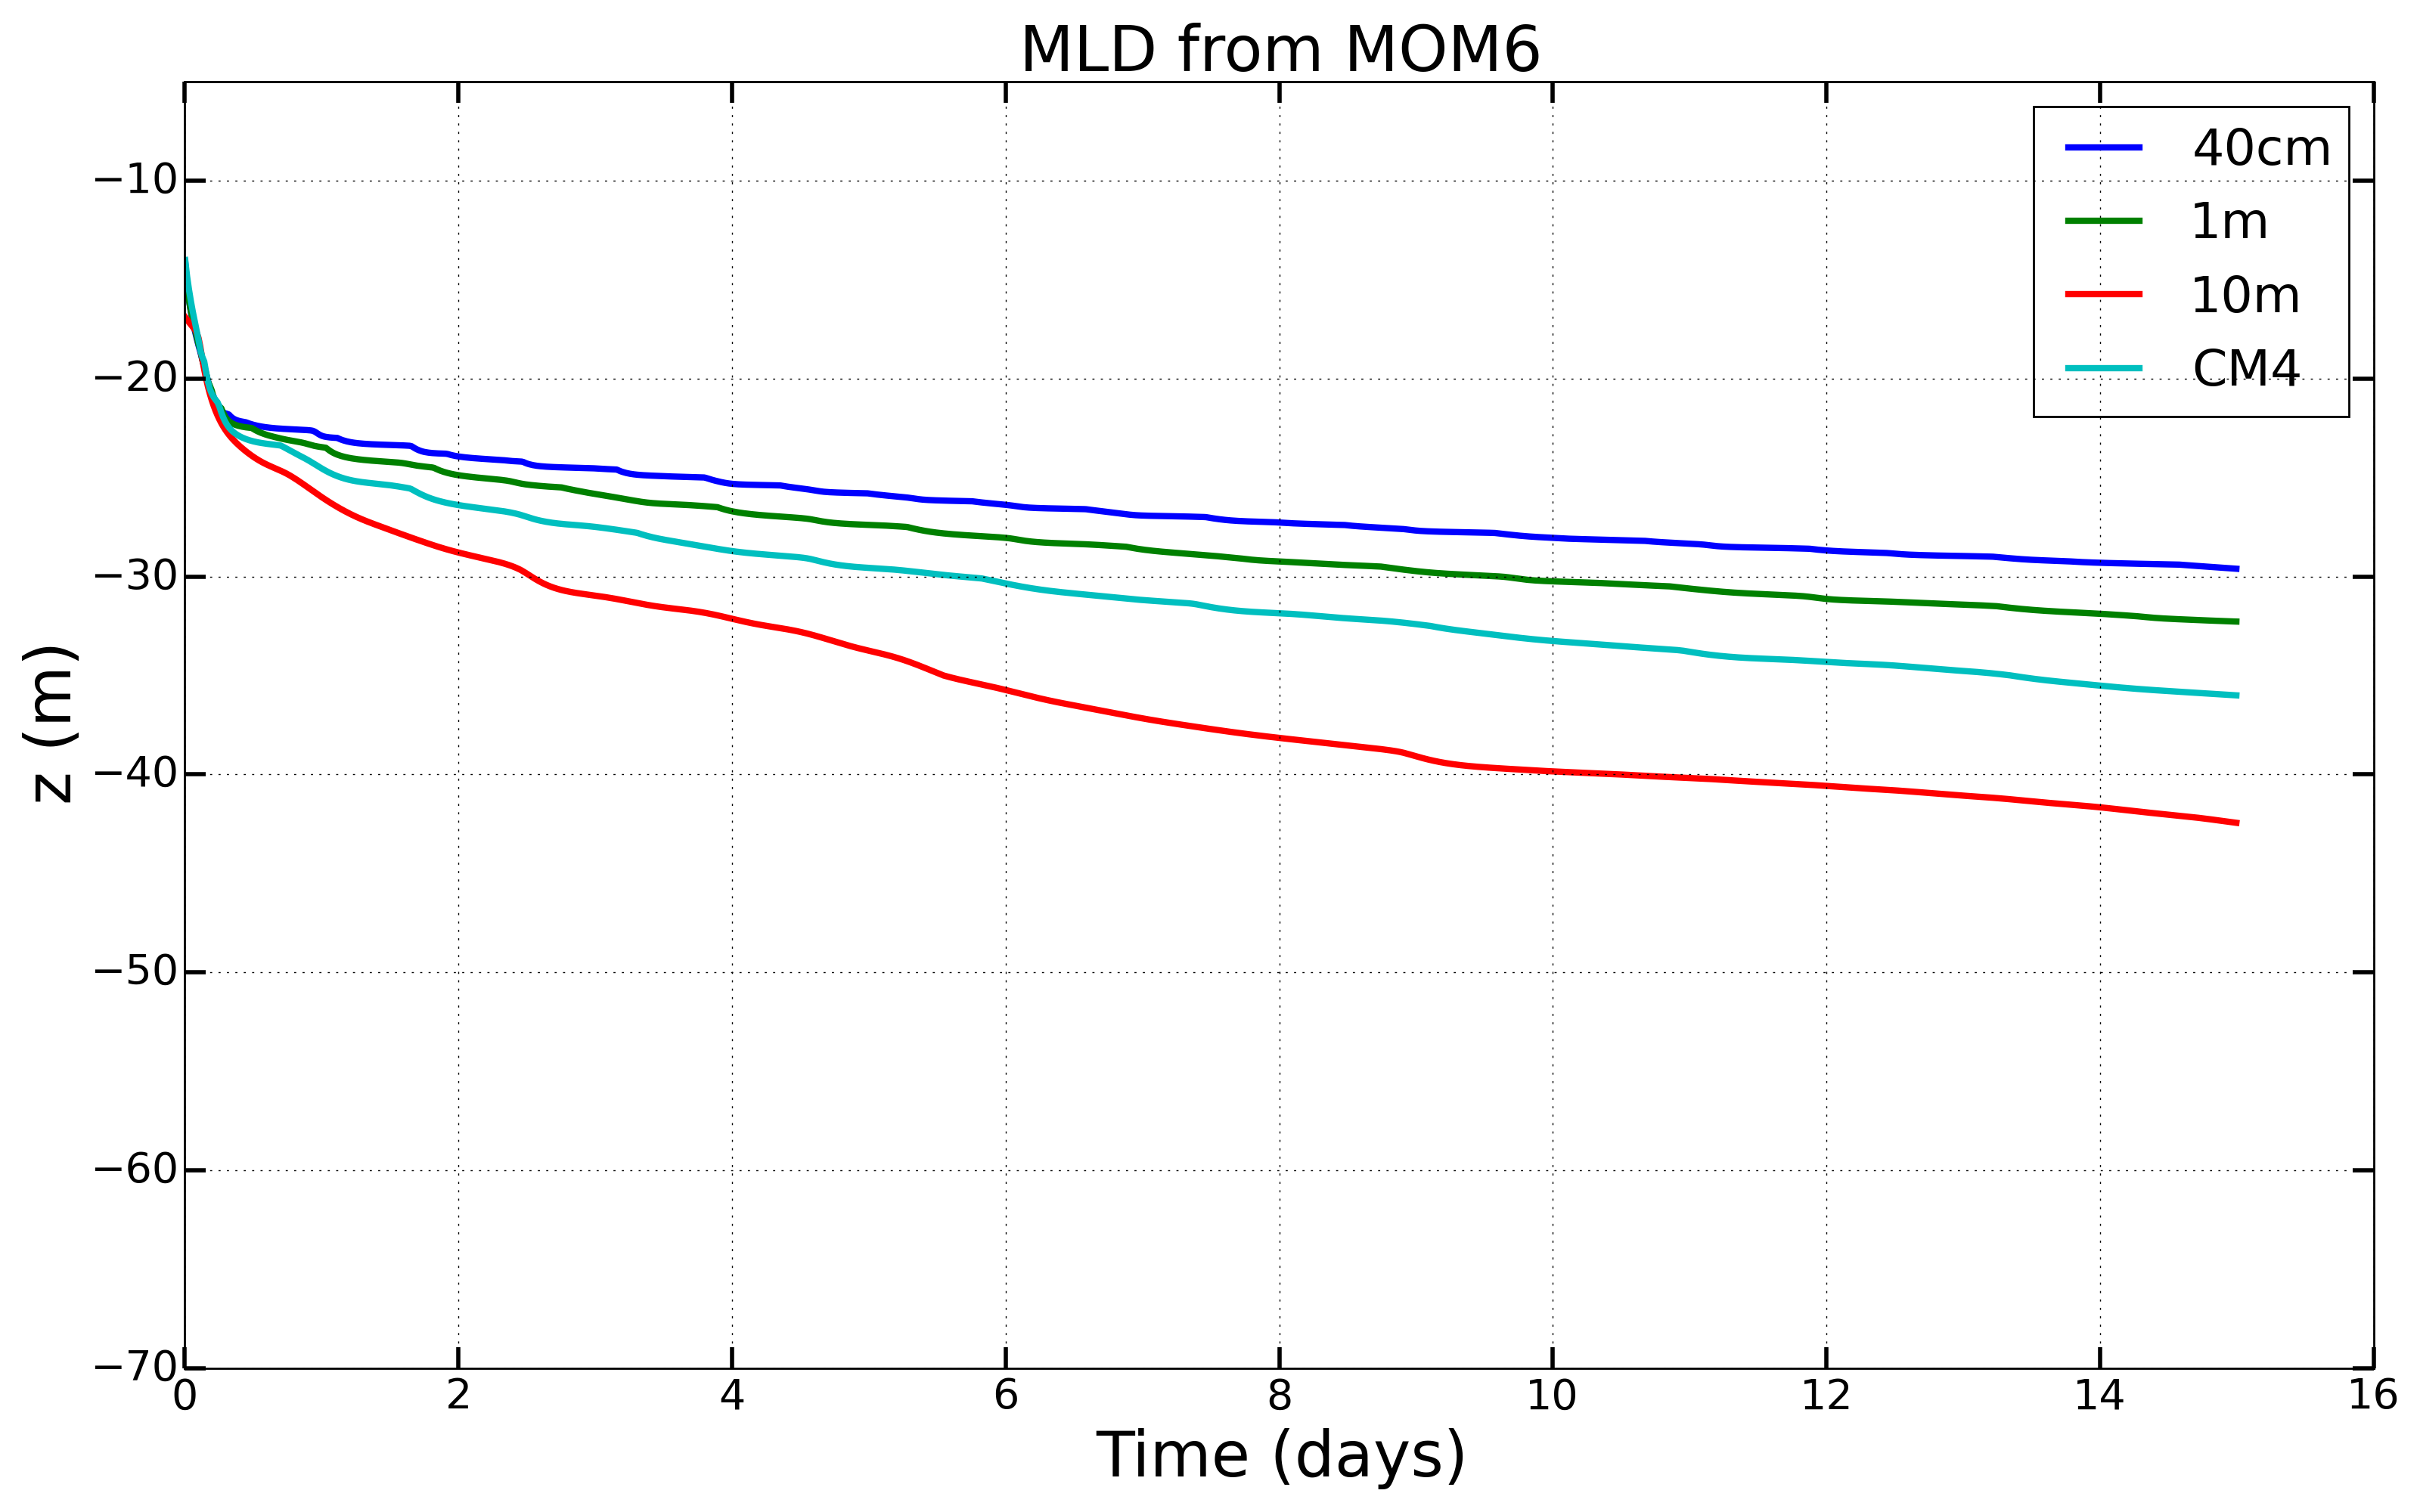
\includegraphics[angle=0,width=5cm]{./figs/MOM6/wind_only_KPP_MOM6_mld.png}
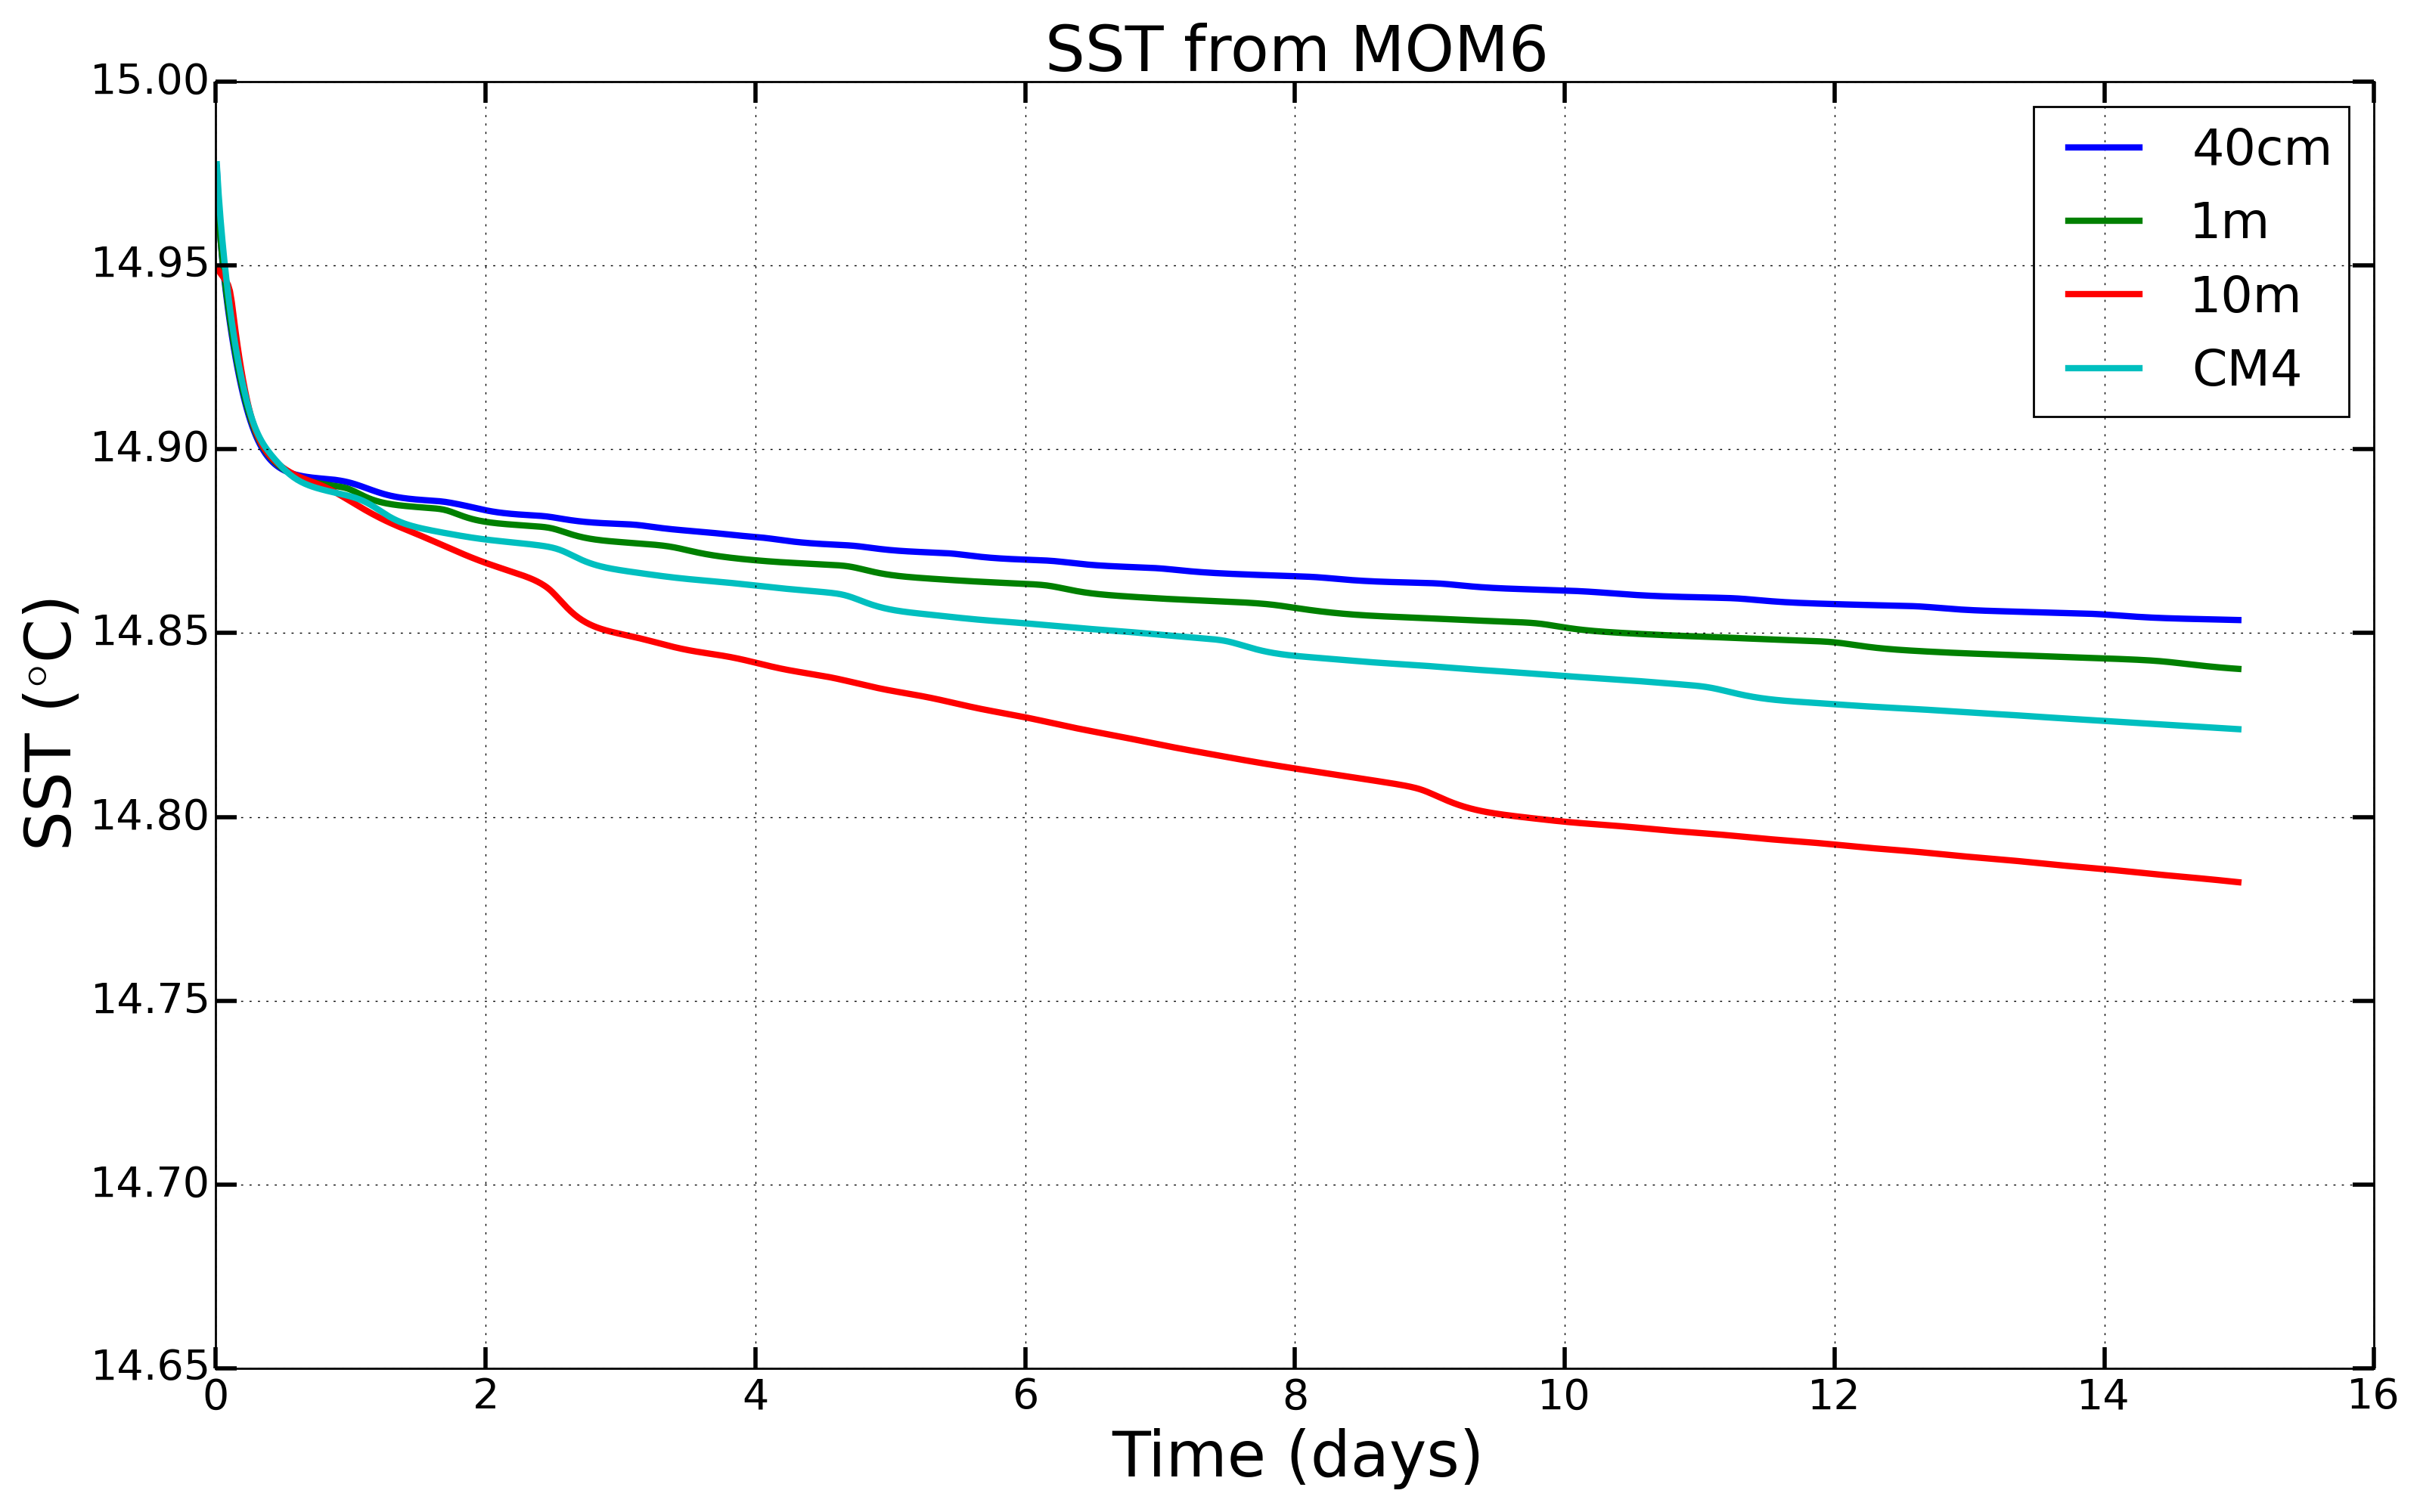
\includegraphics[angle=0,width=5cm]{./figs/MOM6/wind_only_KPP_MOM6_SST.png}
\caption[KPP BL depth, ML depth, and SST from MOM6 for
winds-alone]{\sf Time series for KPP boundary layer depth (left
  panel), mixed layer depth (middle panel), and SST (right panel) for
  the wind test case (constant zonal wind stress and zero surface
  buoyancy forcing) as realized in MOM6.  The mixed layer depth is
  diagnosed as the depth where density differs from the surface by
  $0.003~\mbox{kg}~\mbox{m}^{-3}.$}
\label{fig:MOM6_SST_bldepth-wind_alone}
\end{center}
%\rule{\textwidth}{0.005in}
\end{figure}
%%%%%%%%%%%%%%%%%%%%%%%%%%%%%%%%%%%%%%%%%%%%%%%%%%%%%%%%%%%%%%%%%%%%%%%%


%%%%%%%%%%%%%%%%%%%% %%%%%%%%%%%%%%%%%%%%%%%%%
\begin{figure}[h!t]
%\rule{\textwidth}{0.005in}
\begin{center}
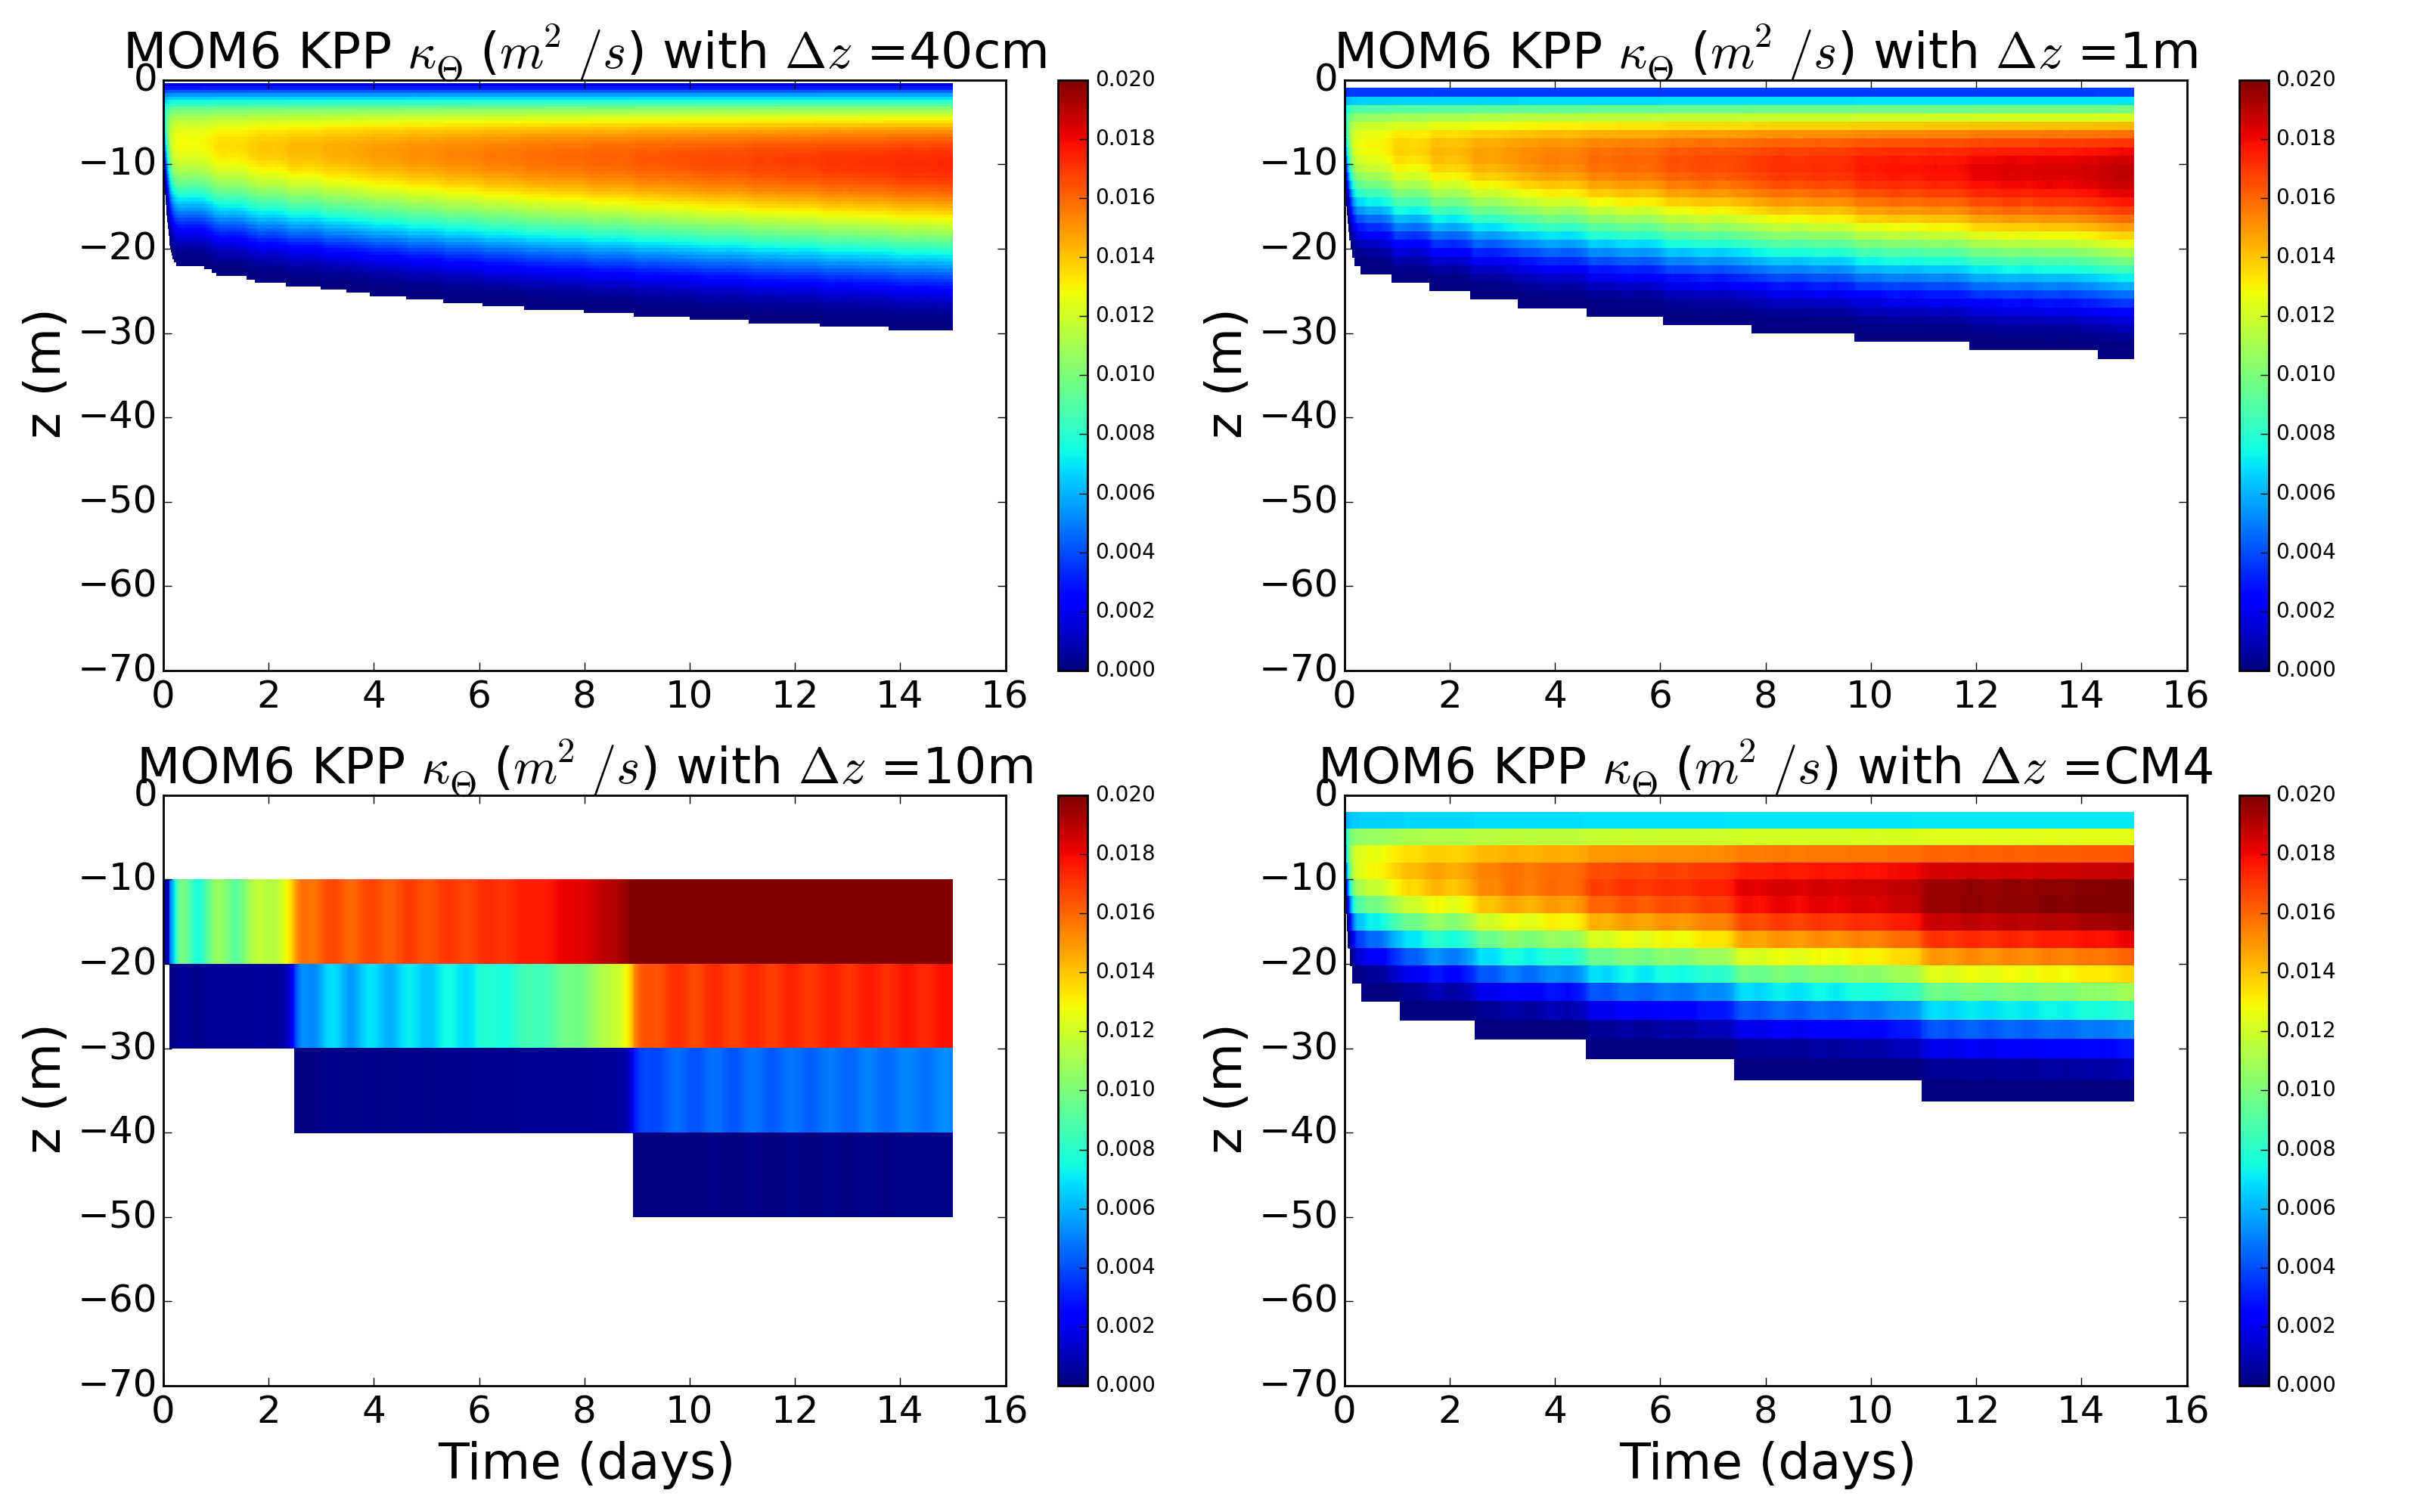
\includegraphics[angle=0,width=14cm]{./figs/MOM6/wind_only_KPP_MOM6_KPP_diffusivity.png}
\caption[KPP diffusivity from MOM6 for winds-alone test]{\sf Time
  series for the KPP vertical diffusivity for the wind test case
  (constant zonal wind stress and zero surface buoyancy forcing) as
  realized in MOM6 using four different vertical grid resolutions.
  The diffusivity is centered on the bottom interface of a grid cell,
  with the first nonzero value at the bottom of the surface cell.}
\label{fig:MOM6_KPP_diffusivity-wind_alone}
\end{center}
%\rule{\textwidth}{0.005in}
\end{figure}
%%%%%%%%%%%%%%%%%%%%%%%%%%%%%%%%%%%%%%%%%%%%%%%%%%%%%%%%%%%%%%%%%%%%%%%%


%%%%%%%%%%%%%%%%%%%% %%%%%%%%%%%%%%%%%%%%%%%%%
\begin{figure}[h!t]
%\rule{\textwidth}{0.005in}
\begin{center}
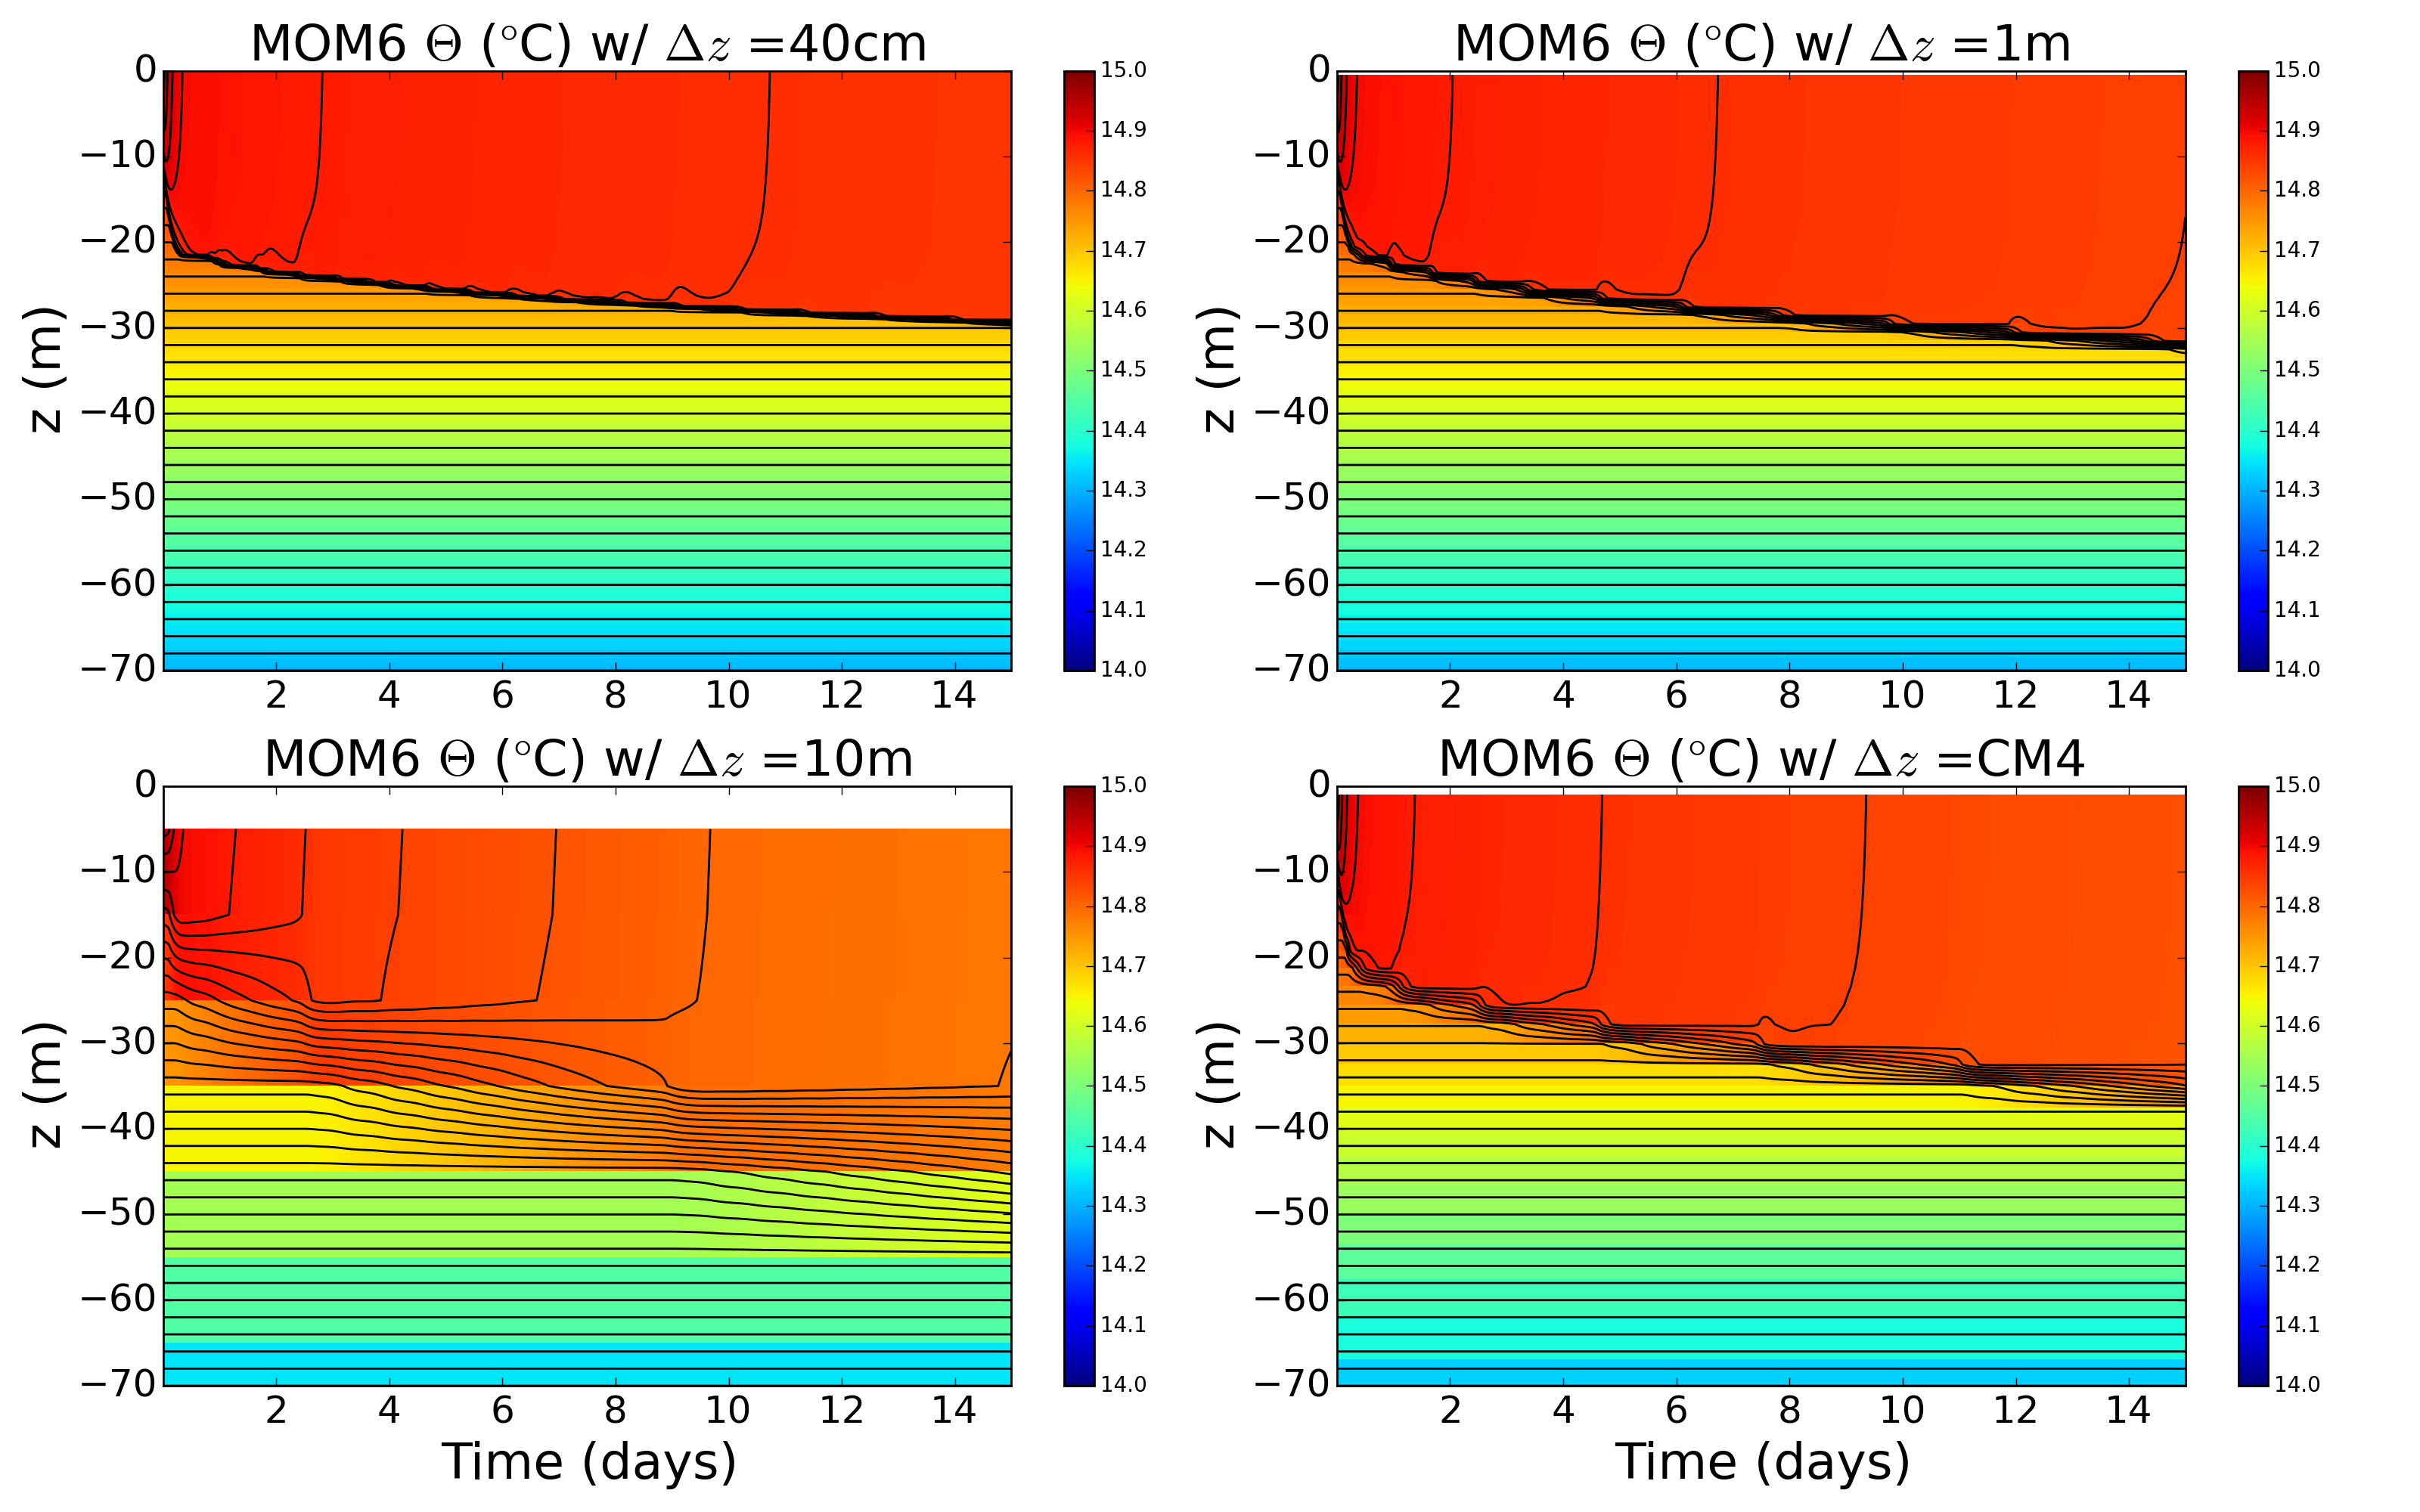
\includegraphics[angle=0,width=14cm]{./figs/MOM6/wind_only_KPP_MOM6_temp.png}
\caption[Temperature from MOM6 for winds-alone test]{\sf Time series
  for temperature in the wind test case (constant zonal wind stress
  and zero surface buoyancy forcing) as realized in MOM6 using four
  different vertical grid resolutions.  The temperature is located at
  the center of a grid cell, with the first nonzero value at the
  center of the surface cell.}
\label{fig:MOM6_temp-wind_alone}
\end{center}
%\rule{\textwidth}{0.005in}
\end{figure}
%%%%%%%%%%%%%%%%%%%%%%%%%%%%%%%%%%%%%%%%%%%%%%%%%%%%%%%%%%%%%%%%%%%%%%%%

%%%%%%%%%%%%%%%%%%%% %%%%%%%%%%%%%%%%%%%%%%%%%
\begin{figure}[h!t]
%\rule{\textwidth}{0.005in}
\begin{center}
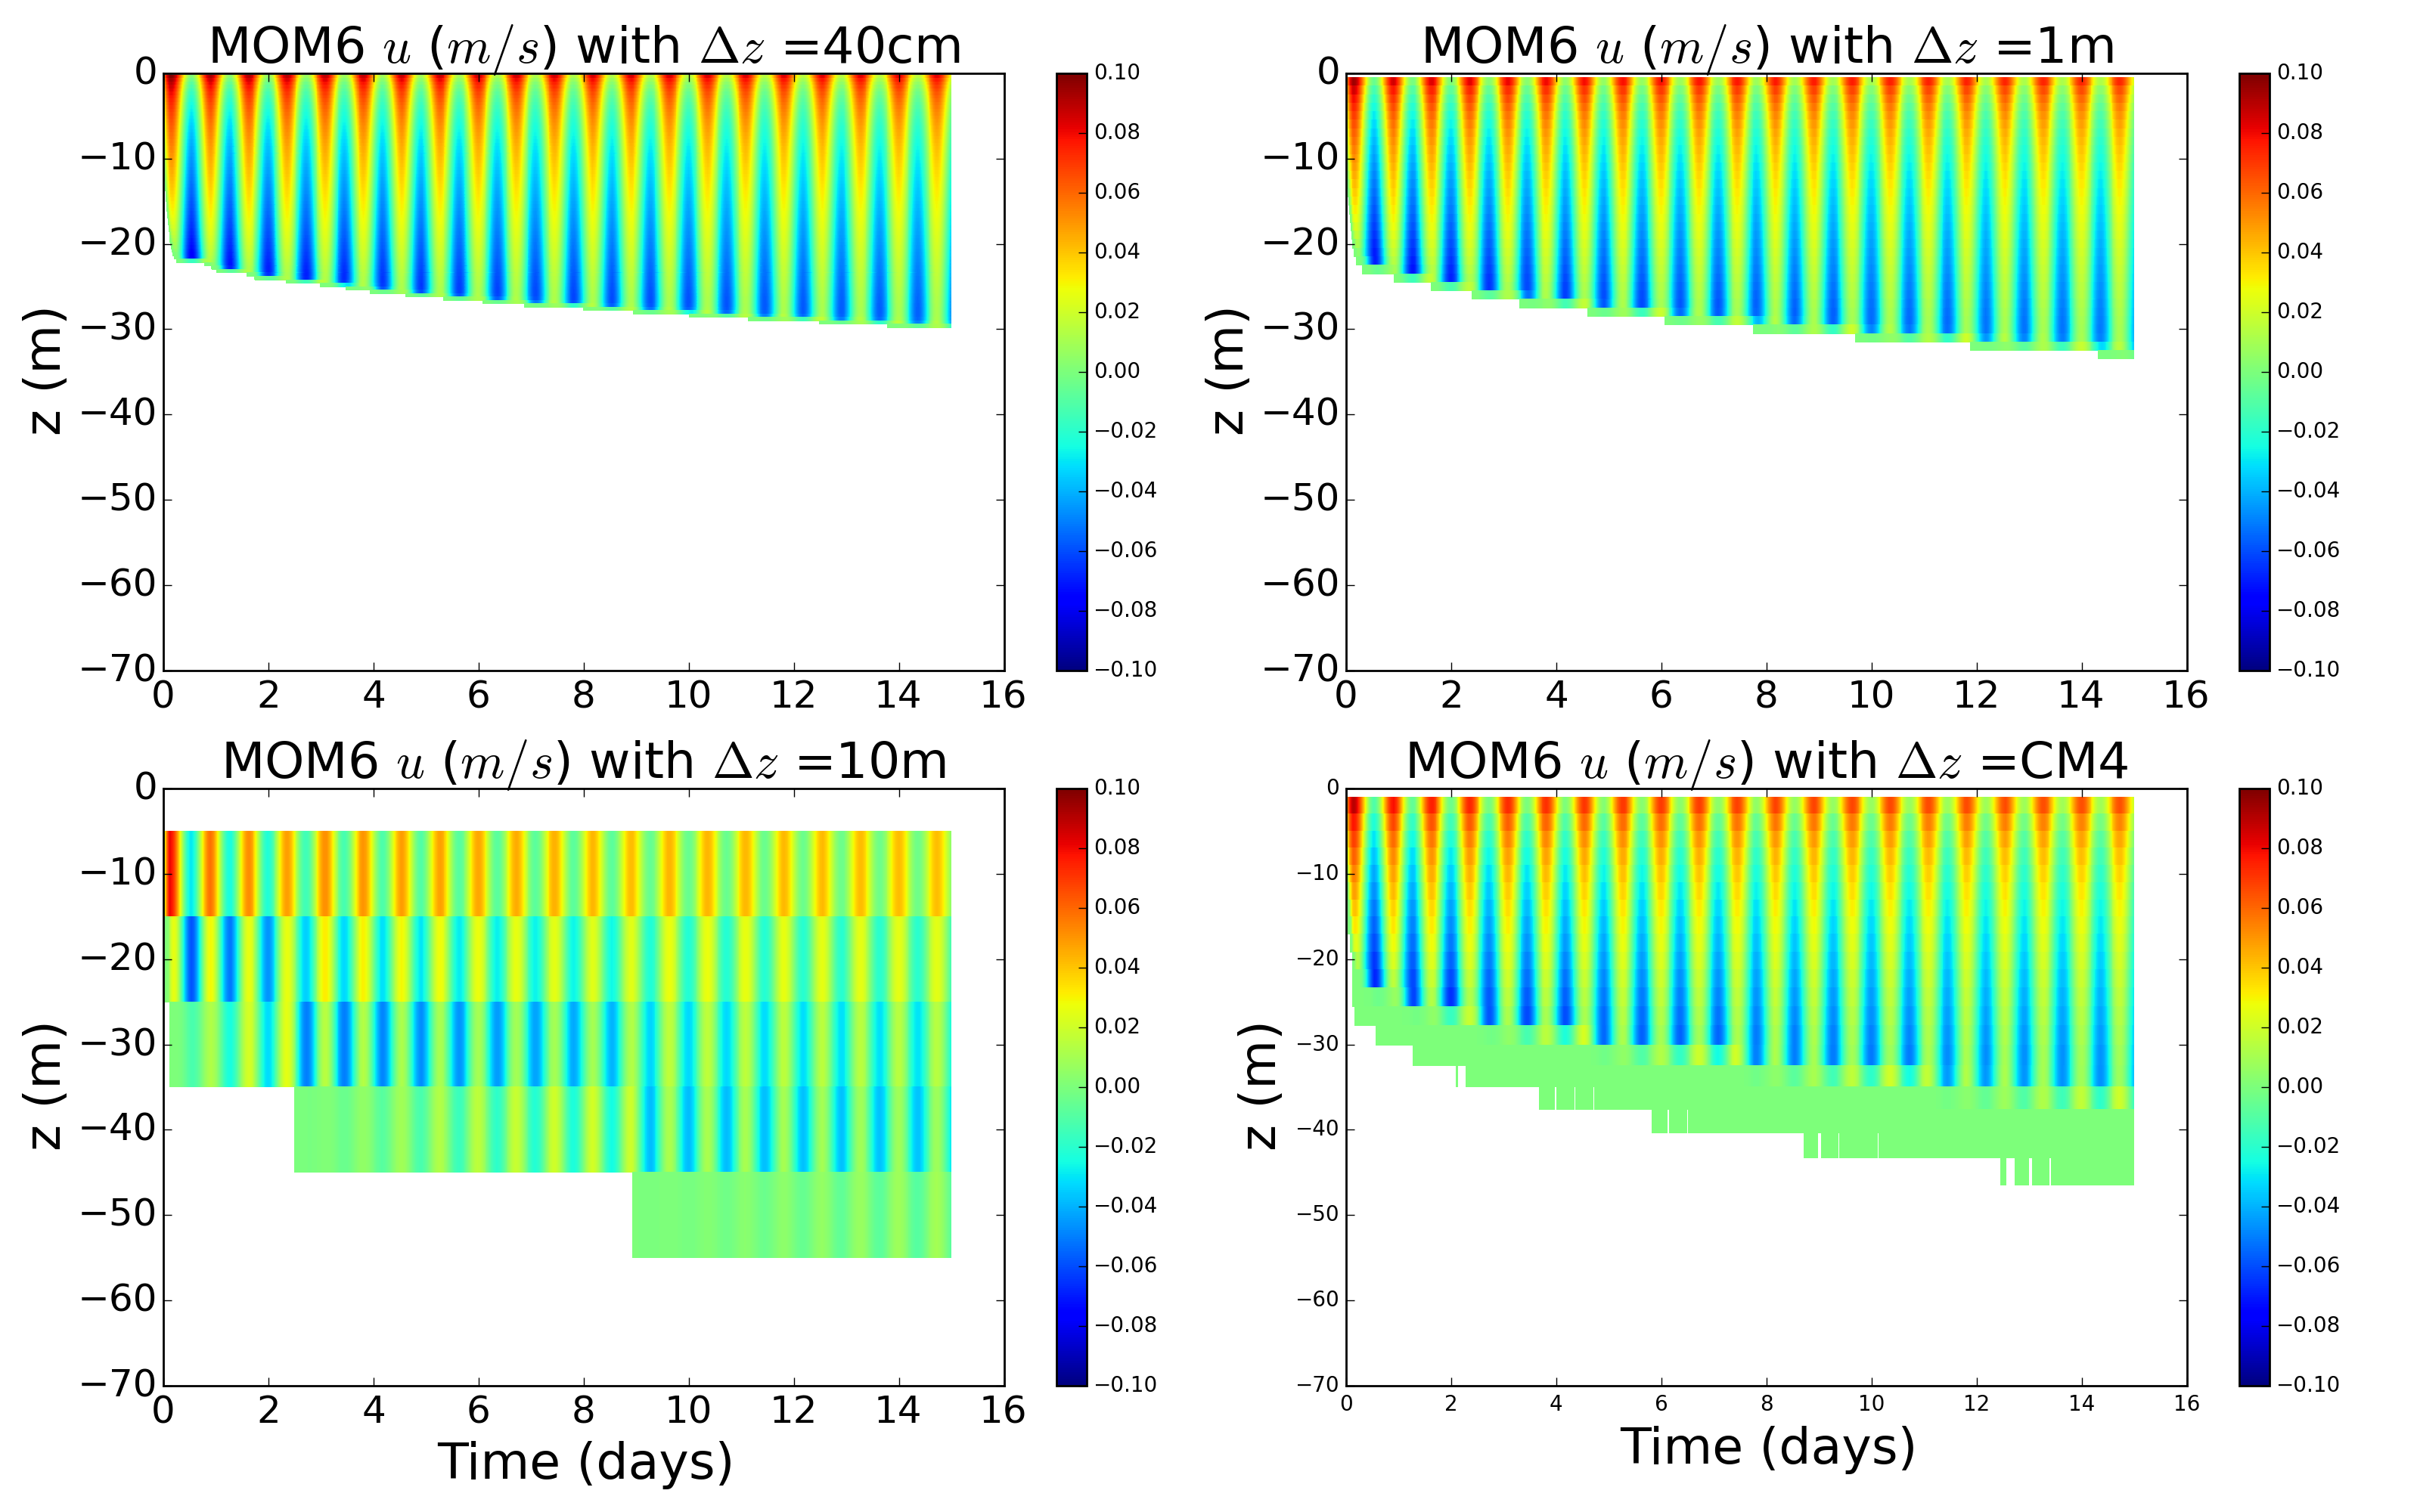
\includegraphics[angle=0,width=14cm]{./figs/MOM6/wind_only_KPP_MOM6_zonal_velocity.png}
\caption[Zonal velocity from MOM6 for winds-alone test]{\sf Time
  series for zonal velocity in the wind test case (constant zonal wind
  stress and zero surface buoyancy forcing) as realized in MOM6 using
  four different vertical grid resolutions. The velocity is centered
  on the center of a grid cell, with the first nonzero value at the
  center of the surface cell.}
\label{fig:MOM6_zonal-wind_alone}
\end{center}
%\rule{\textwidth}{0.005in}
\end{figure}
%%%%%%%%%%%%%%%%%%%%%%%%%%%%%%%%%%%%%%%%%%%%%%%%%%%%%%%%%%%%%%%%%%%%%%%%






\chapter{Wind stress plus heating}
\label{chapter:winds_and_heating}

In this chapter, we document a test configured with a constant zonal
wind stress
\begin{equation}
 \bftau  =  (0.1, 0)~\mbox{N}~\mbox{m}^{-2}
\end{equation}
plus a constant positive heat flux applied in the top grid cell
\begin{equation}
Q=100~\mbox{W}~\mbox{m}^{-2}.
\end{equation}
The temperature is initialized with uniform value of
$15^{\circ}~\mbox{C}$.  In this experiment, the positive buoyancy
applied to the surface grid cell is mixed downward by the mechanical
forcing by wind stress.  This process develops a nonzero
stratification at depth, with the depth determined by the wind stress.
The non-local KPP term vanishes since the buoyancy flux is positive.



\minitoc


\section{Results from GFDL-MOM6}
\label{section:wind_and_heating_mom6}

Figure \ref{fig:MOM6_SST_bldepth-wind_and_heating} shows the KPP
boundary layer depth from the MOM6 implementation of CVMix/KPP.
Within a couple of days, the boundary layer rapidly reaches a near
stationary value.  The coarsest grid, $\Delta z = 10~\mbox{m}$, has
the shallowest boundary layer just deeper than $15~\mbox{m}$, whereas
the other three grids are deeper than $25~\mbox{m}$.  The mixed layer
depth tracks very close to the boundary layer depth for this test
case.  The SST exhibits a steady increase for all grids, with the
$\Delta z = 10~\mbox{m}$ test warming the most given that its e
boundary layer is shallowest, thus trapping more of the surface
heating in the top grid cell.

The KPP diffusivity is shown in Figure
\ref{fig:MOM6_KPP_diffusivity-wind_and_heating}, with each grid
showing the same characteristics of an initially large value settling
down within a day to nearly steady values.  Diffusivity in the $\Delta
z = 10~\mbox{m}$ grid is smallest since the boundary layer depth is
smallest in this simulation.  In fact, the boundary layer for this
grid occupies only two grid cells, which is arguably under-resolved.
  
Figure \ref{fig:MOM6_temp-wind_and_heating} shows impacts of the upper
ocean heating and wind stress on the depth profile of temperature,
whereas Figure \ref{fig:MOM6_zonal-wind_and_heating} exhibits the
inertial oscillations in zonal velocity associated with the zonal wind
stress.  

%%%%%%%%%%%%%%%%%%%% %%%%%%%%%%%%%%%%%%%%%%%%%
\begin{figure}[h!t]
%\rule{\textwidth}{0.005in}
\begin{center}
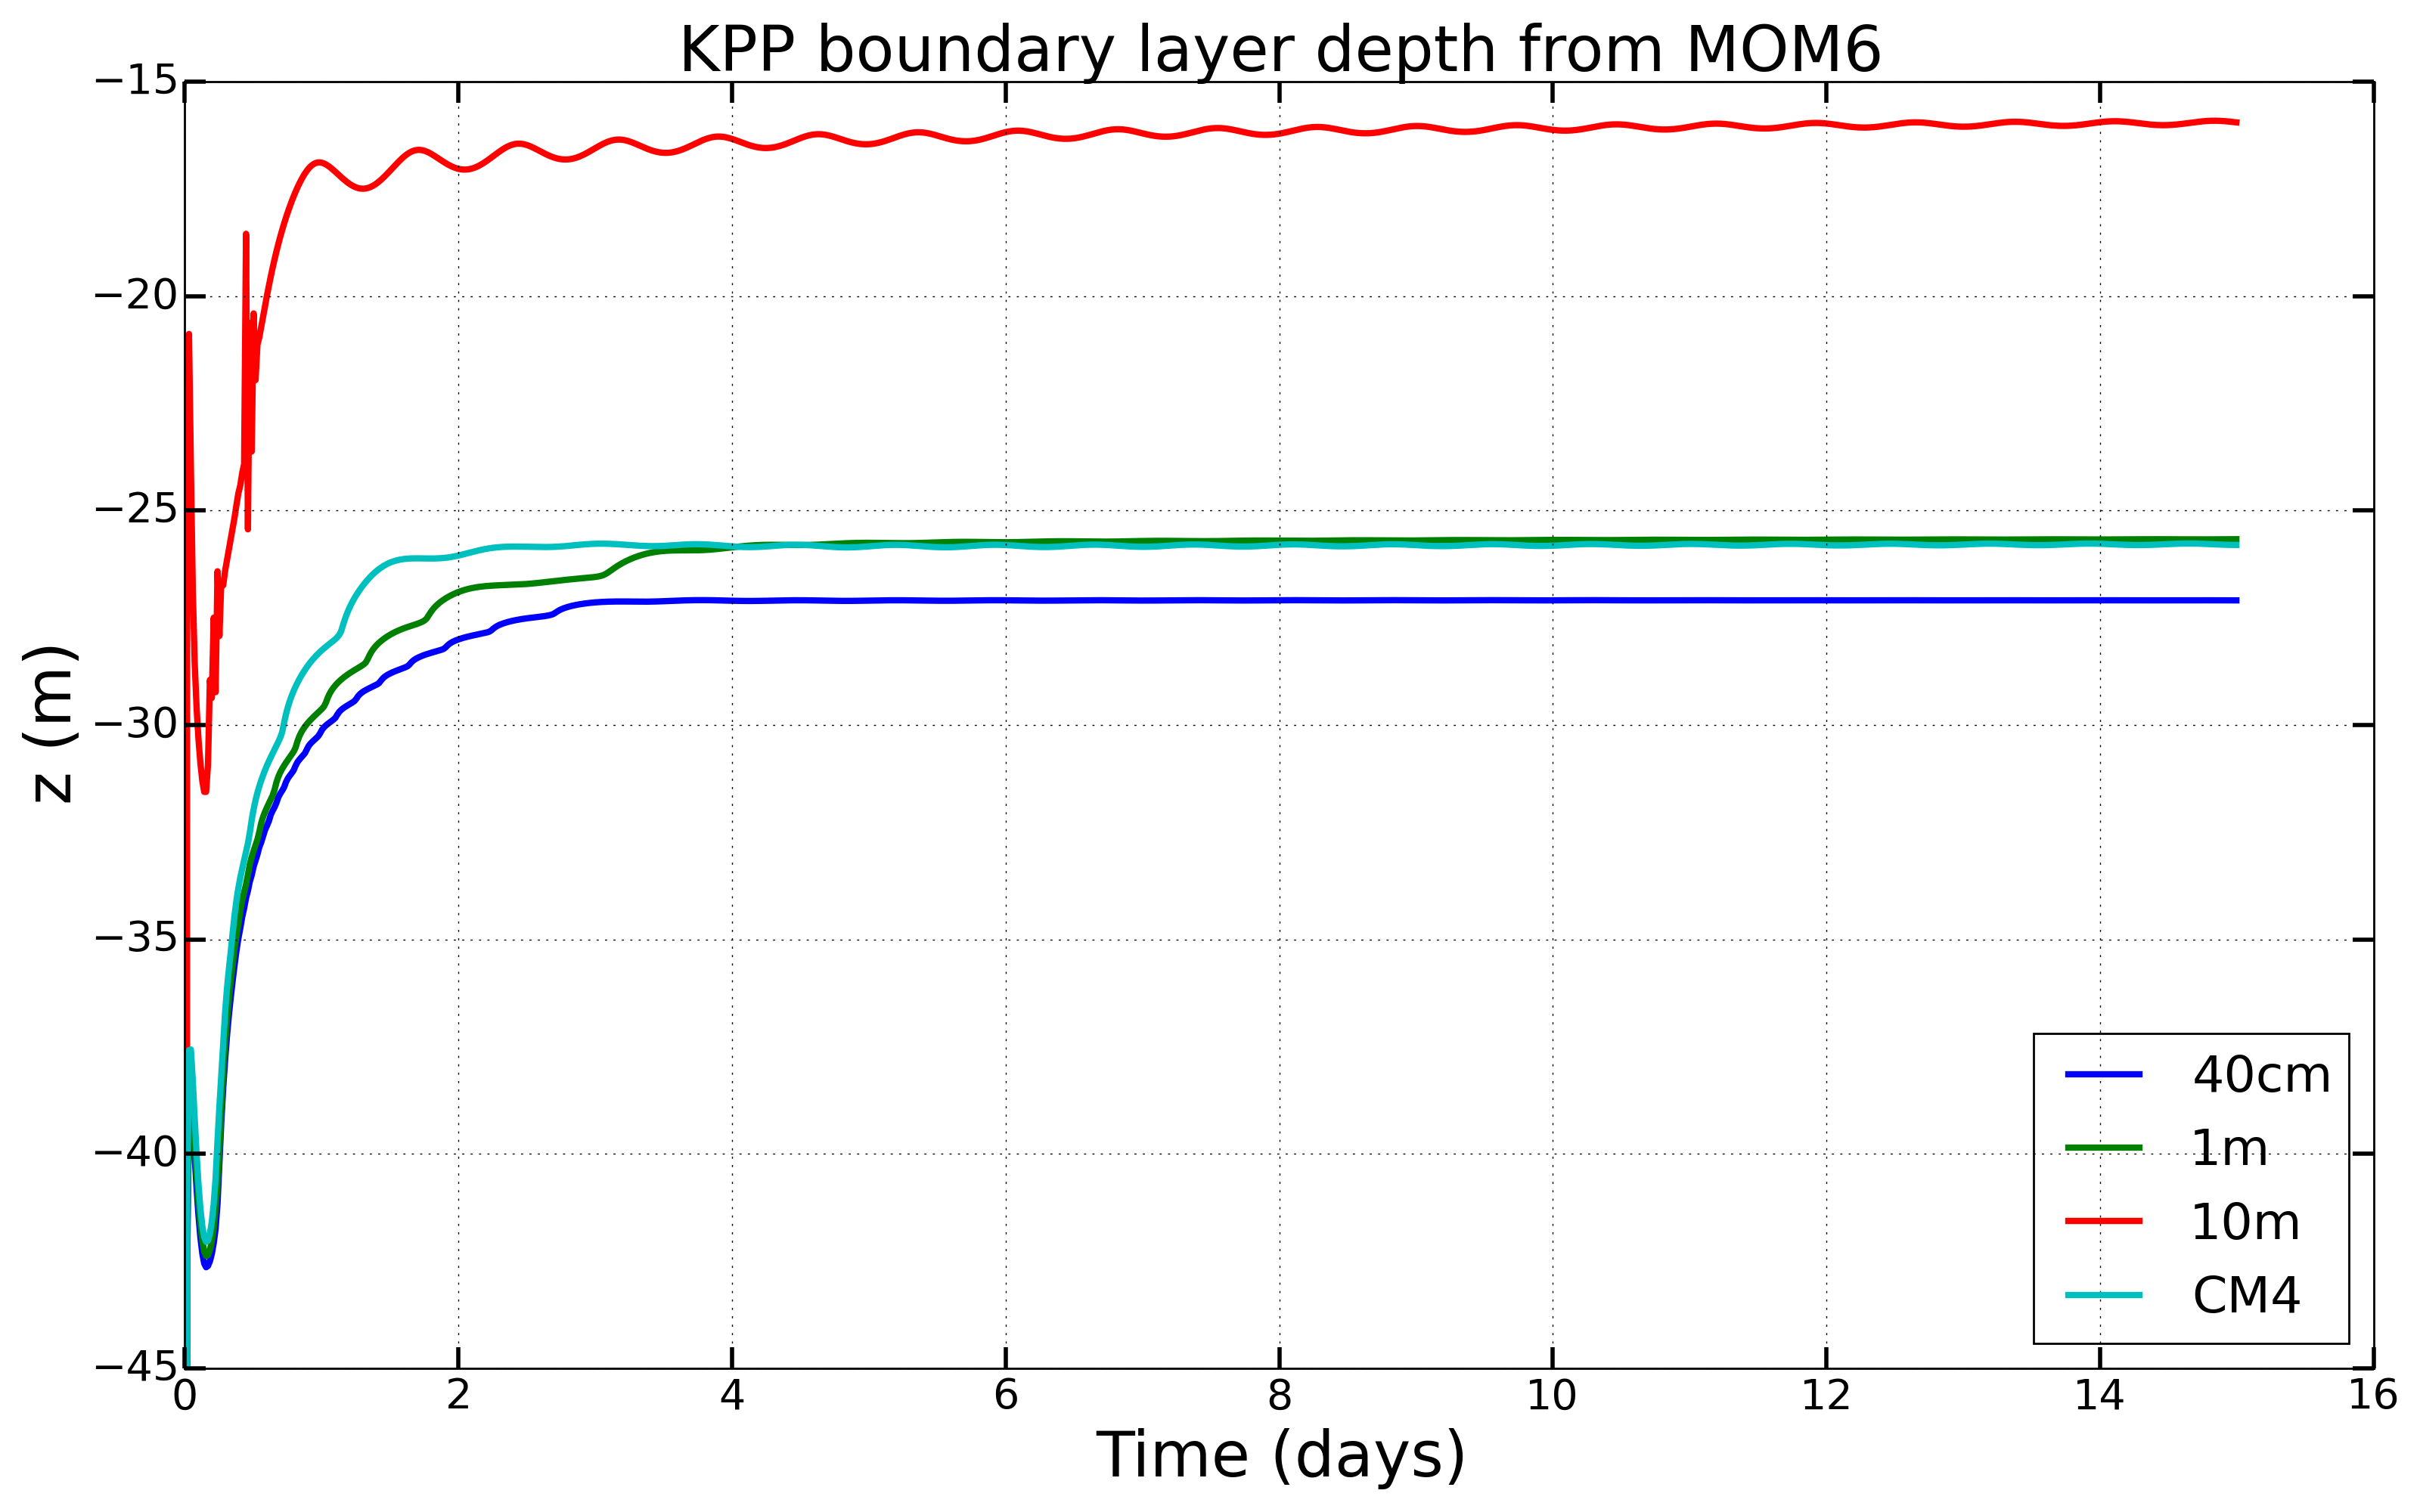
\includegraphics[angle=0,width=5cm]{./figs/MOM6/skin_warming_wind_KPP_MOM6_bldepth.png}
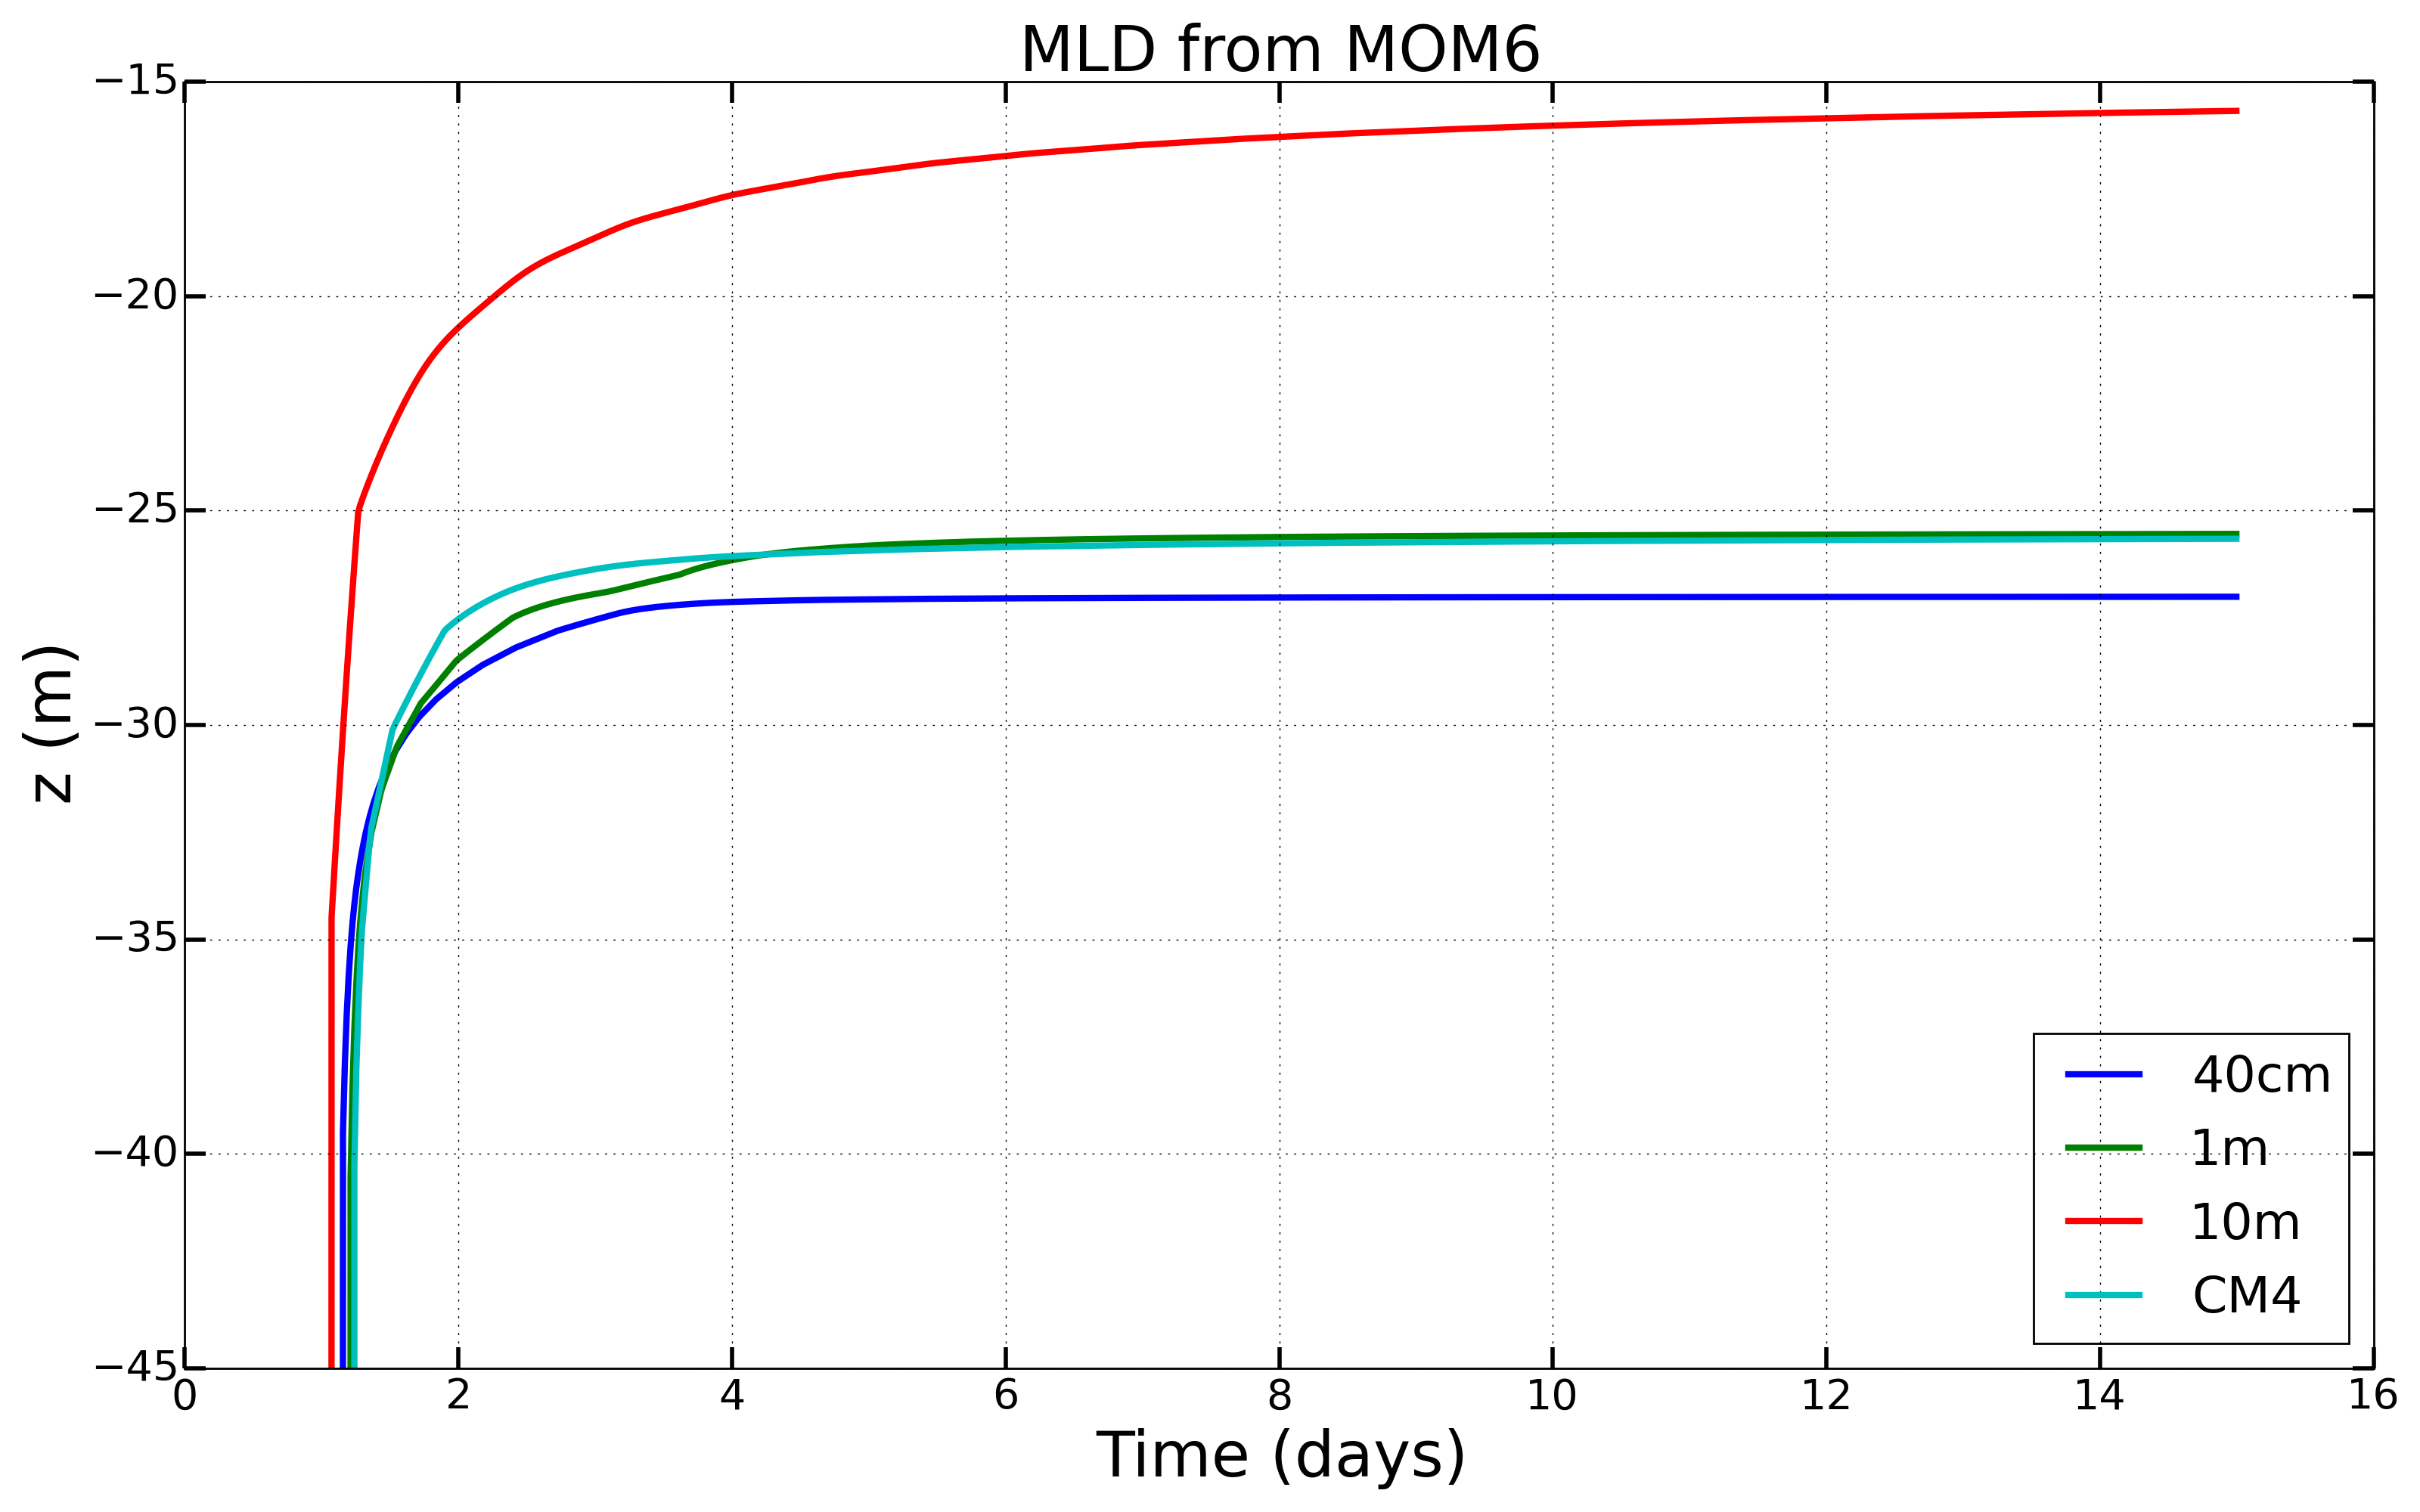
\includegraphics[angle=0,width=5cm]{./figs/MOM6/skin_warming_wind_KPP_MOM6_mld.png}
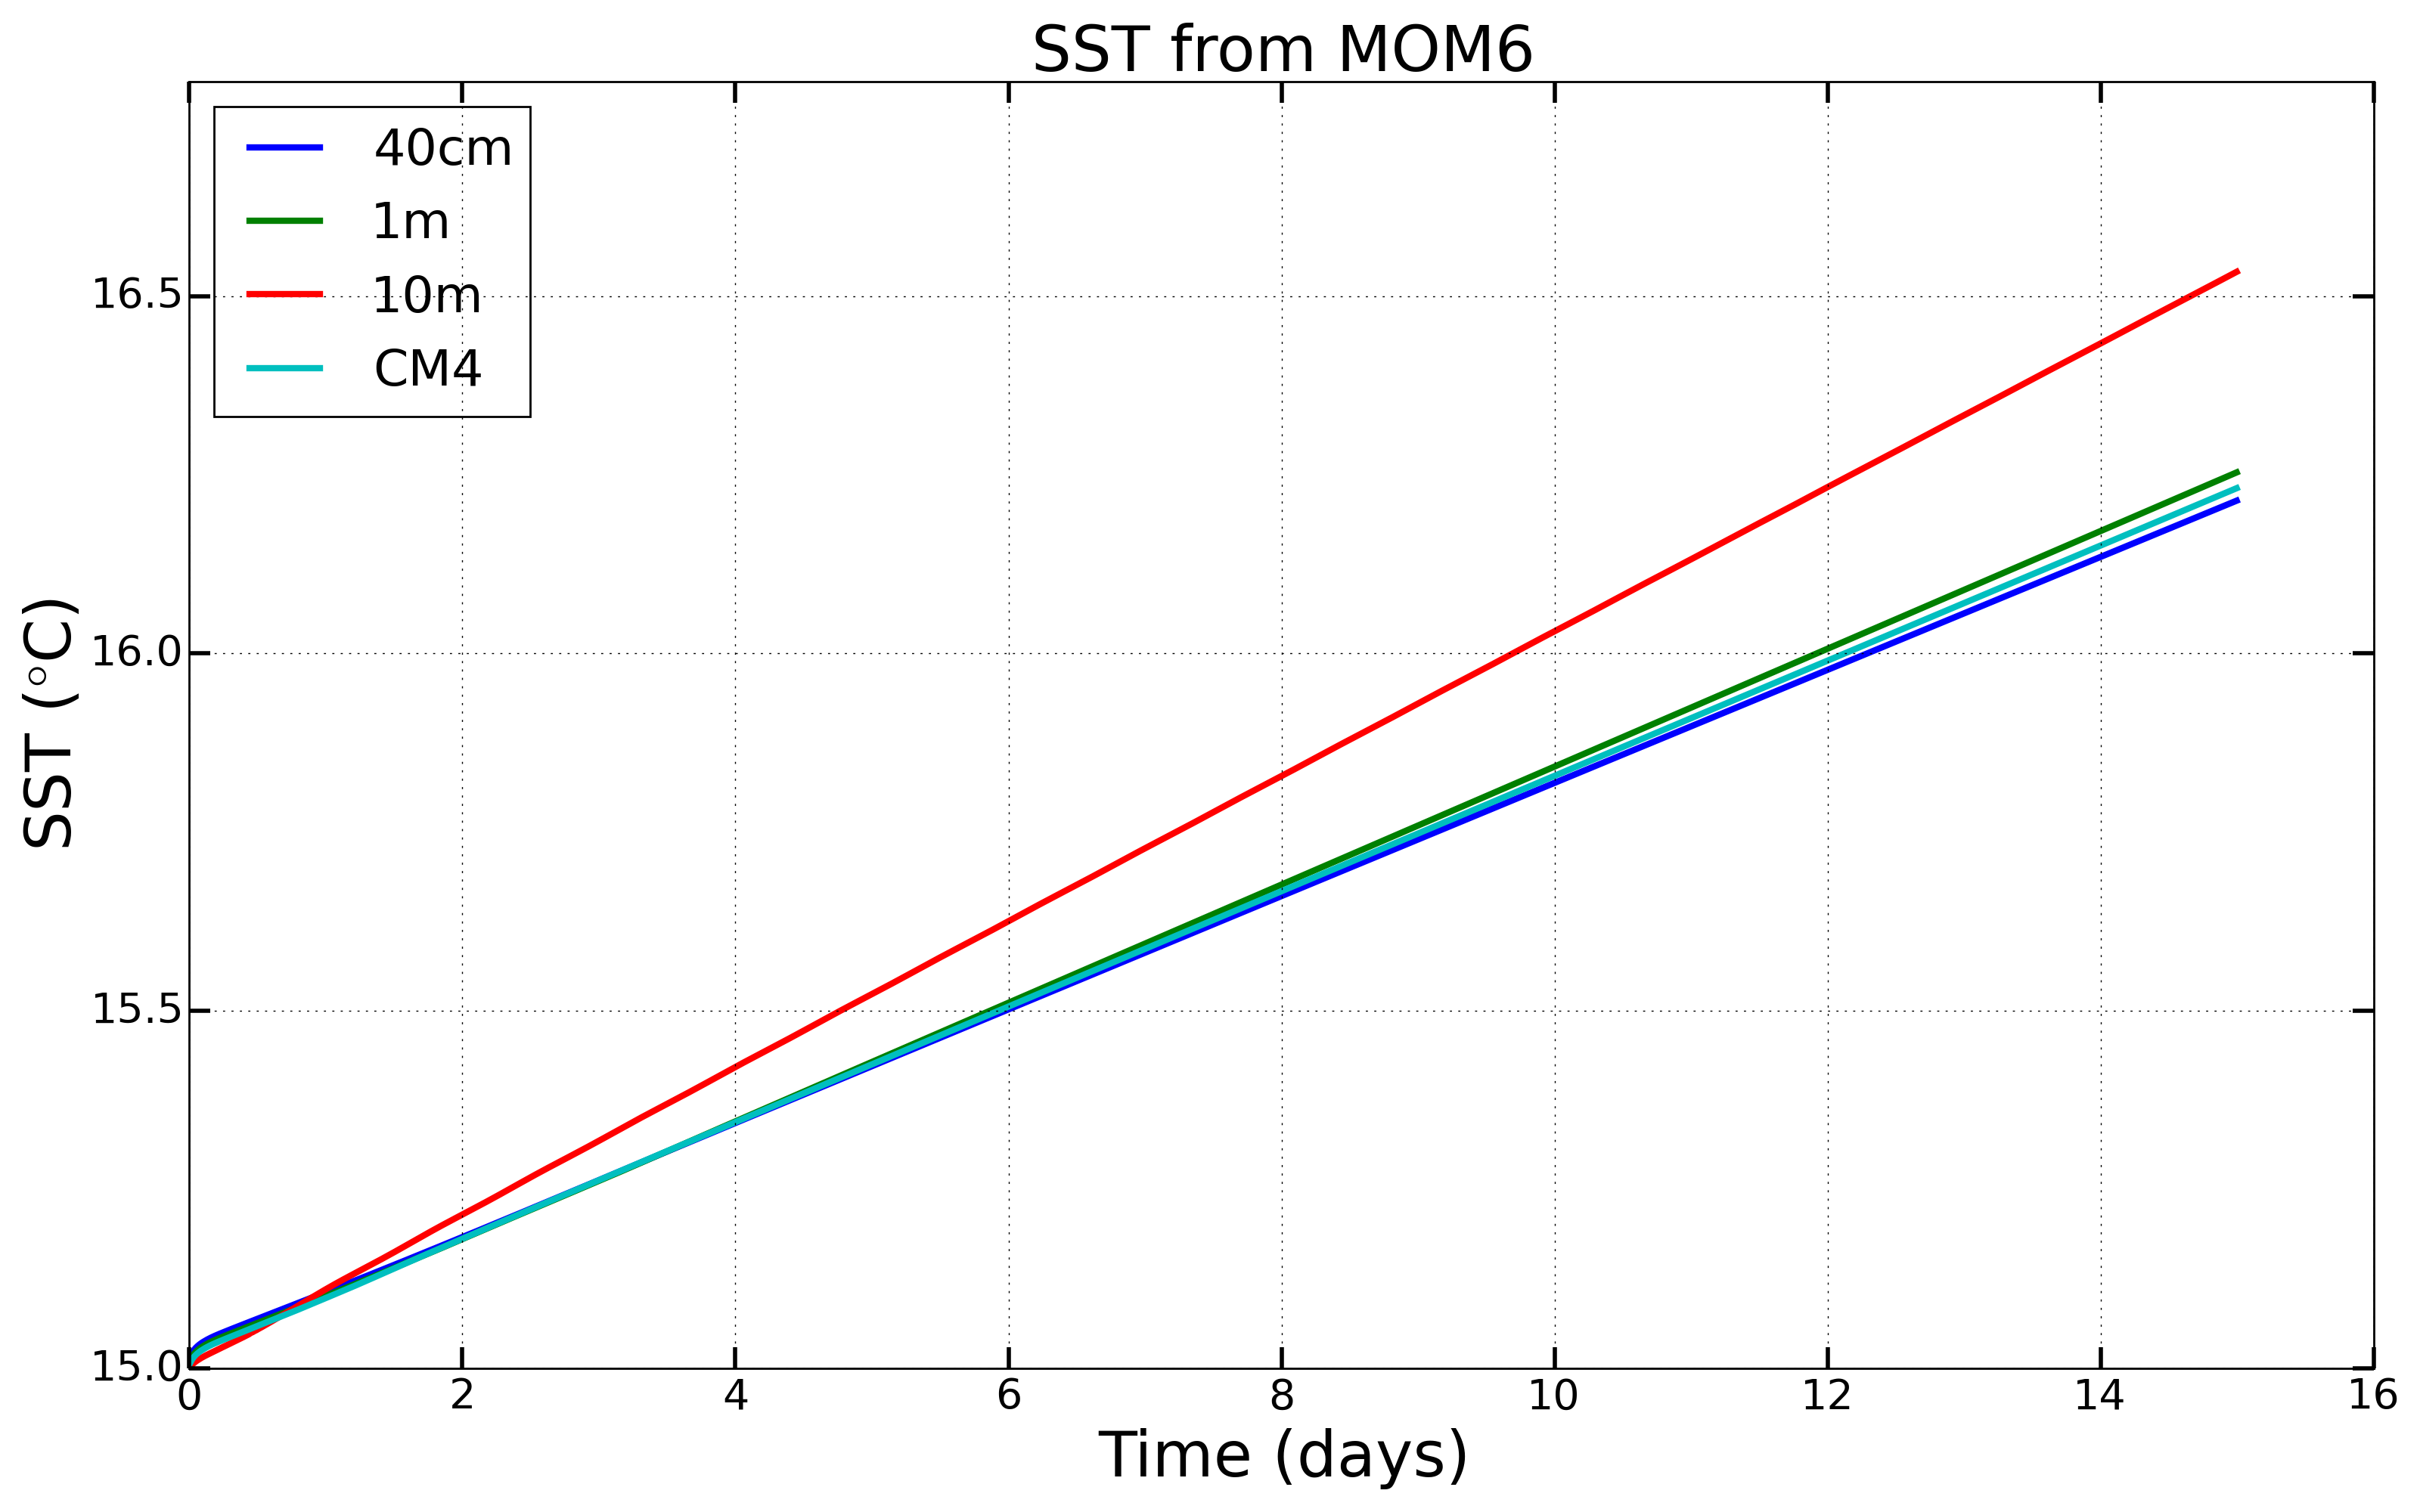
\includegraphics[angle=0,width=5cm]{./figs/MOM6/skin_warming_wind_KPP_MOM6_SST.png}
\caption[KPP BL depth, ML depth, and SST from MOM6 for warming+winds
test]{\sf Time series for KPP boundary layer depth (left panel), mixed
  layer depth (middle panel), and SST (right panel) for the
  warming+wind test case (constant zonal wind stress and
  $Q=100~\mbox{W}~\mbox{m}^{-2}$) as realized in MOM6.  The mixed
  layer depth is diagnosed as the depth where density differs from the
  surface by $0.003~\mbox{kg}~\mbox{m}^{-3}.$}
\label{fig:MOM6_SST_bldepth-wind_and_heating}
\end{center}
%\rule{\textwidth}{0.005in}
\end{figure}
%%%%%%%%%%%%%%%%%%%%%%%%%%%%%%%%%%%%%%%%%%%%%%%%%%%%%%%%%%%%%%%%%%%%%%%%


%%%%%%%%%%%%%%%%%%%% %%%%%%%%%%%%%%%%%%%%%%%%%
\begin{figure}[h!t]
%\rule{\textwidth}{0.005in}
\begin{center}
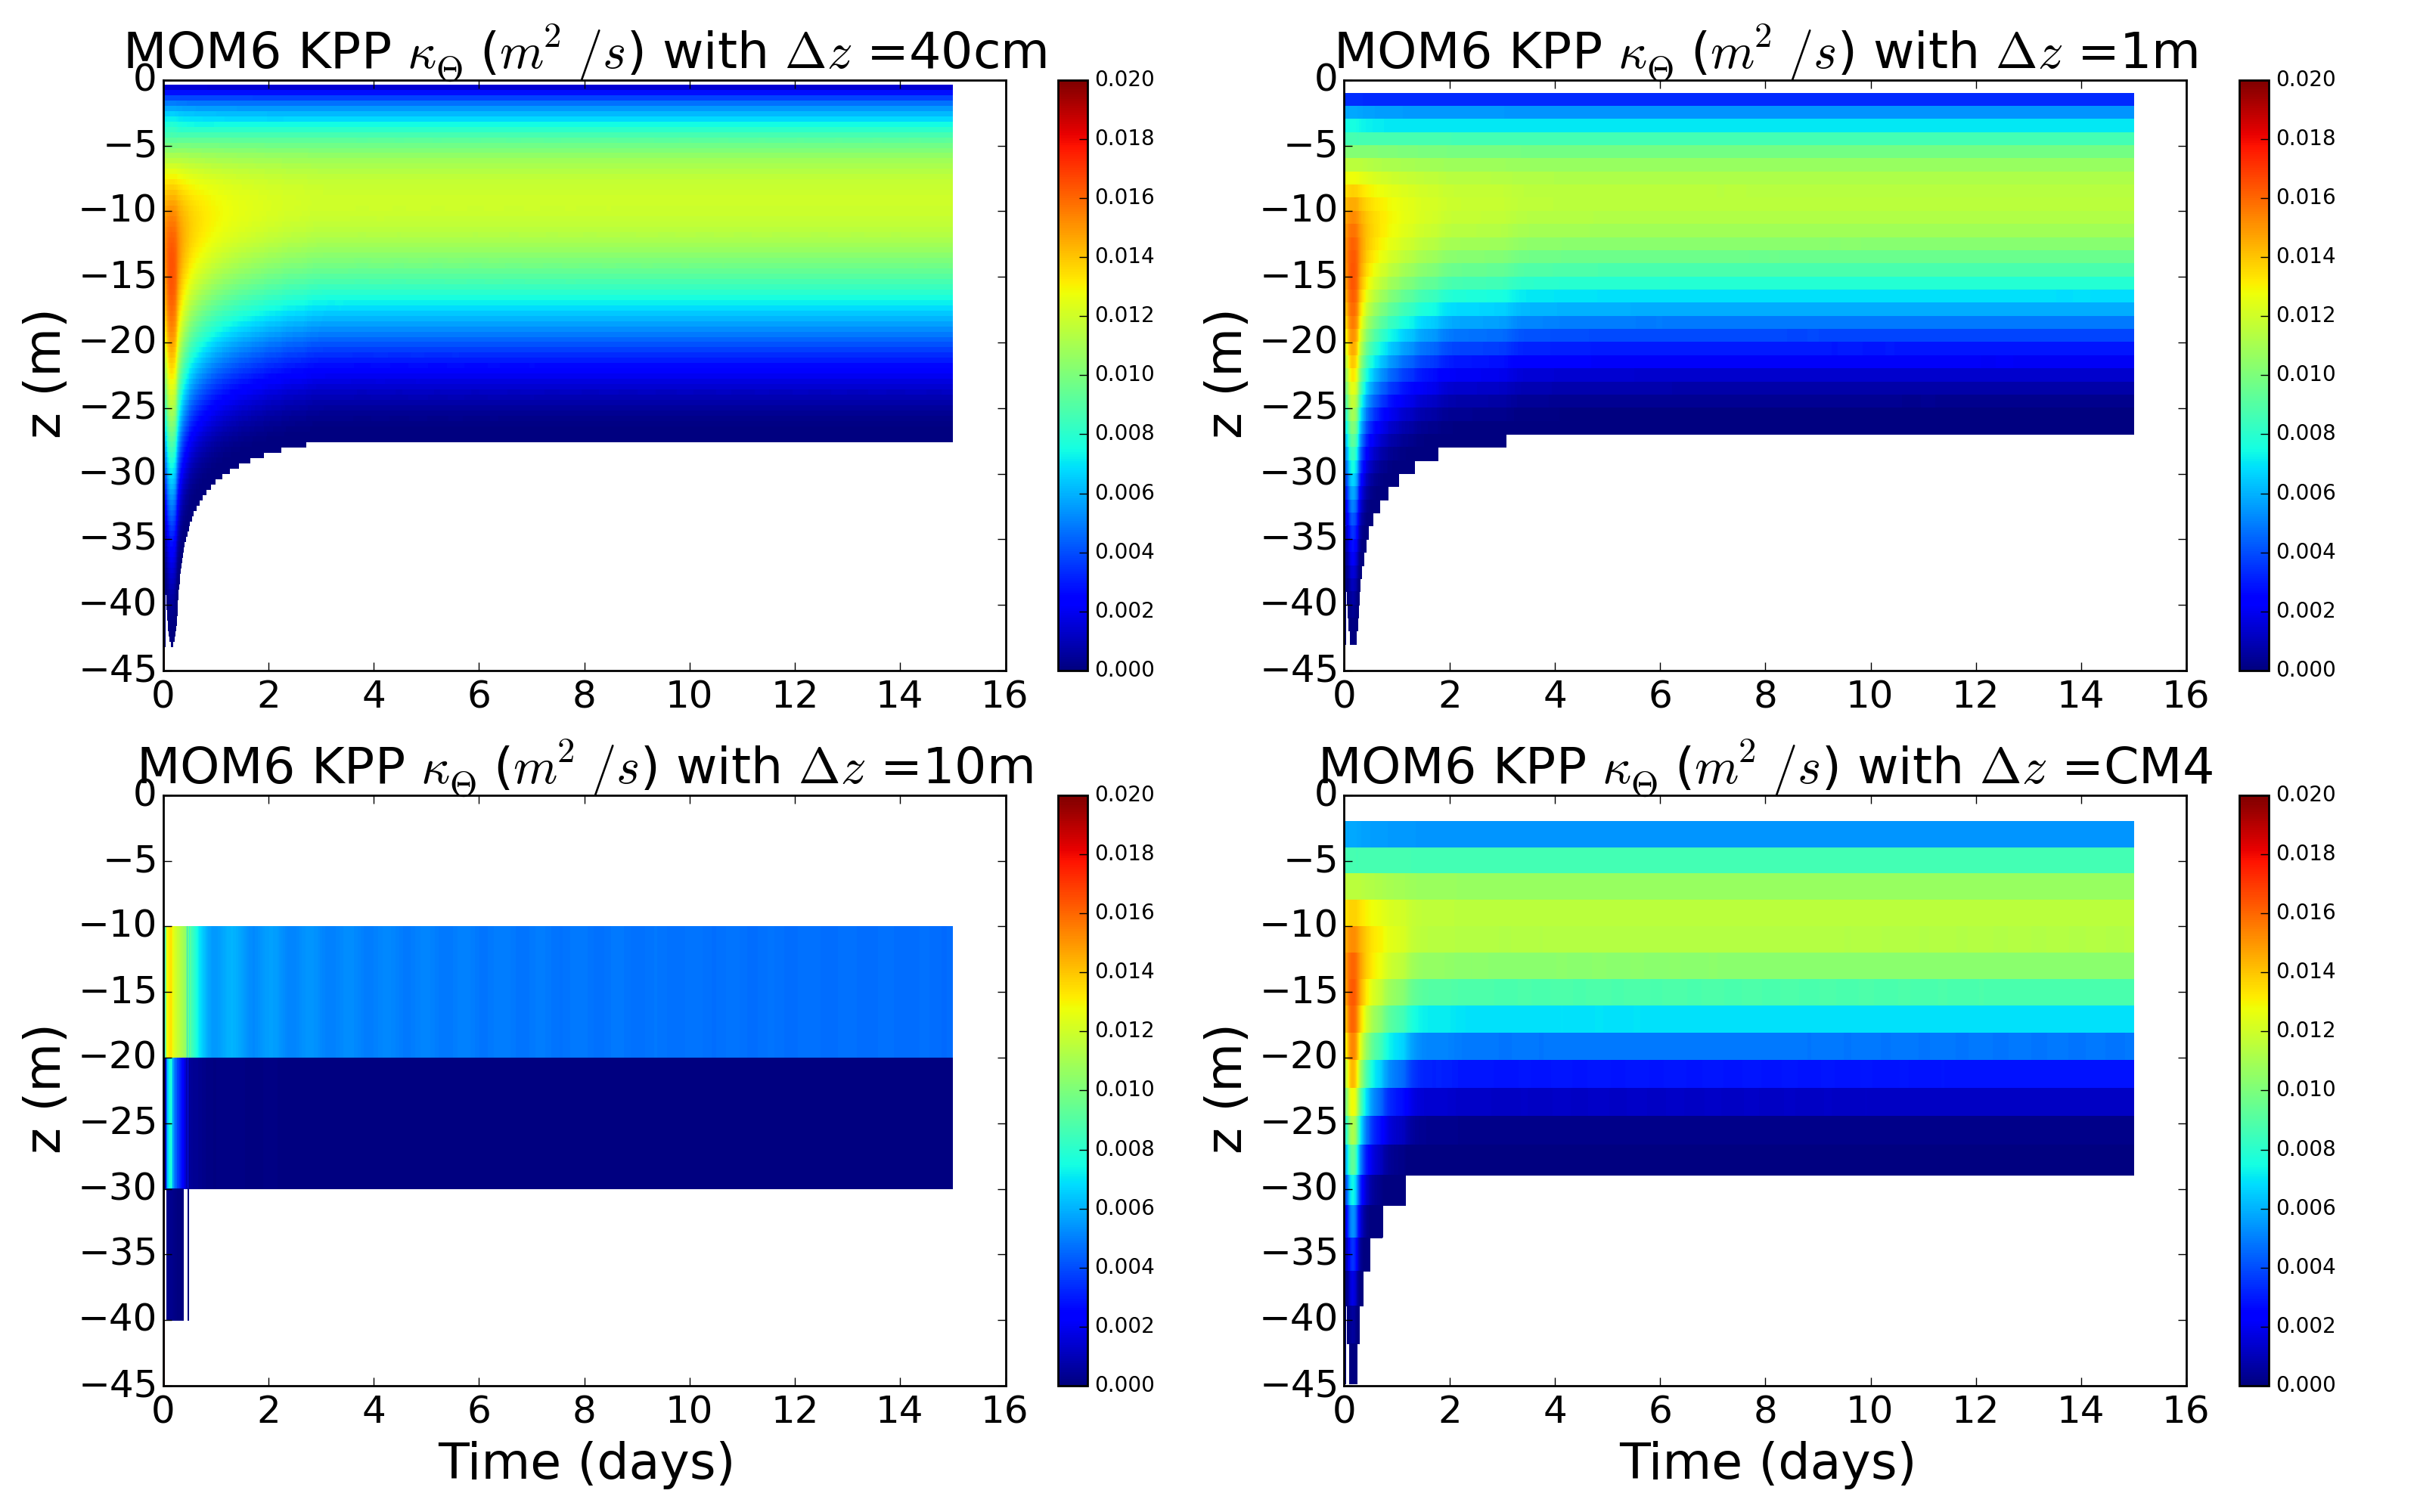
\includegraphics[angle=0,width=14cm]{./figs/MOM6/skin_warming_wind_KPP_MOM6_KPP_diffusivity.png}
\caption[KPP diffusivity from MOM6 for wind and heating test]{\sf Time
  series for the KPP vertical diffusivity for wind and heating test
  case (constant zonal wind stress and $Q=100~\mbox{W}~\mbox{m}^{-2}$)
  as realized in MOM6 using four different vertical grid resolutions.}
\label{fig:MOM6_KPP_diffusivity-wind_and_heating}
\end{center}
%\rule{\textwidth}{0.005in}
\end{figure}
%%%%%%%%%%%%%%%%%%%%%%%%%%%%%%%%%%%%%%%%%%%%%%%%%%%%%%%%%%%%%%%%%%%%%%%%


%%%%%%%%%%%%%%%%%%%% %%%%%%%%%%%%%%%%%%%%%%%%%
\begin{figure}[h!t]
%\rule{\textwidth}{0.005in}
\begin{center}
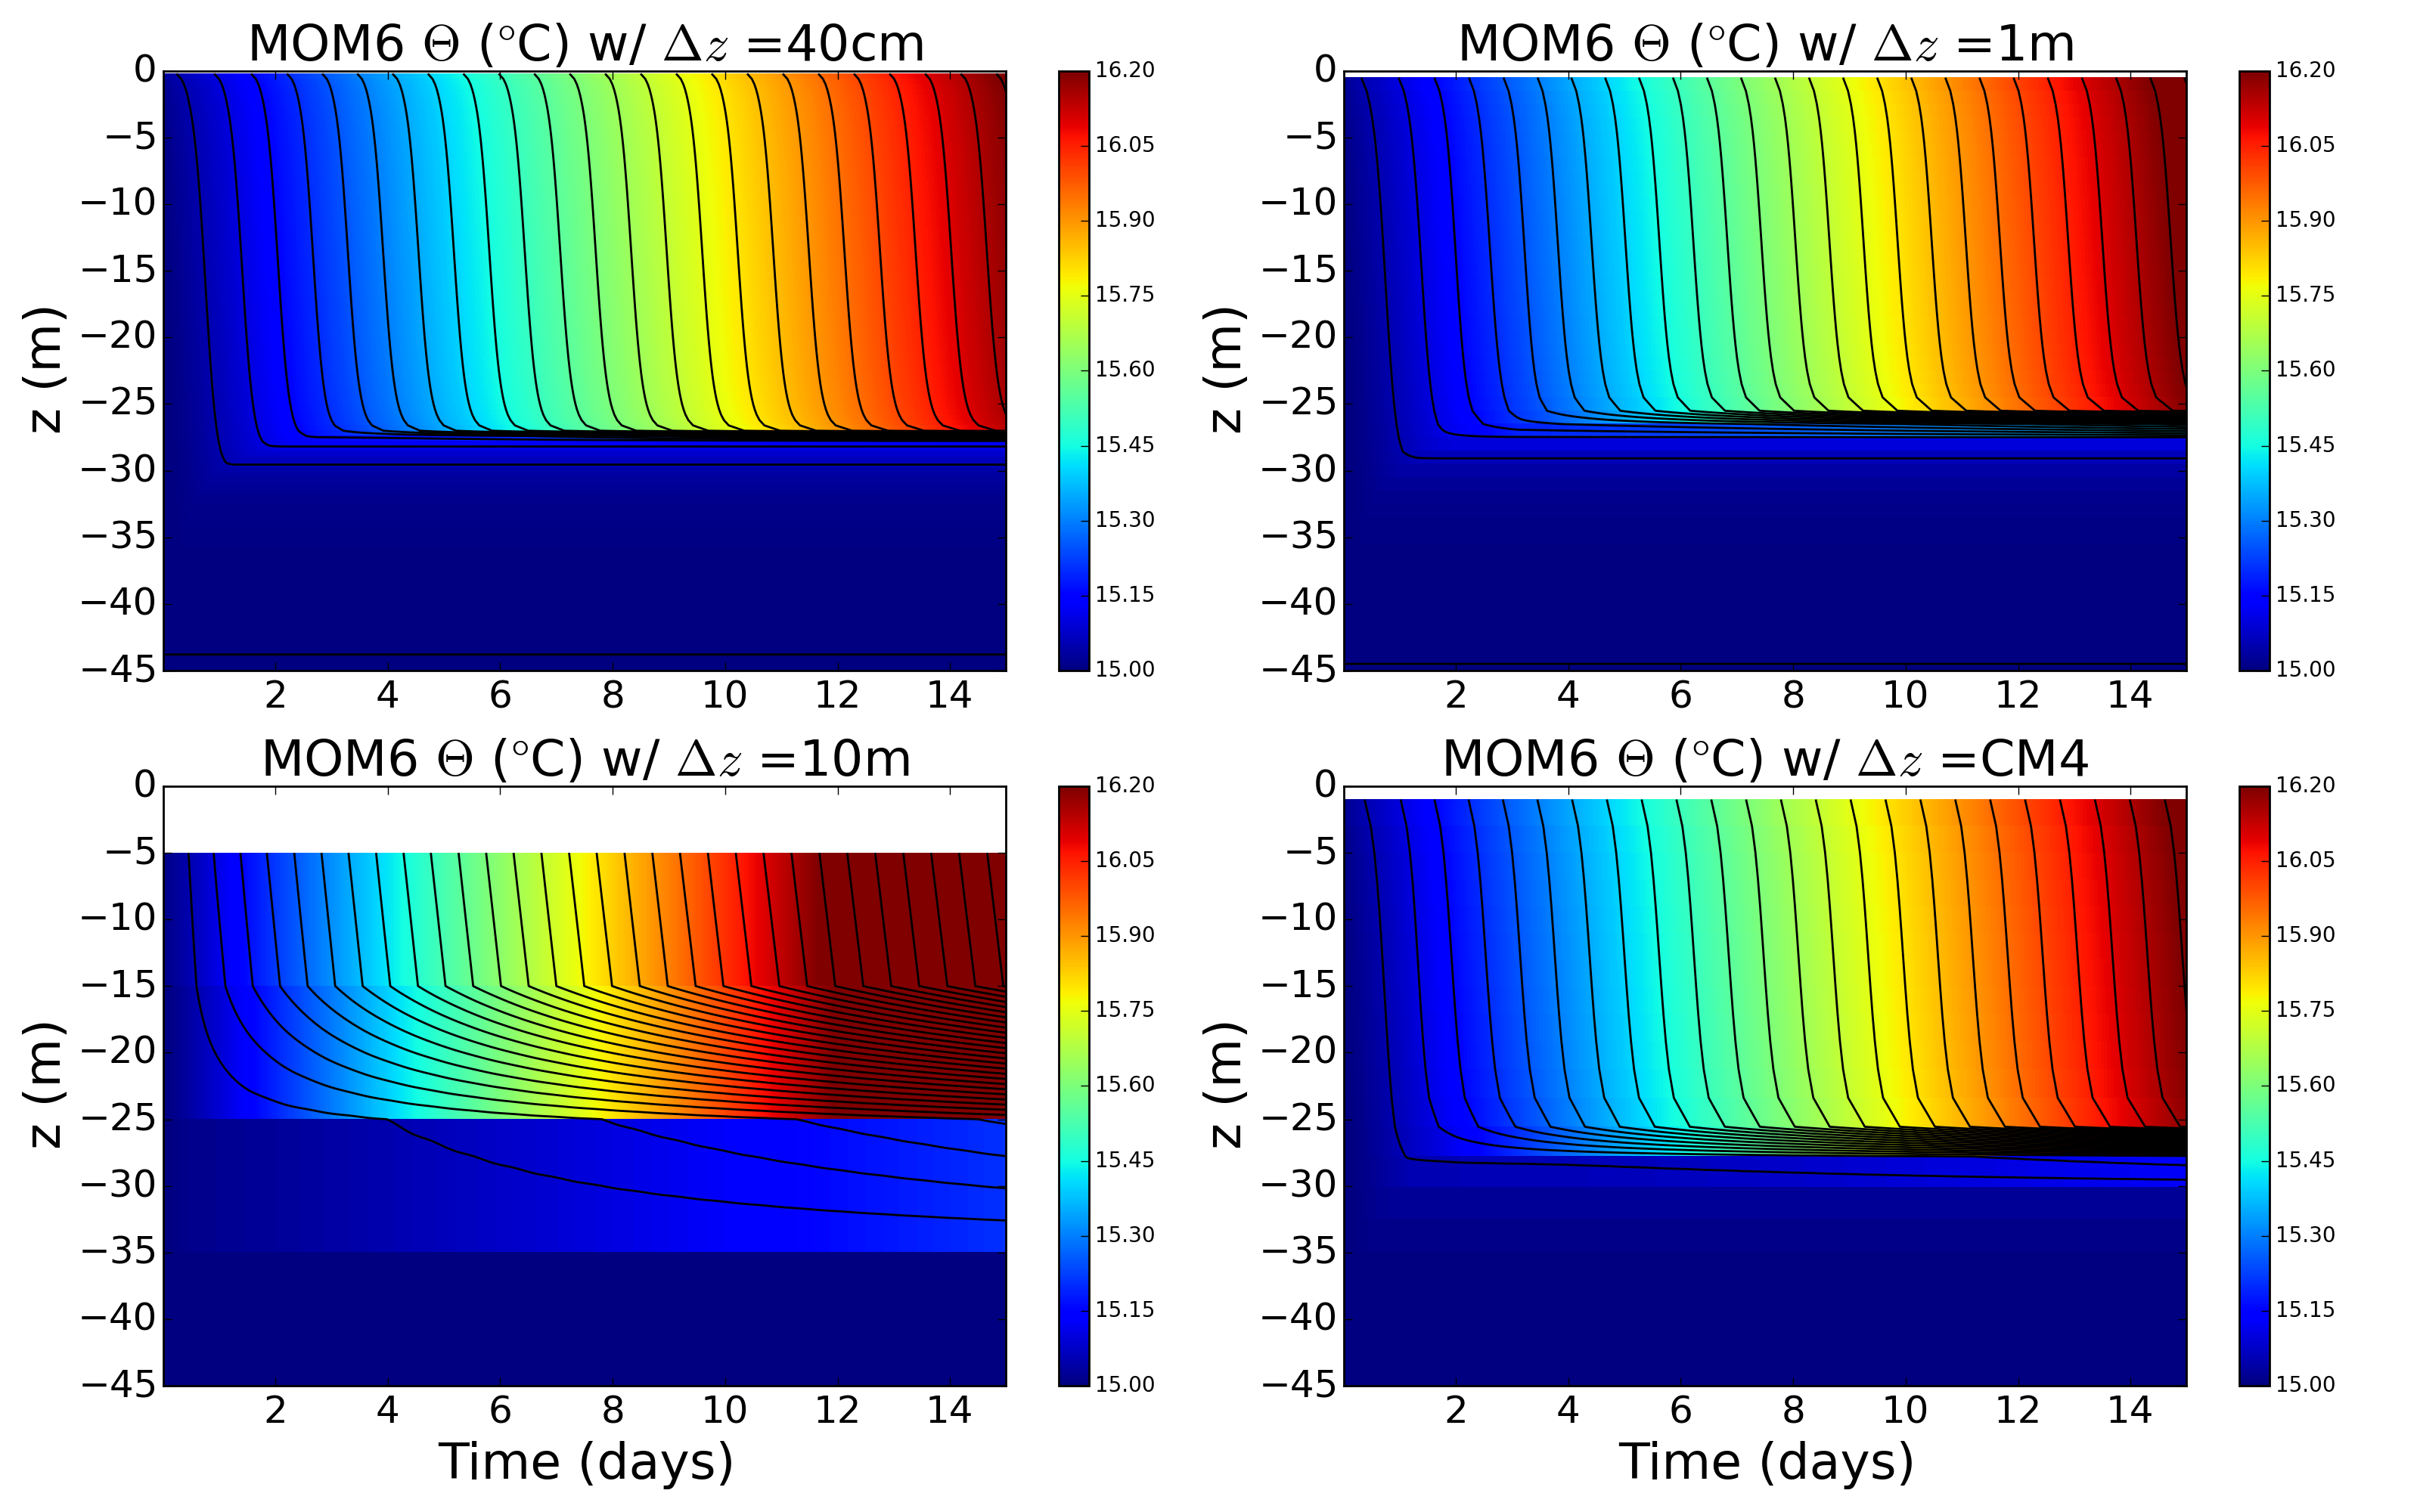
\includegraphics[angle=0,width=14cm]{./figs/MOM6/skin_warming_wind_KPP_MOM6_temp.png}
\caption[Temperature from MOM6 for wind and heating test]{\sf Time
  series for temperature from wind and heating test case (constant
  zonal wind stress and $Q=100~\mbox{W}~\mbox{m}^{-2}$) as realized in
  MOM6 using four different vertical grid resolutions.}
\label{fig:MOM6_temp-wind_and_heating}
\end{center}
%\rule{\textwidth}{0.005in}
\end{figure}
%%%%%%%%%%%%%%%%%%%%%%%%%%%%%%%%%%%%%%%%%%%%%%%%%%%%%%%%%%%%%%%%%%%%%%%%

%%%%%%%%%%%%%%%%%%%% %%%%%%%%%%%%%%%%%%%%%%%%%
\begin{figure}[h!t]
%\rule{\textwidth}{0.005in}
\begin{center}
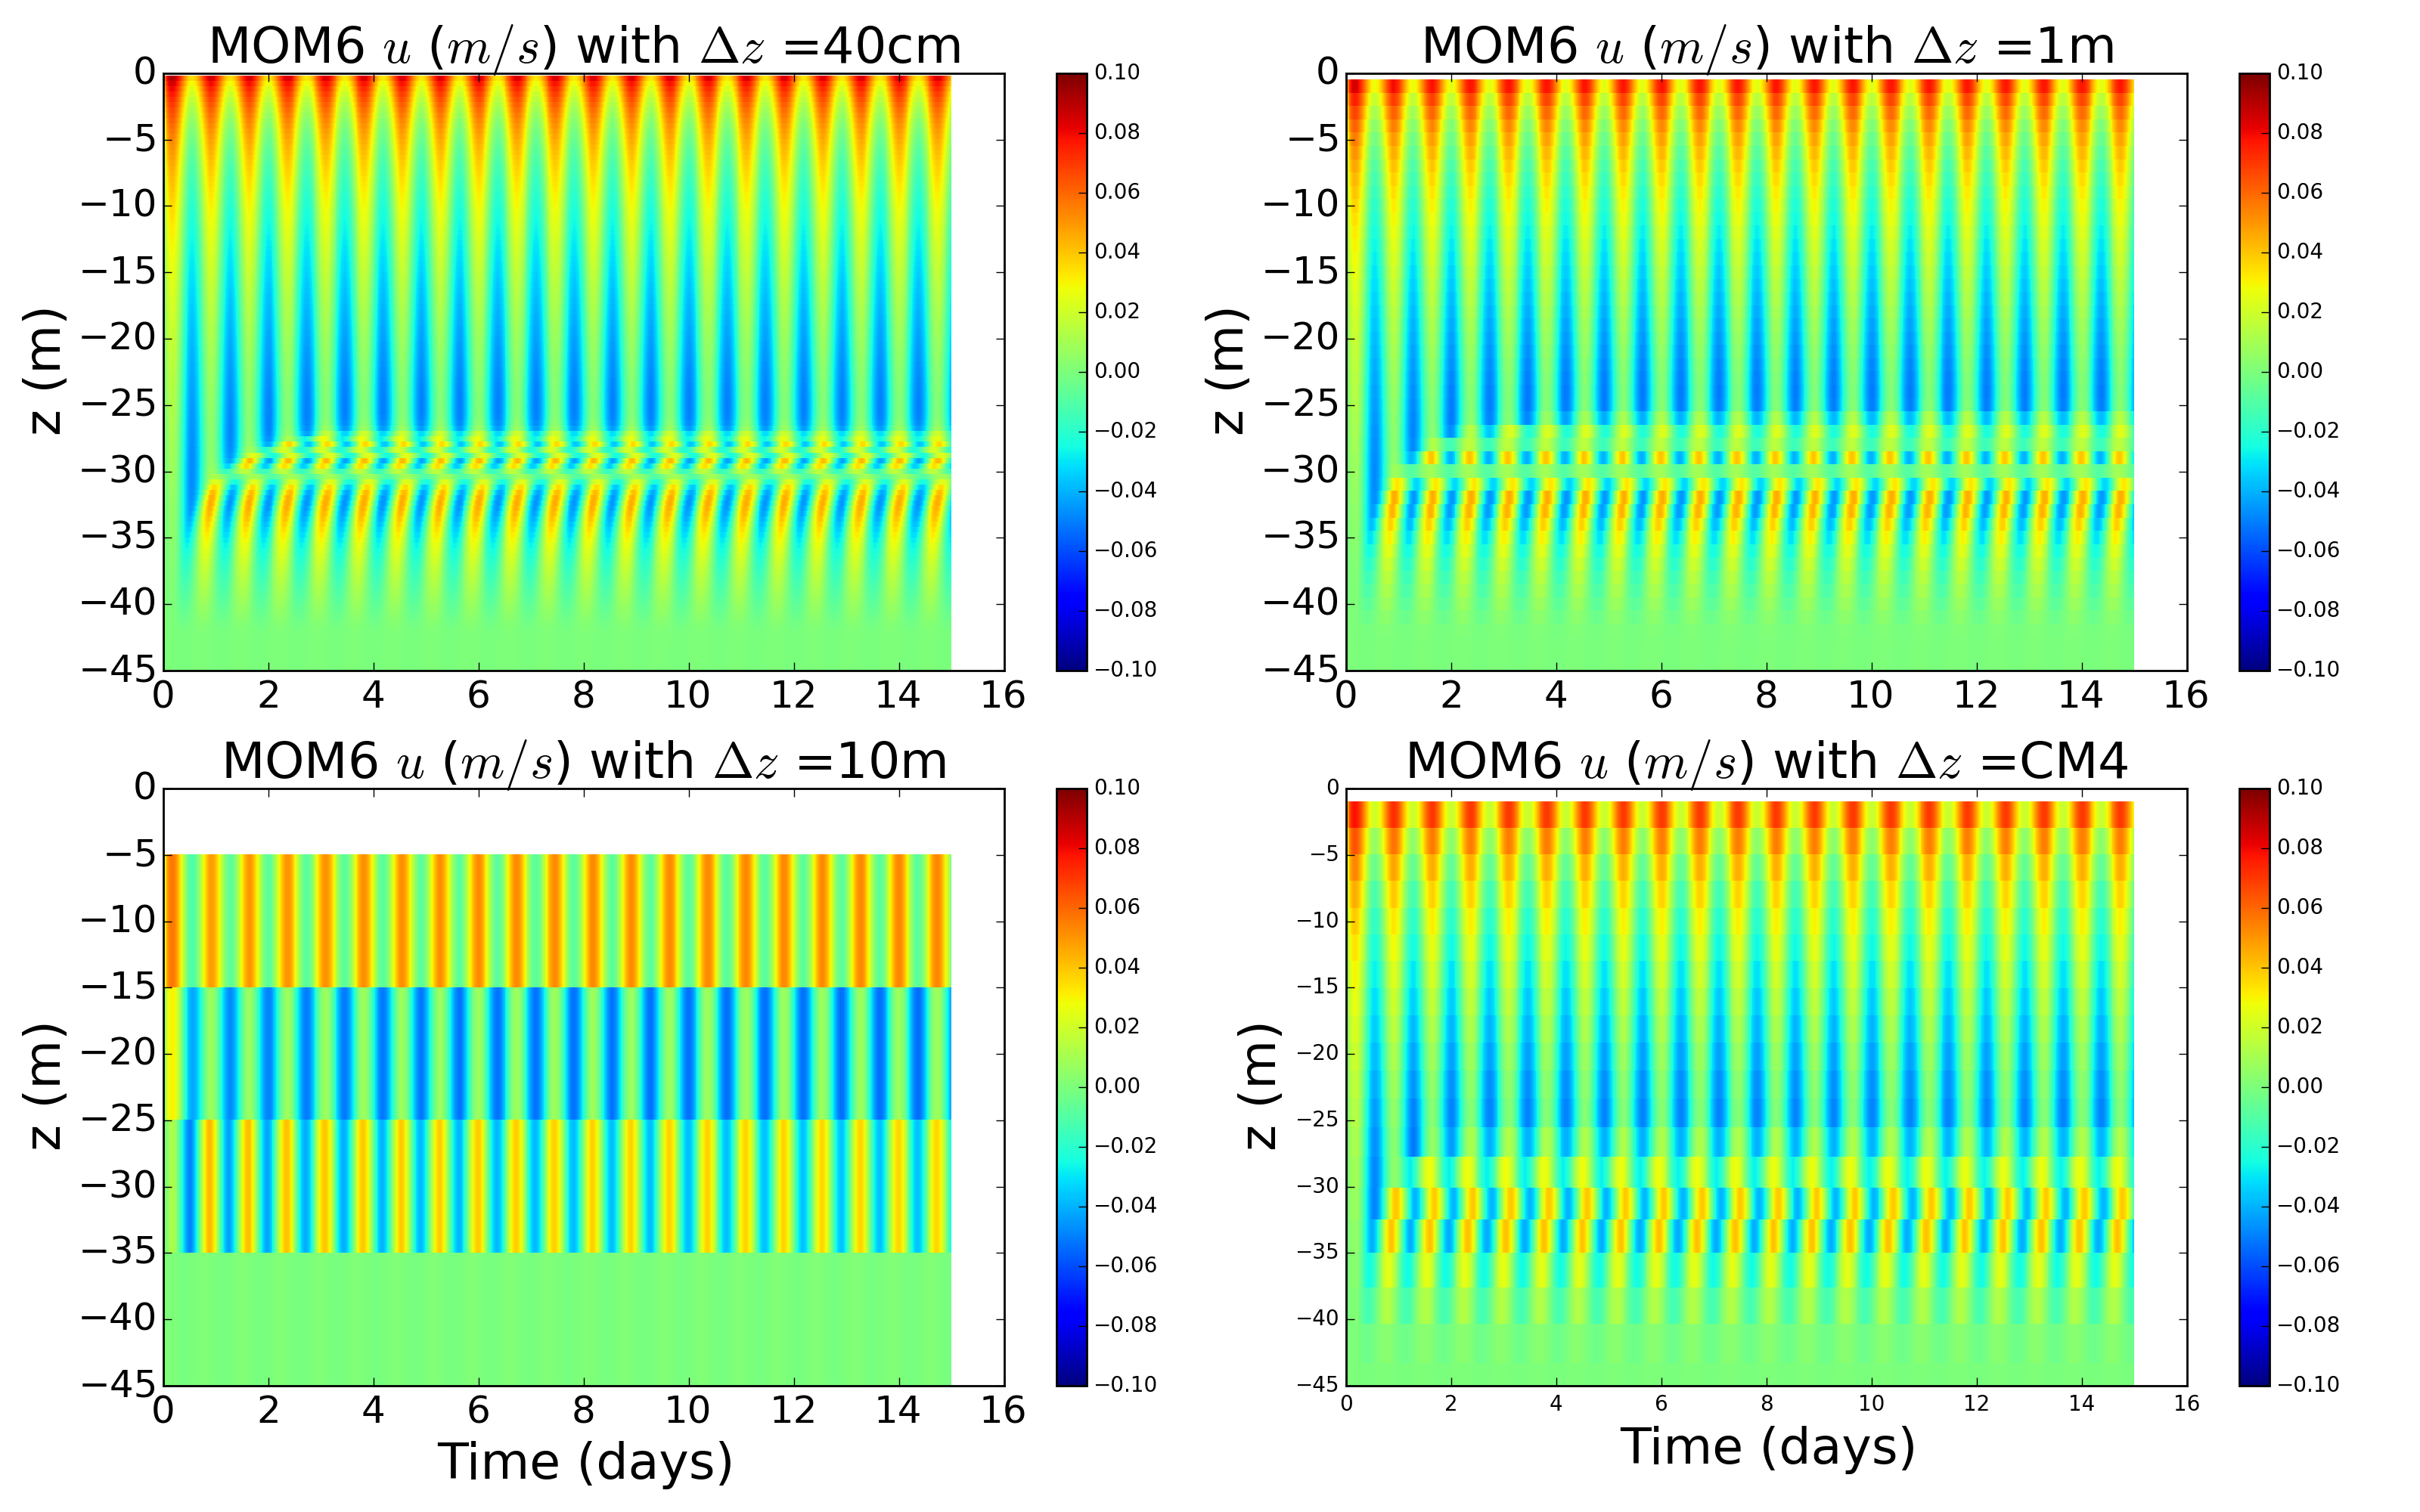
\includegraphics[angle=0,width=14cm]{./figs/MOM6/skin_warming_wind_KPP_MOM6_zonal_velocity.png}
\caption[Zonal velocity from MOM6 for wind and heating test]{\sf Time
  series for zonal velocity from wind and heating test case (constant
  zonal wind stress and $Q=100~\mbox{W}~\mbox{m}^{-2}$) as realized in
  MOM6 using four different vertical grid resolutions.}
\label{fig:MOM6_zonal-wind_and_heating}
\end{center}
%\rule{\textwidth}{0.005in}
\end{figure}
%%%%%%%%%%%%%%%%%%%%%%%%%%%%%%%%%%%%%%%%%%%%%%%%%%%%%%%%%%%%%%%%%%%%%%%%



\chapter{Cooling}
\label{chapter:cooling-only}

In this chapter, we document a test case configured with a zero wind
stress and constant negative heat flux
\begin{equation}
Q=-100~\mbox{W}~\mbox{m}^{-2}.
\end{equation}
Temperature is initialized with a stable linear stratification
according to equation (\ref{eq:linear-stratification}).  Cooling acts
to deepen the boundary layer and thus to eat away at the linear
stratification. Given the zero wind stress forcing, and zero lateral
gradients, the velocity remains unchanged from its initial zero value.
This test exercises the local downgradient diffusive portion of KPP as
well as the non-local KPP transport.


\section{Results from GFDL-MOM6}
\label{section:winds_and_cooling_mom6}

Figure \ref{fig:MOM6_SST_bldepth-cooling} shows the KPP boundary layer
depth, mixed layer depth, and SST from the MOM6 implementation of
CVMix/KPP.  The boundary layer and mixed layer deepen steadily
throughout the simulation, with the SST cooling.  This behaviour is
reflected in Figure \ref{fig:MOM6_temp-cooling}, which shows the depth
profile of temperature.  Note how the four simulations track one
another rather closely, much more closely than the tests with
wind-alone (Chapter \ref{chapter:wind_alone}) or winds plus positive
surface heat flux (Chapter \ref{chapter:winds_and_heating}).

The KPP diffusivity is shown in Figure
\ref{fig:MOM6_KPP_diffusivity-cooling}, with each grid showing the
same characteristics of a steadily increasing value, with the increase
associated with the deepening boundary layer depth. Again, the four
simulations exhibit similar characteristics.  The KPP non-local
transport is shown in Figure \ref{fig:MOM6_KPP_nonlocal-cooling}.
Each grid shows the same characteristics, with a warming near the
surface and cooling towards the lower portion of the boundary layer.
This behaviour is consistent with the default profile of the non-local
contribution to KPP in the CVMix scheme.  The surface warming arises
from the redistribution of the cooling surface boundary flux
throughout the boundary layer.  That is, the non-local term warms the
top portion of the boundary layer relative to the case without the
non-local term, and cools the lower portion of the boundary layer.
  

%%%%%%%%%%%%%%%%%%%% %%%%%%%%%%%%%%%%%%%%%%%%%
\begin{figure}[h!t]
%\rule{\textwidth}{0.005in}
\begin{center}
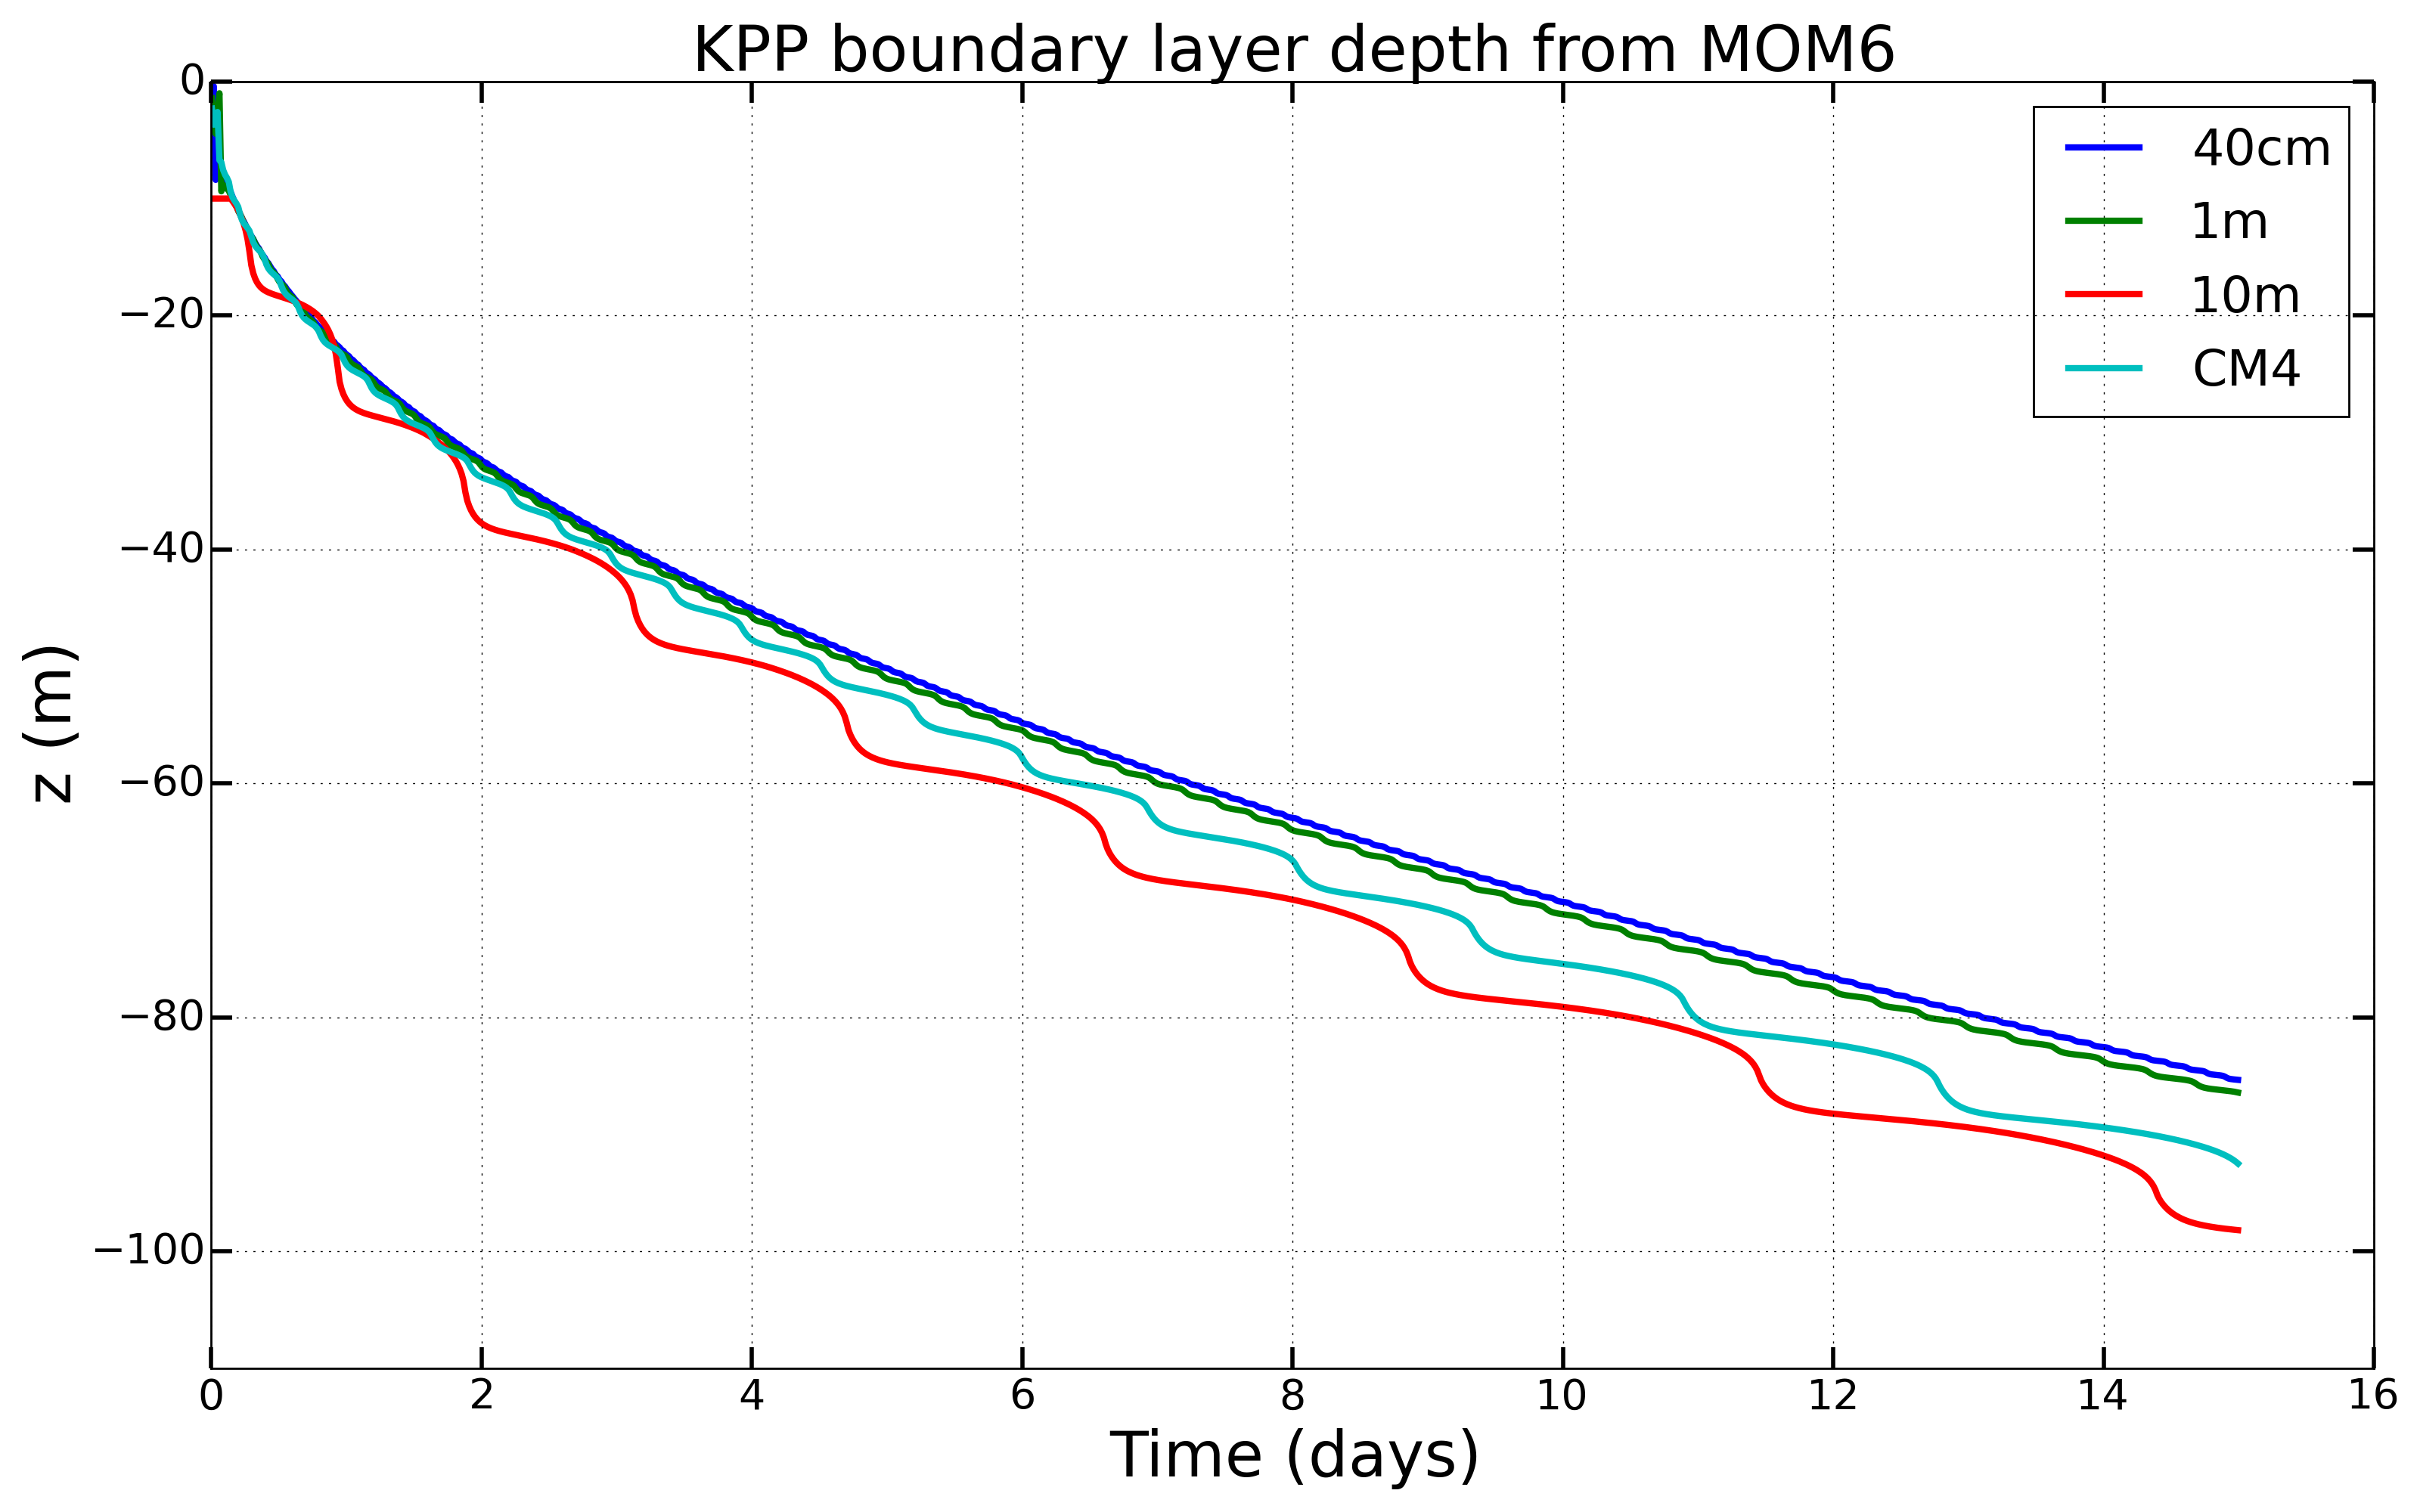
\includegraphics[angle=0,width=5cm]{./figs/MOM6/cooling_KPP_MOM6_bldepth.png}
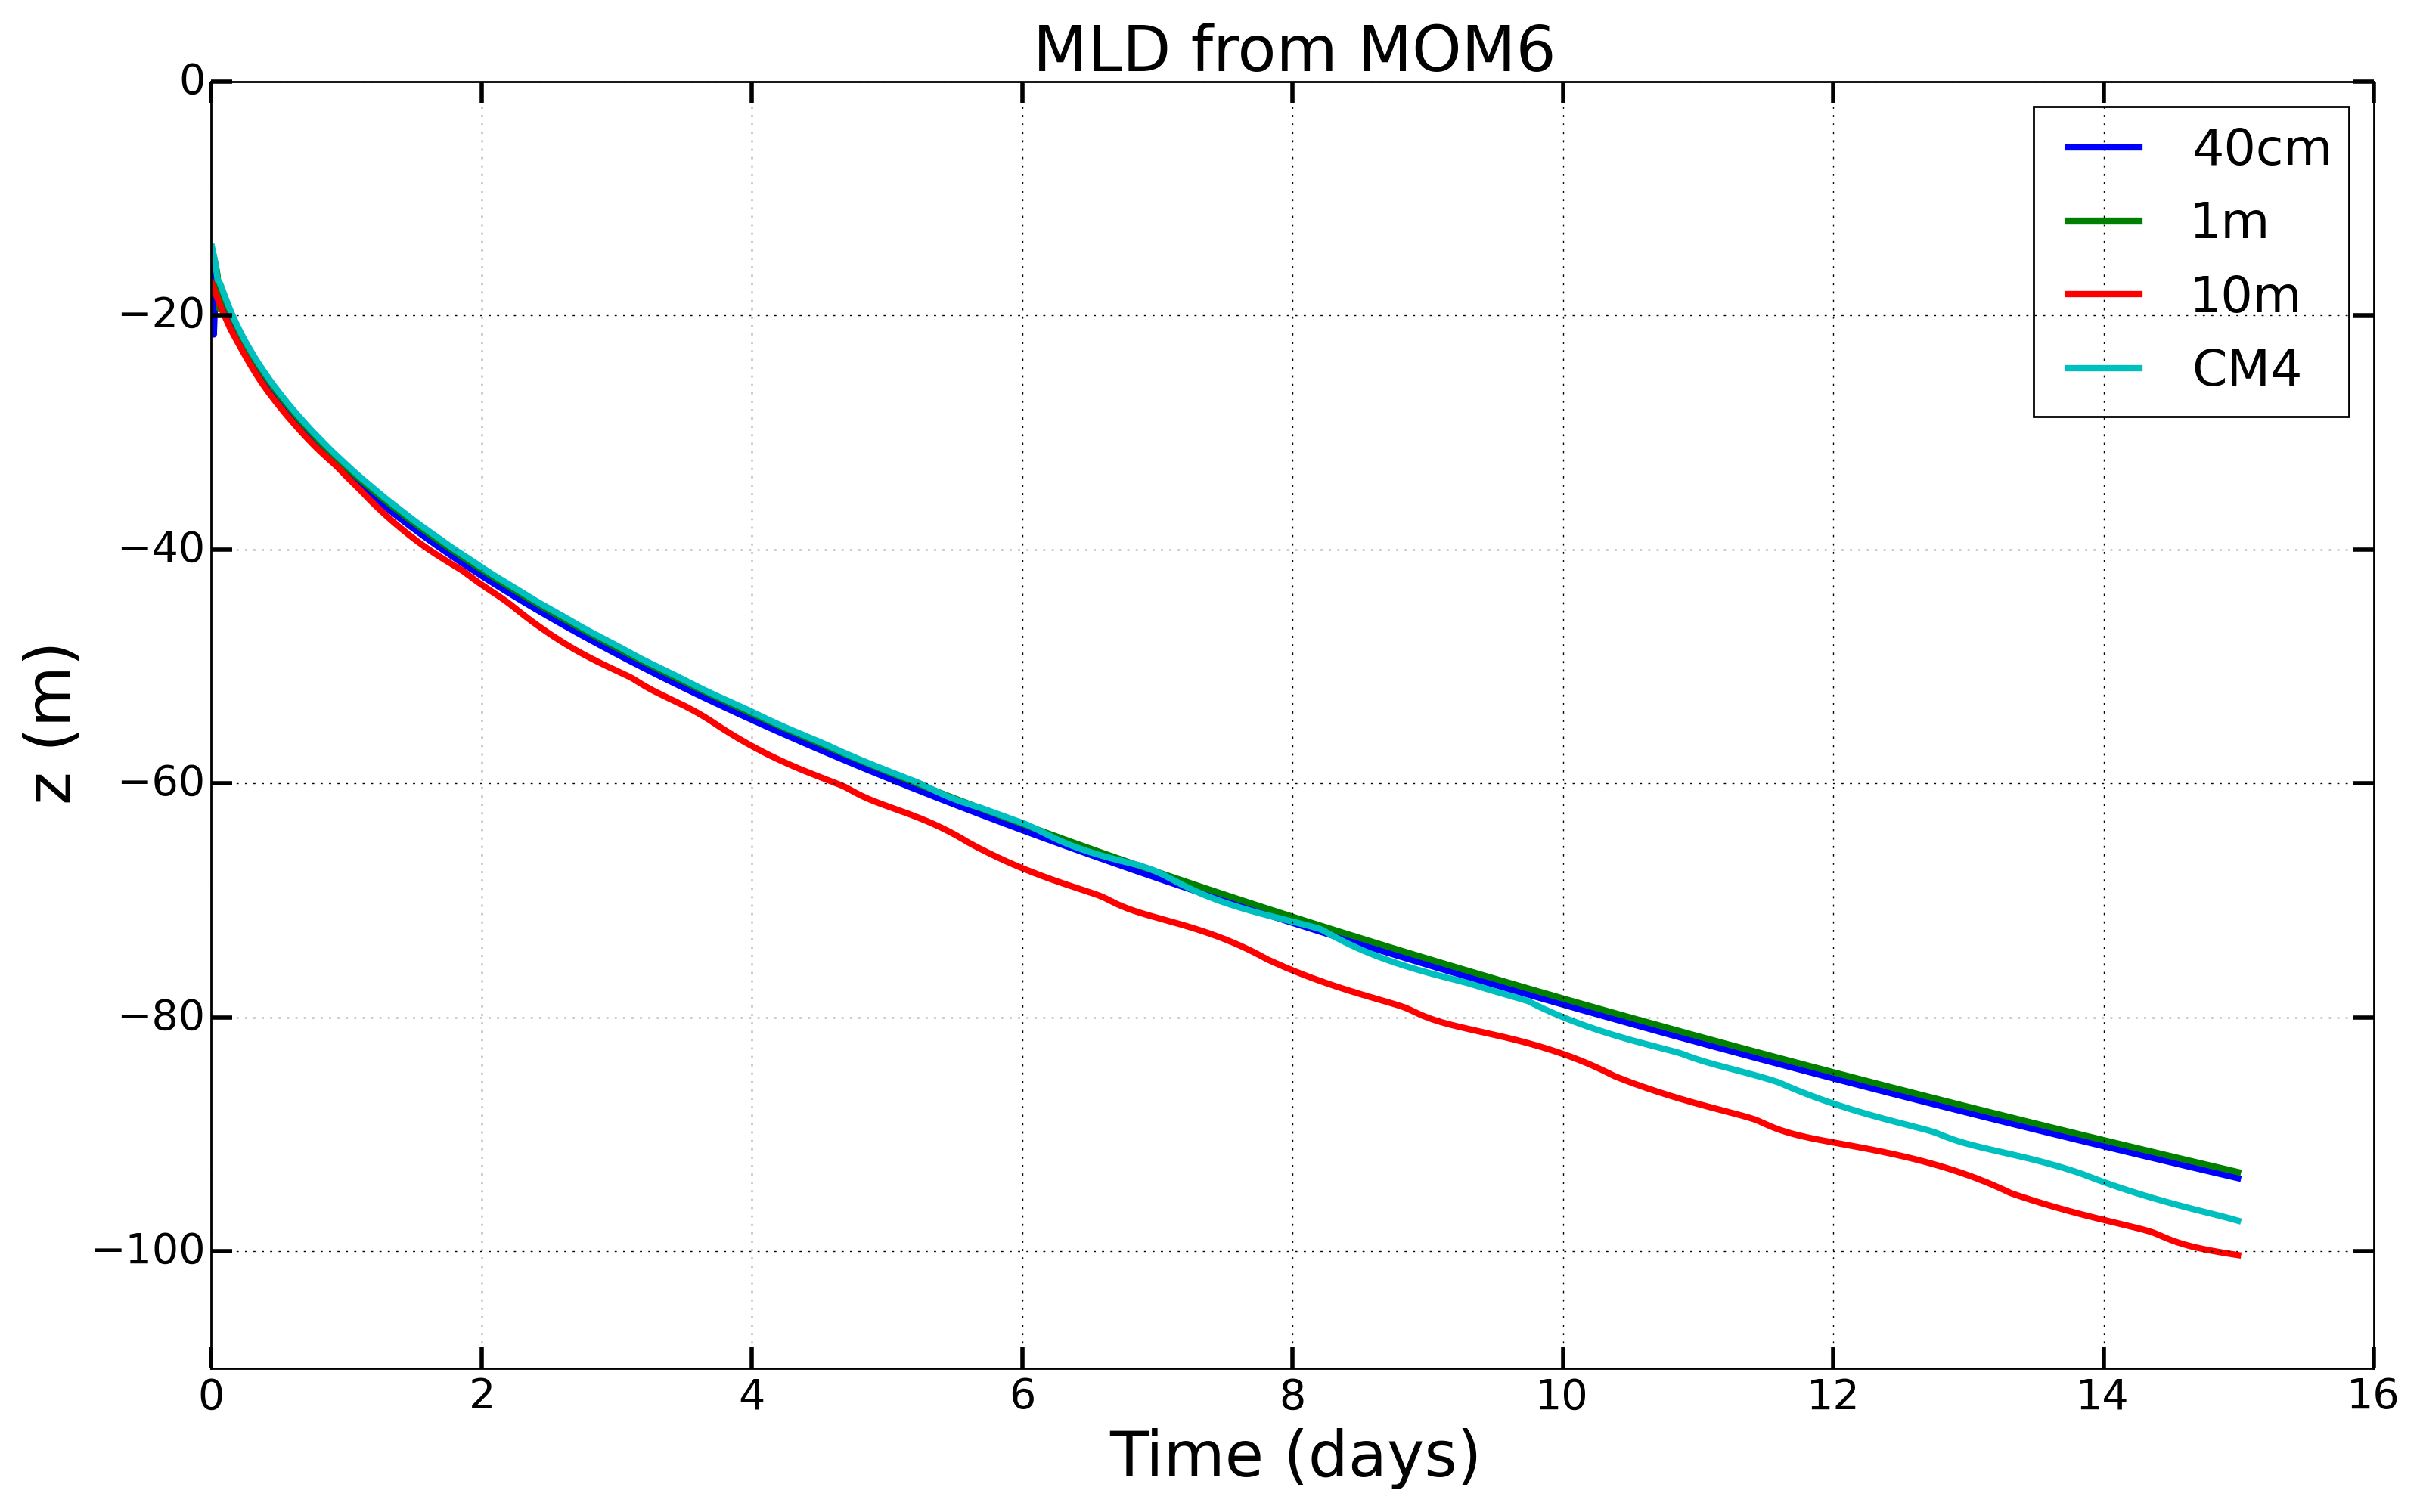
\includegraphics[angle=0,width=5cm]{./figs/MOM6/cooling_KPP_MOM6_mld.png}
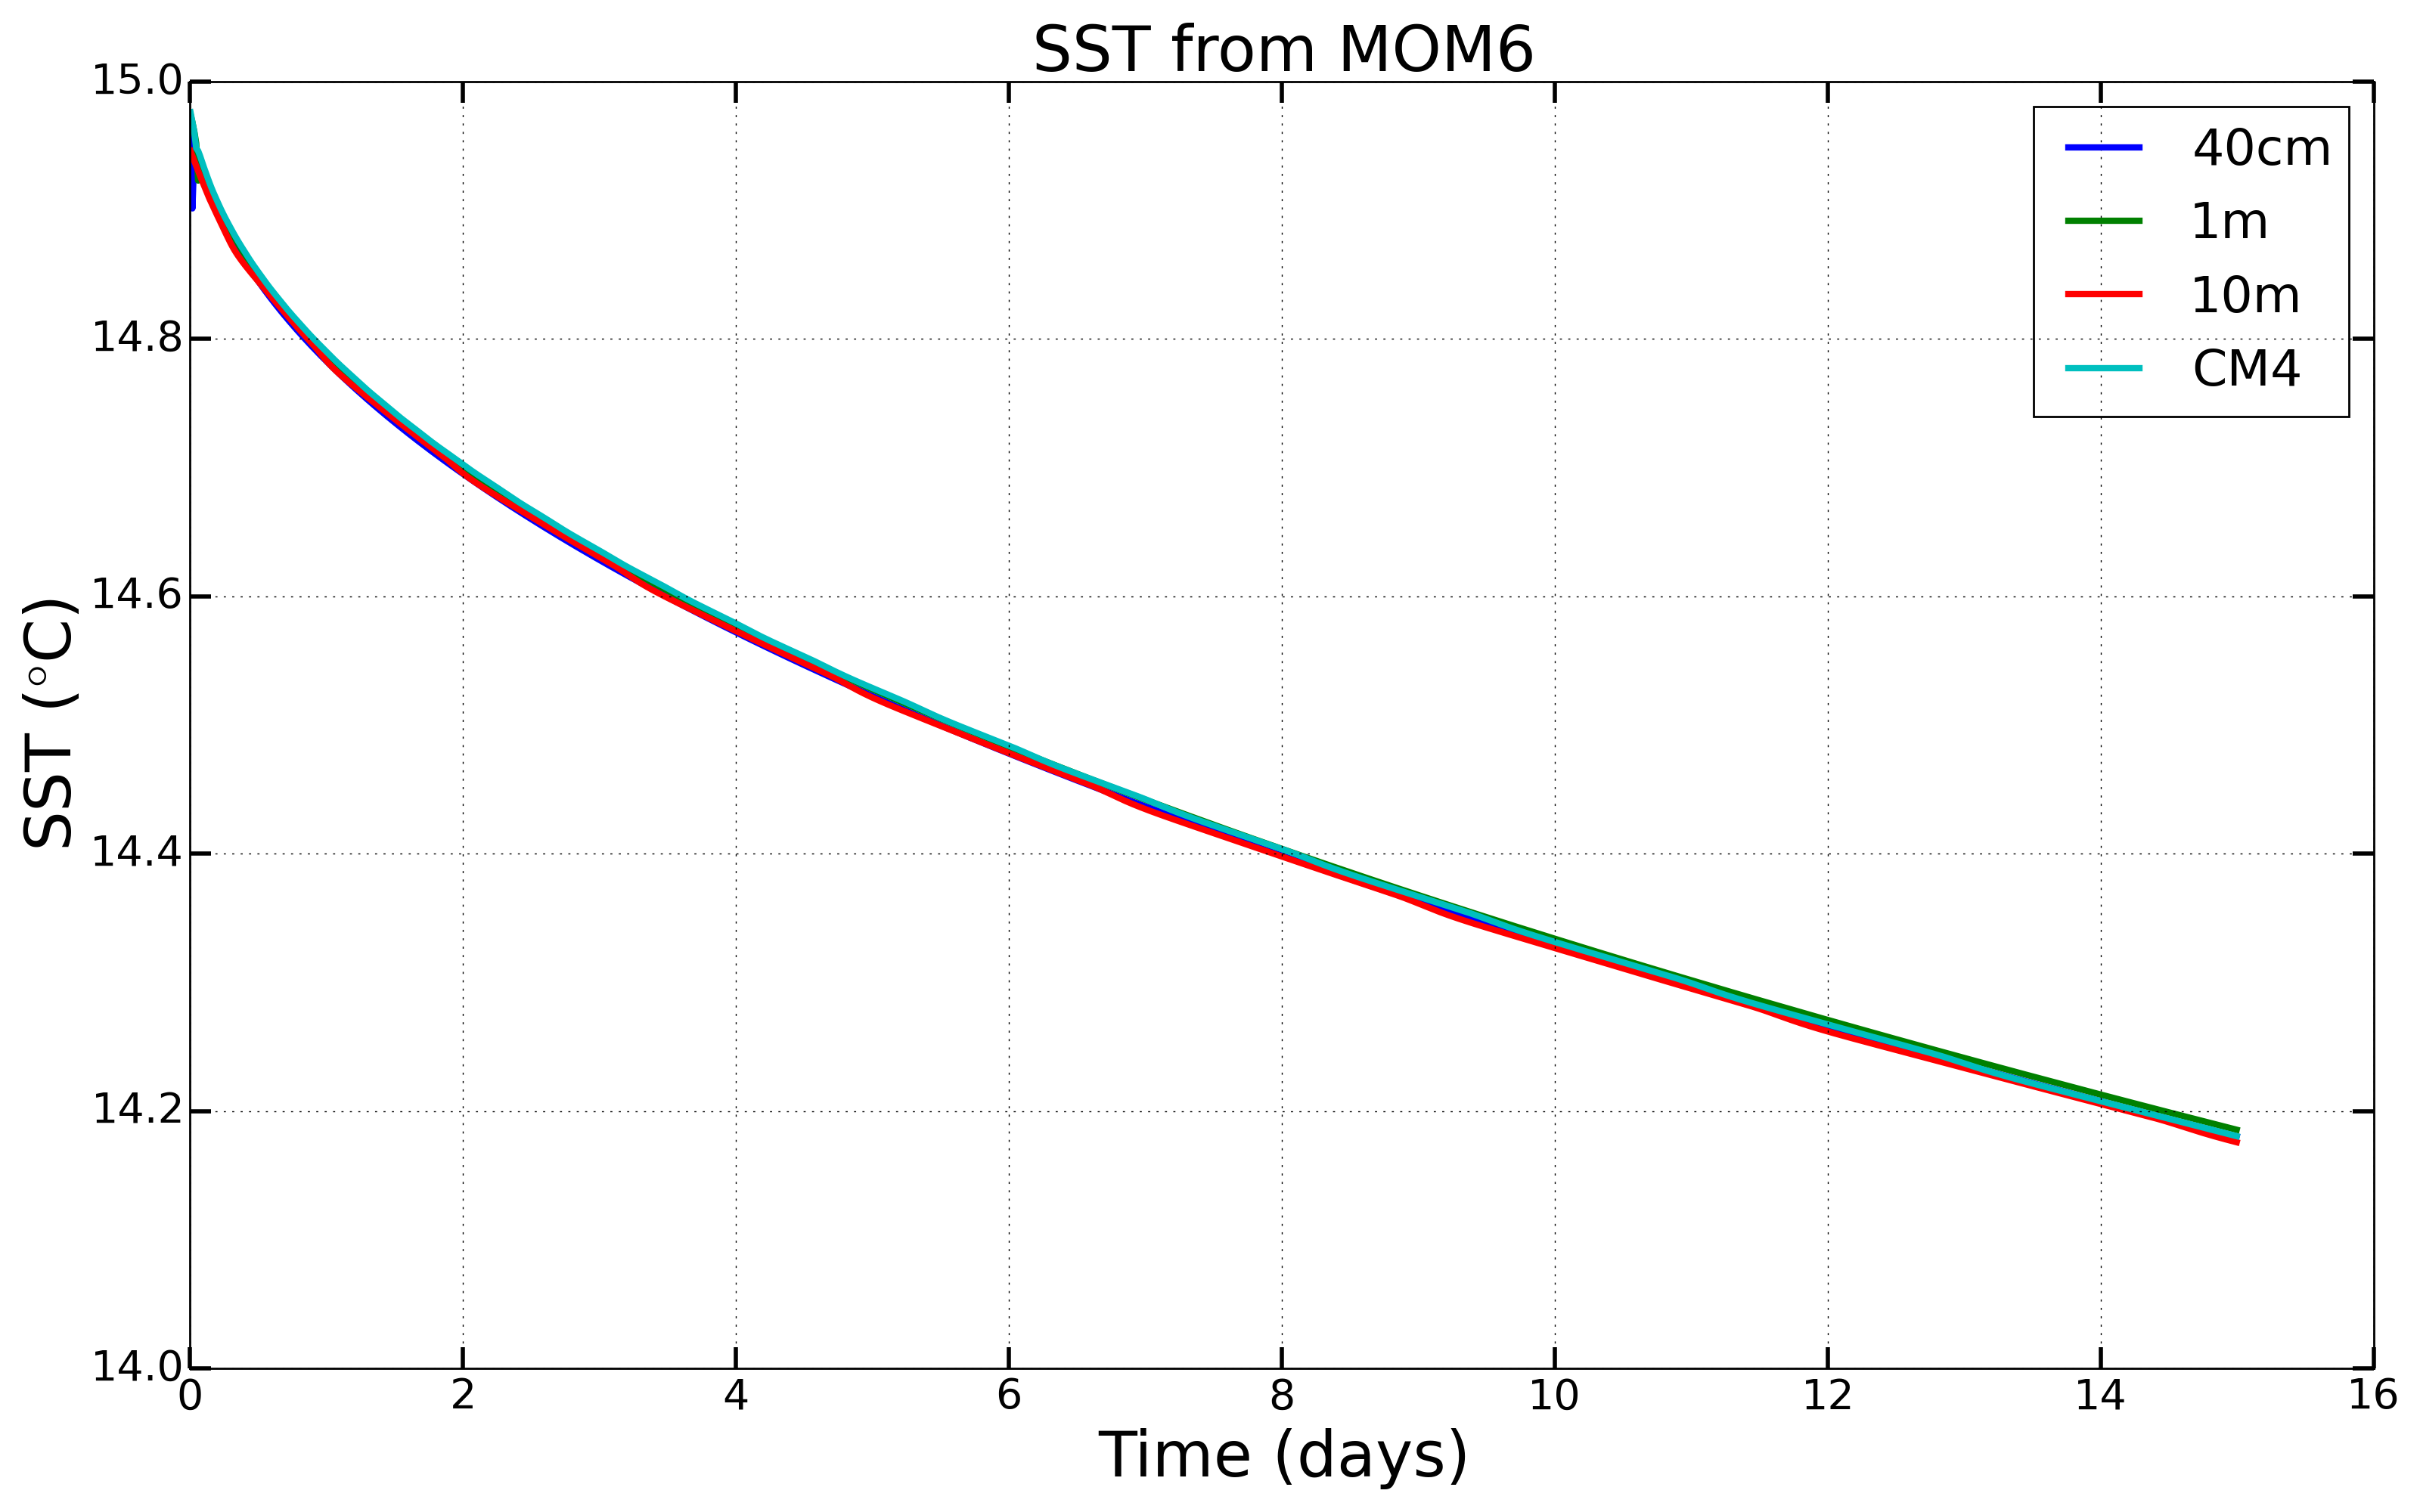
\includegraphics[angle=0,width=5cm]{./figs/MOM6/cooling_KPP_MOM6_SST.png}
\caption[KPP BL depth, ML depth, and SST from MOM6 for cooling
test]{\sf Time series for KPP boundary layer depth (left panel), mixed
  layer depth (middle panel), and SST (right panel) for the cooling
  test case (zero winds and $Q=-100~\mbox{W}~\mbox{m}^{-2}$) as
  realized in MOM6.  The mixed layer depth is diagnosed as the depth
  where density differs from the surface by
  $0.003~\mbox{kg}~\mbox{m}^{-3}.$}
\label{fig:MOM6_SST_bldepth-cooling}
\end{center}
%\rule{\textwidth}{0.005in}
\end{figure}
%%%%%%%%%%%%%%%%%%%%%%%%%%%%%%%%%%%%%%%%%%%%%%%%%%%%%%%%%%%%%%%%%%%%%%%%

%%%%%%%%%%%%%%%%%%%% %%%%%%%%%%%%%%%%%%%%%%%%%
\begin{figure}[h!t]
%\rule{\textwidth}{0.005in}
\begin{center}
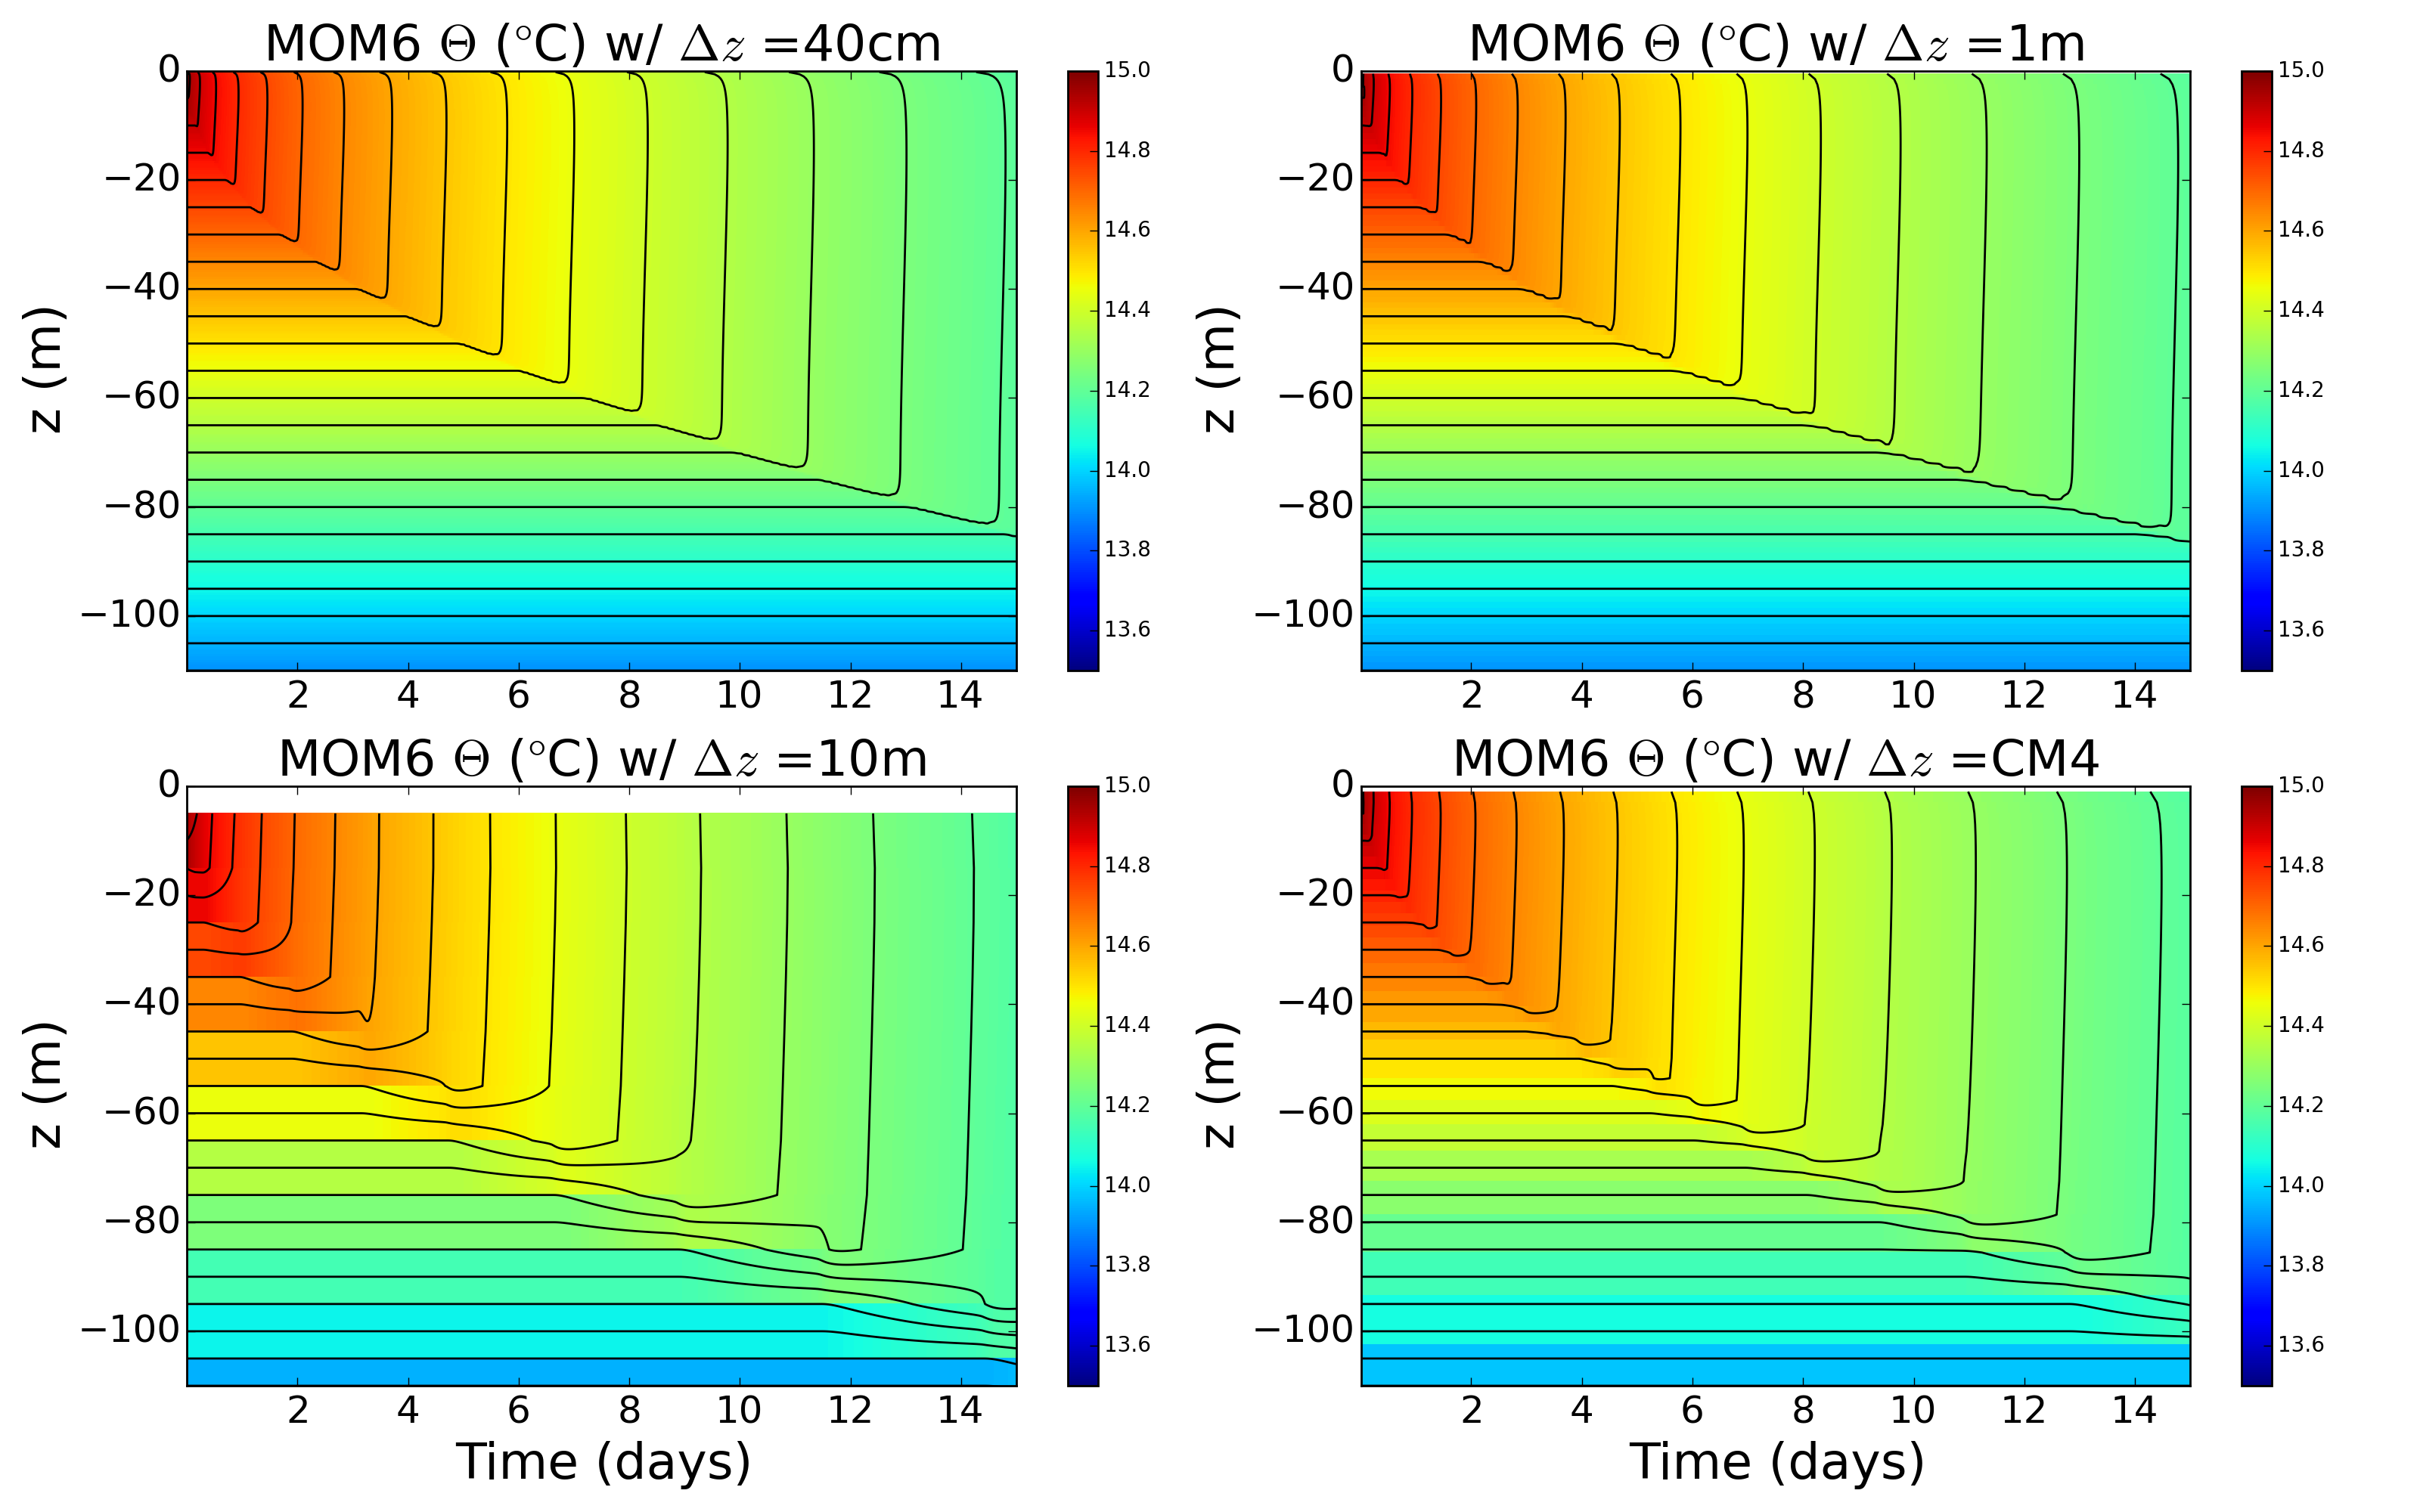
\includegraphics[angle=0,width=14cm]{./figs/MOM6/cooling_KPP_MOM6_temp.png}
\caption[Temperature from MOM6 for cooling test]{\sf Time series for
  temperature from cooling test case (zero wind stress and
  $Q=-100~\mbox{W}~\mbox{m}^{-2}$) as realized in MOM6 using four
  different vertical grid resolutions.}
\label{fig:MOM6_temp-cooling}
\end{center}
%\rule{\textwidth}{0.005in}
\end{figure}
%%%%%%%%%%%%%%%%%%%%%%%%%%%%%%%%%%%%%%%%%%%%%%%%%%%%%%%%%%%%%%%%%%%%%%%%


%%%%%%%%%%%%%%%%%%%% %%%%%%%%%%%%%%%%%%%%%%%%%
\begin{figure}[h!t]
%\rule{\textwidth}{0.005in}
\begin{center}
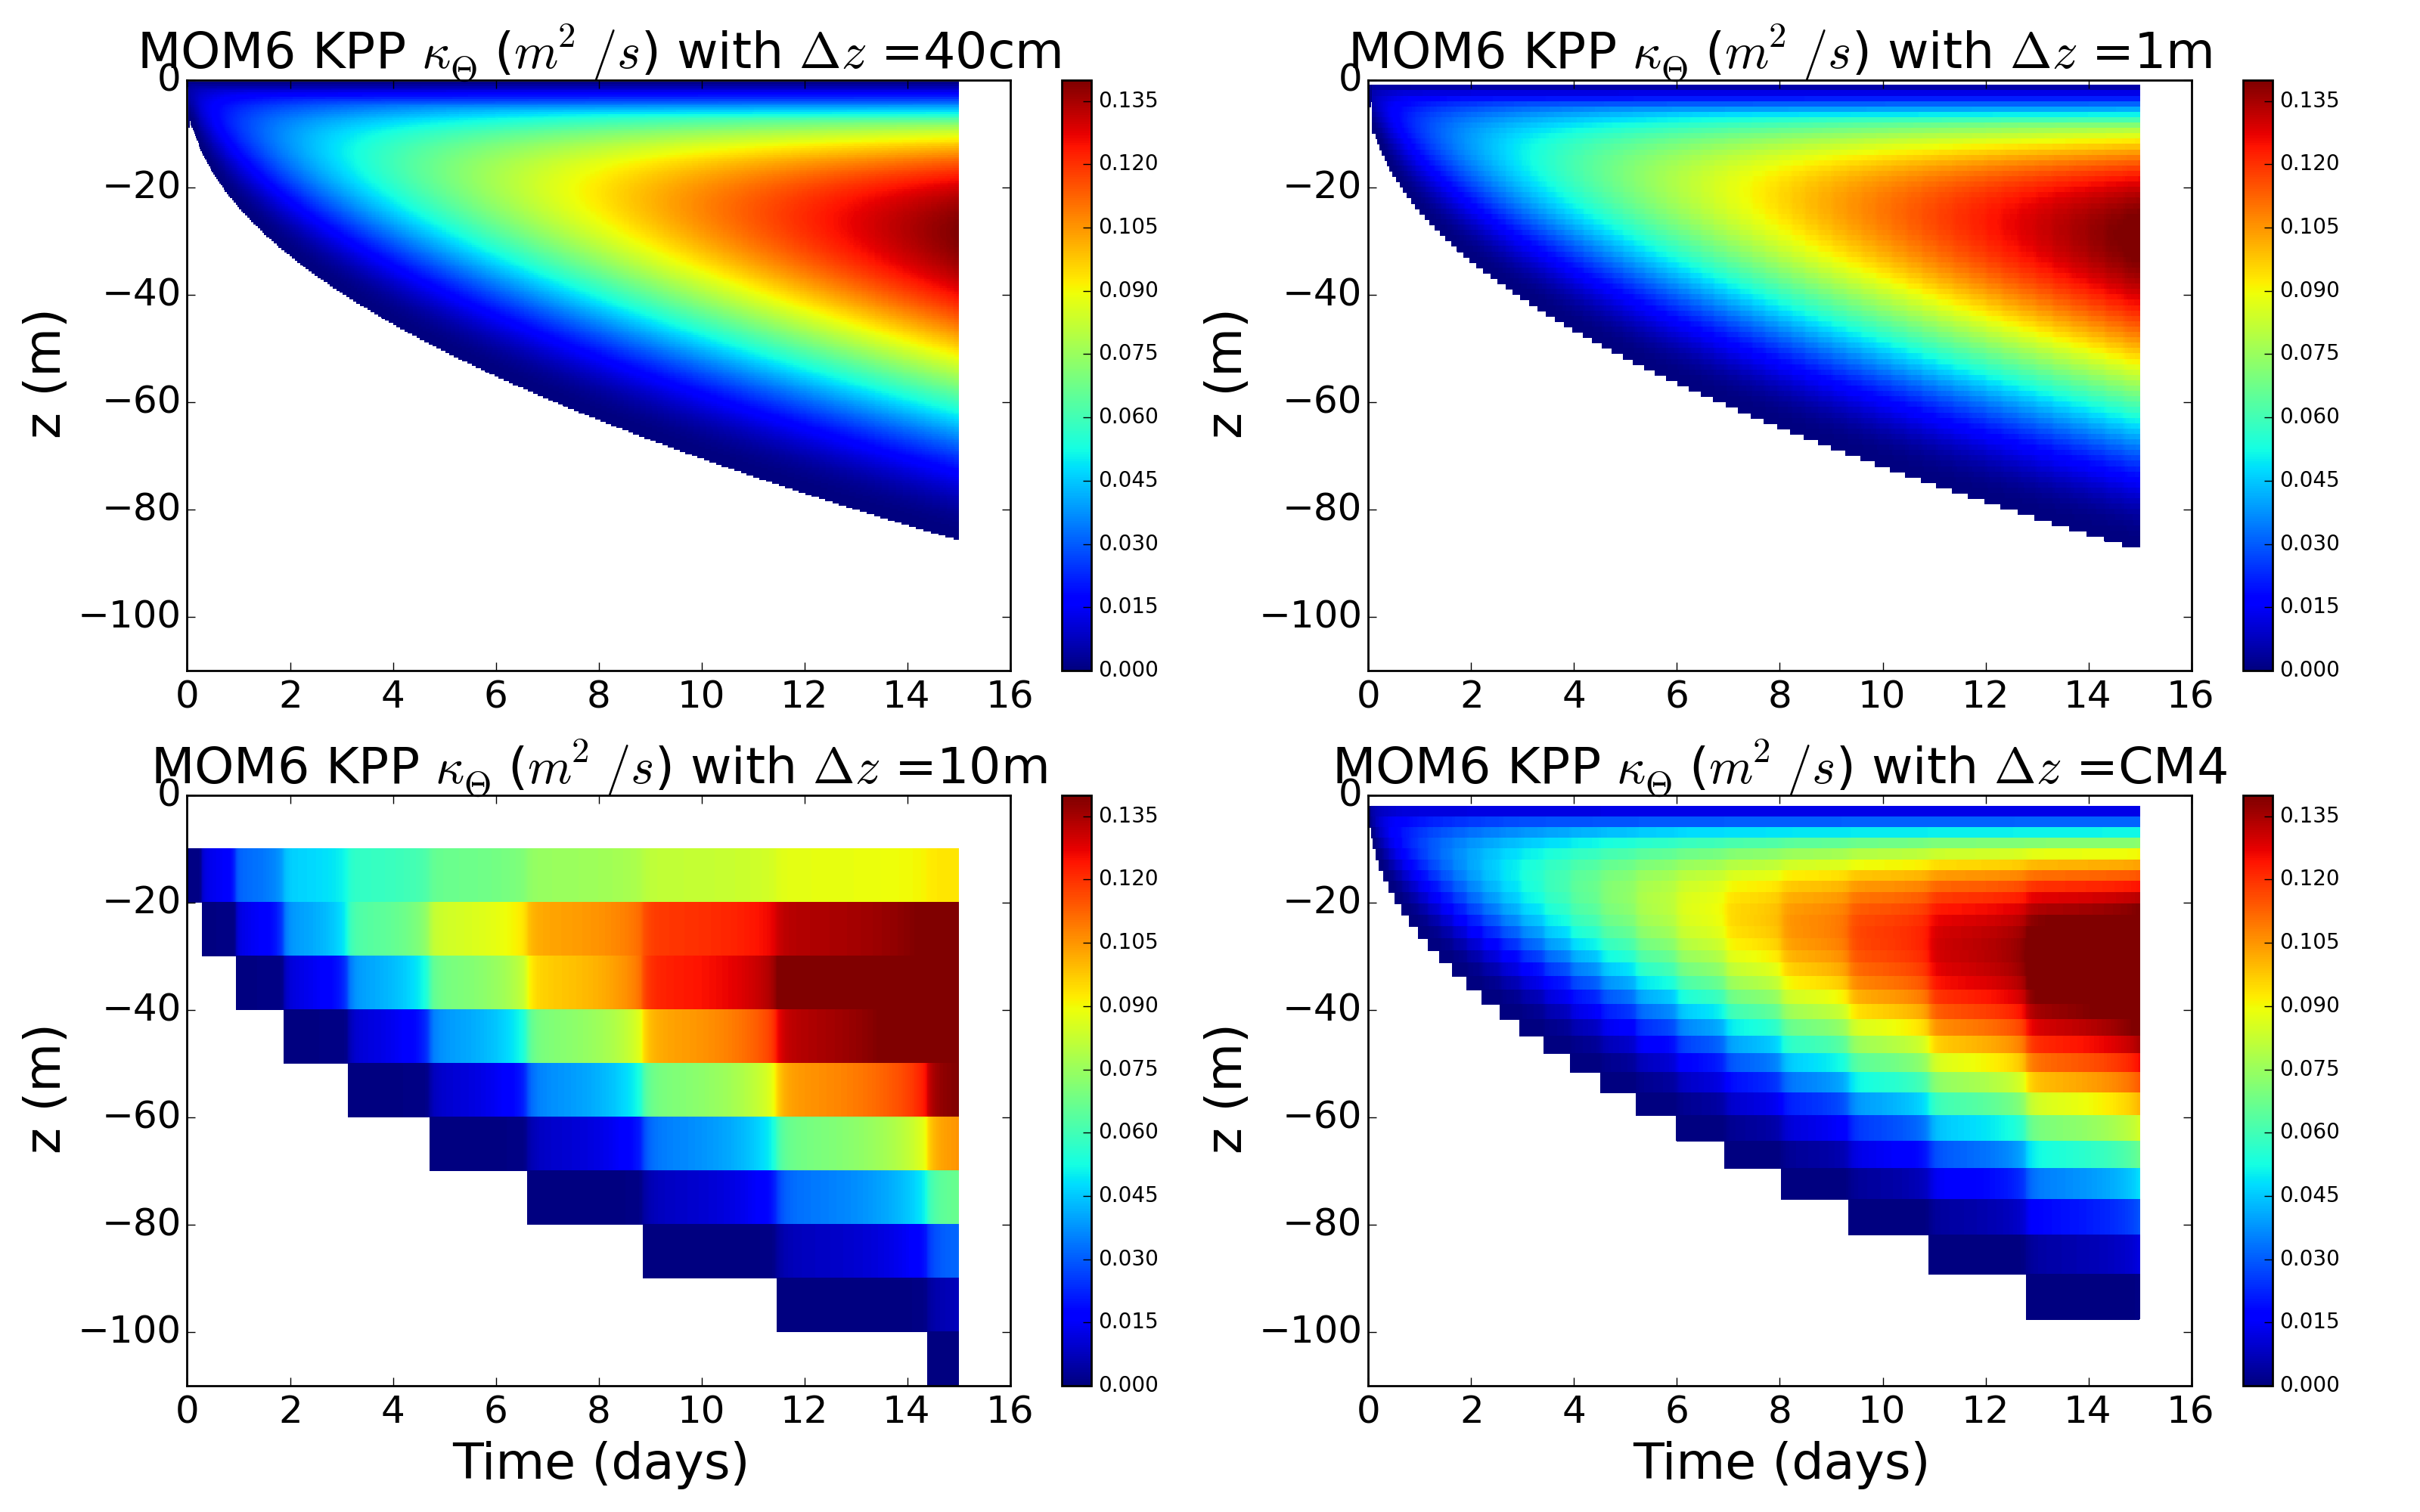
\includegraphics[angle=0,width=14cm]{./figs/MOM6/cooling_KPP_MOM6_KPP_diffusivity.png}
\caption[KPP diffusivity from MOM6 for cooling test]{\sf Time series
  for the KPP vertical diffusivity for cooling test case (zero wind
  stress and $Q=100~\mbox{W}~\mbox{m}^{-2}$) as realized in MOM6 using
  four different vertical grid resolutions.}
\label{fig:MOM6_KPP_diffusivity-cooling}
\end{center}
%\rule{\textwidth}{0.005in}
\end{figure}
%%%%%%%%%%%%%%%%%%%%%%%%%%%%%%%%%%%%%%%%%%%%%%%%%%%%%%%%%%%%%%%%%%%%%%%%


%%%%%%%%%%%%%%%%%%%% %%%%%%%%%%%%%%%%%%%%%%%%%
\begin{figure}[h!t]
%\rule{\textwidth}{0.005in}
\begin{center}
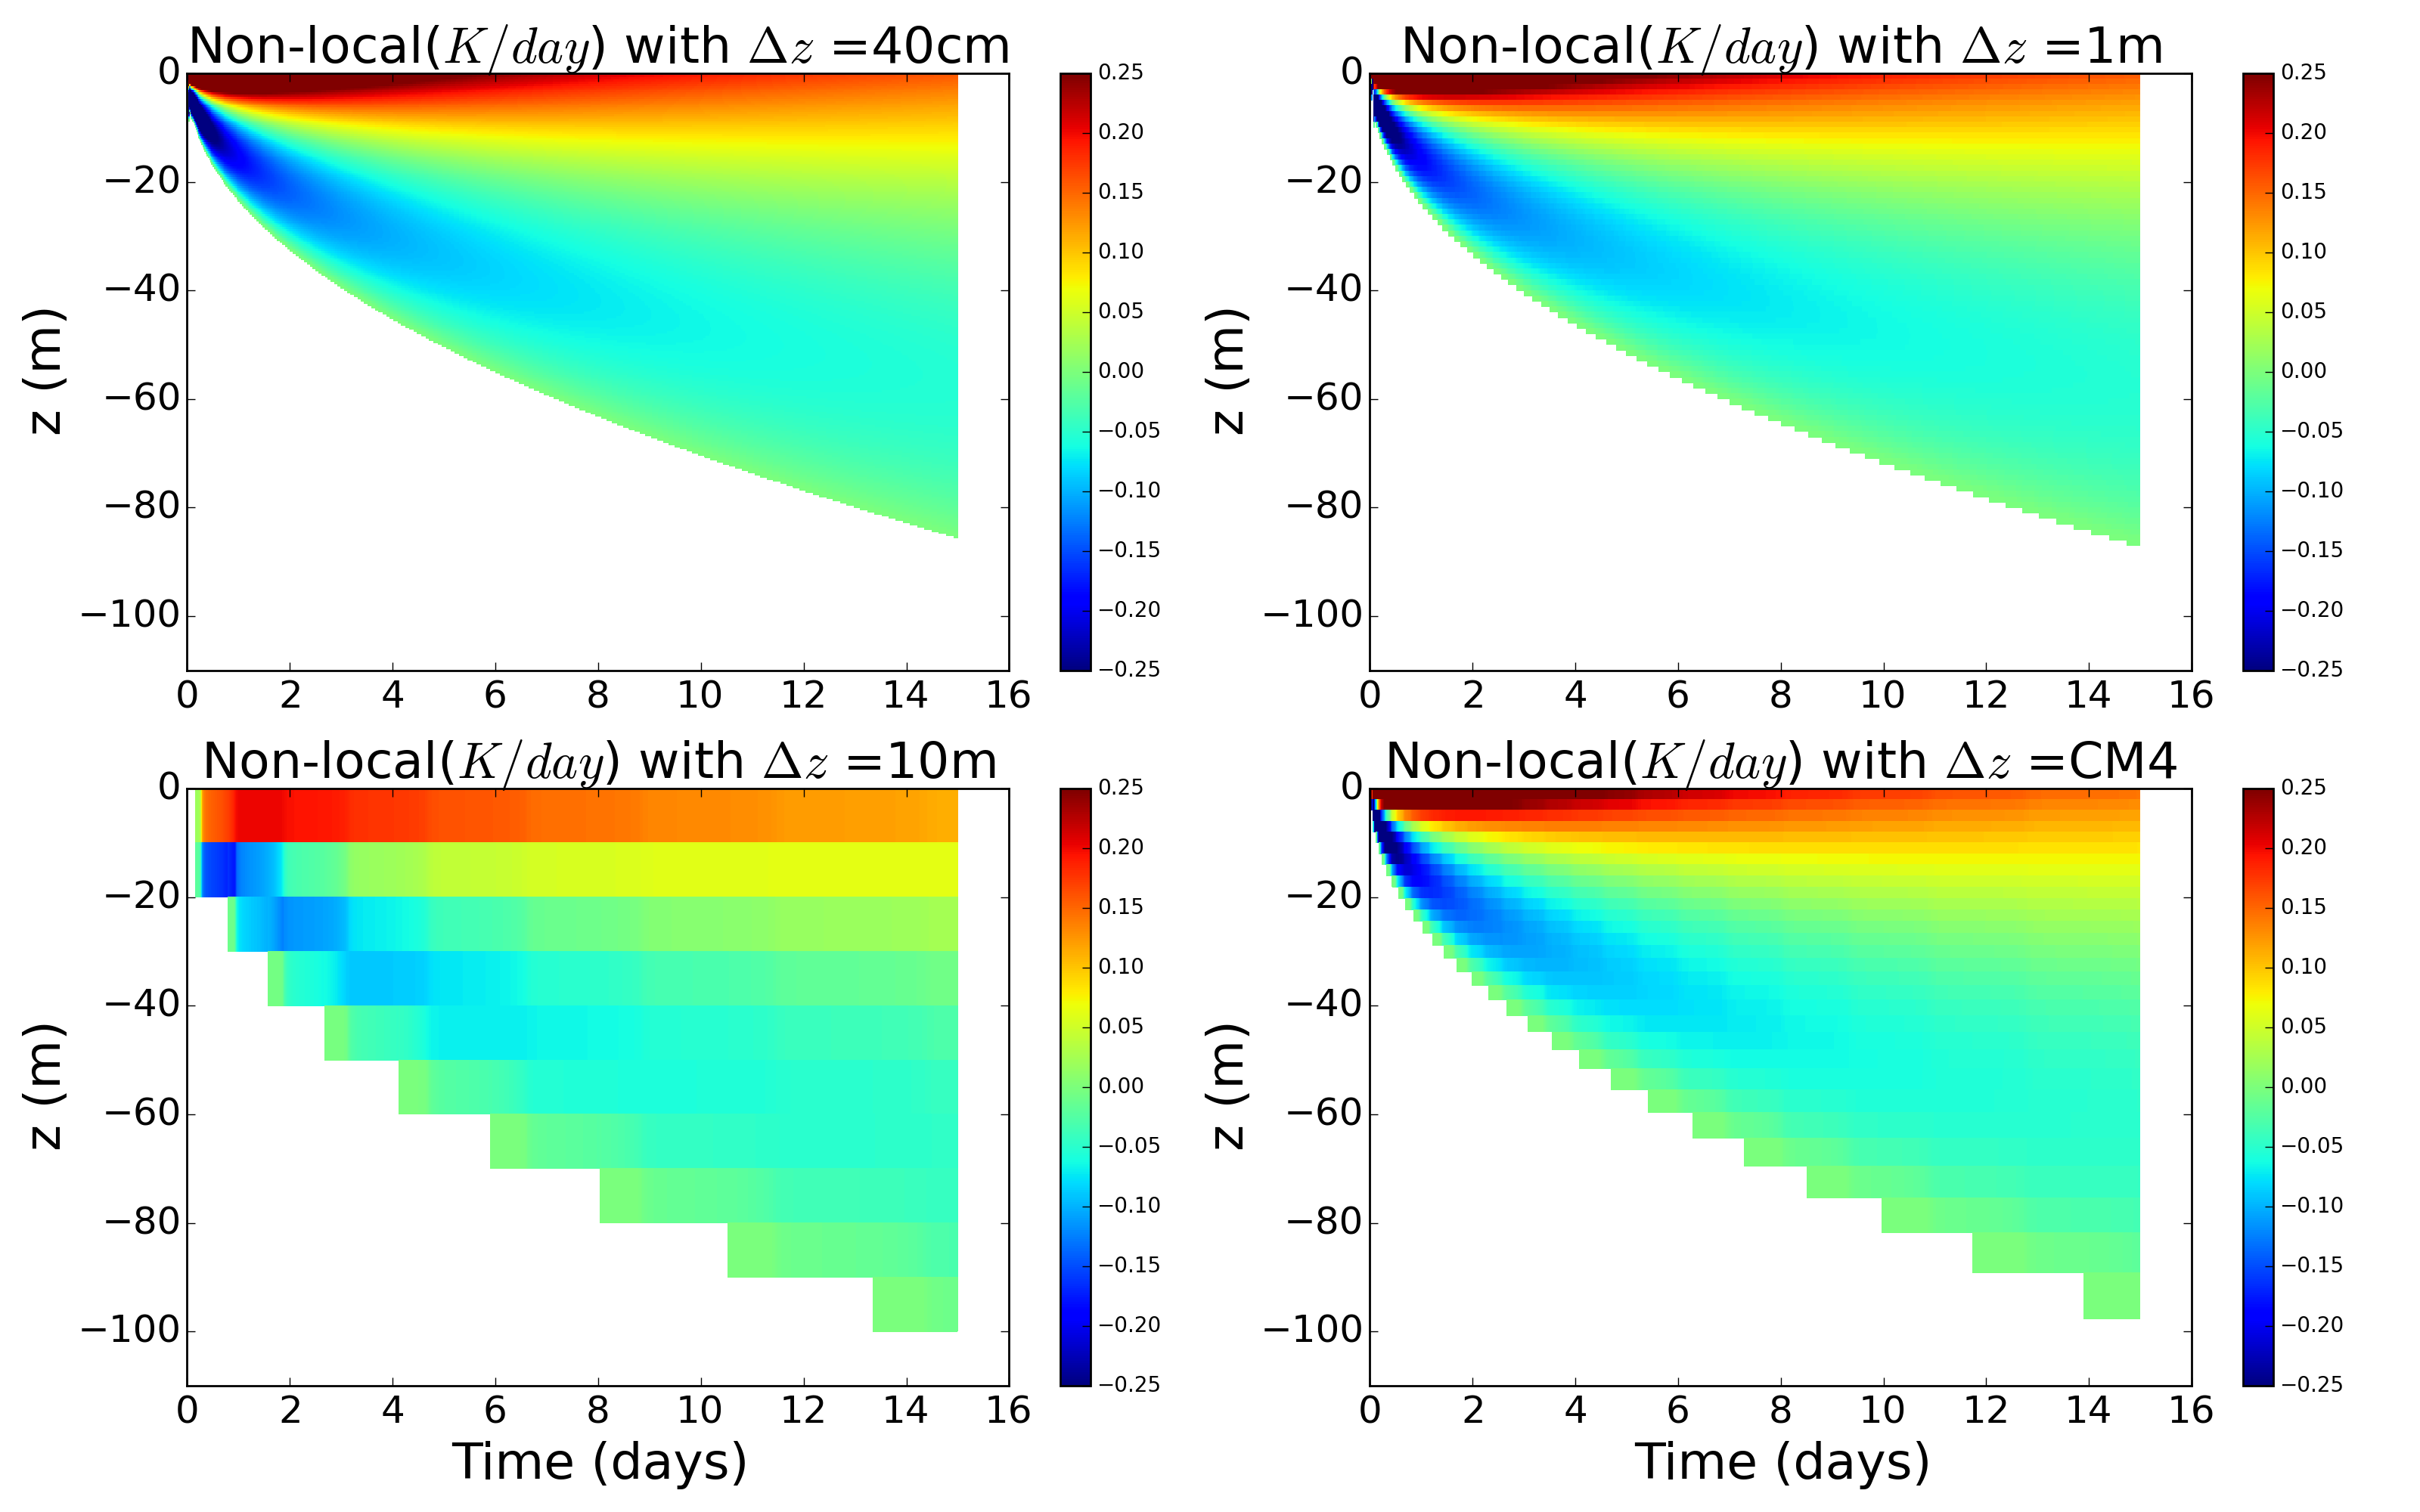
\includegraphics[angle=0,width=14cm]{./figs/MOM6/cooling_KPP_MOM6_nonlocal_temp_tendency.png}
\caption[KPP nonlocal time tendency from MOM6 cooling test]{\sf Time
  series for the time tendency from the KPP non-local transport for
  the cooling test case (zero wind stress and
  $Q=100~\mbox{W}~\mbox{m}^{-2}$) as realized in MOM6 using four
  different vertical grid resolutions.}
\label{fig:MOM6_KPP_nonlocal-cooling}
\end{center}
%\rule{\textwidth}{0.005in}
\end{figure}
%%%%%%%%%%%%%%%%%%%%%%%%%%%%%%%%%%%%%%%%%%%%%%%%%%%%%%%%%%%%%%%%%%%%%%%%






%%%%%%%%%%%%%%%%%%%%%      References     %%%%%%%%%%%%%%%%%%%%%%%%%%%
\newpage 

\bibliographystyle{elsarticle-harv.bst}
\addcontentsline{toc}{chapter}{\scshape Bibliography} 
\markboth{\scshape BIBLIOGRAPHY}{\scshape BIBLIOGRAPHY}
\gdef\rightmark{\scshape BIBLIOGRAPHY}
\bibliography{Griffies_refs}
%%%%%%%%%%%%%%%%%%%%%%%%%%%%%%%%%%%%%%%%%%%%%%%%%%%%%%%%%%%%%%%%%%%%%








\end{document}
